\documentclass[letter,12pt]{article}
%
\newtheorem{lemma}{Lemma}
\newtheorem{proposition}{Proposition}
\newtheorem{theorem}{Theorem}
\newtheorem{definition}{Definition}
\newtheorem{corollary}{Corollary}
\newtheorem{remark}{Remark}

\newcommand{\argmin}{\mathop{^\rm argmin}}
\newcommand{\argmax}{\mathop{\rm argmax}}
\newcommand{\rank}{\mathop{\sf rank}}
\newcommand{\iprod}[2]{\langle #1, #2 \rangle}
\newcommand{\lmin}{\lambda_{\min}}
\newcommand{\norm}[1]{\left\|#1\right\|}
\newcommand{\mge}{\succeq}
\newcommand{\mi}{{-1}}
\newcommand{\R}{\mathbb{R}}\newcommand{\B}{\mathbb{B}}\newcommand{\Id}{\mathbf{I}}
\newcommand{\zerovec}{\mathbf{0}}
\newcommand{\onevec}{\mathbf{1}}
\newcommand{\defeq}{:=}
\newcommand{\secref}[1]{Section~\ref{#1}}
\newcommand{\lemref}[1]{Lemma~\ref{#1}}
\newcommand{\proref}[1]{Proposition~\ref{#1}}
\newcommand{\thmref}[1]{Theorem~\ref{#1}}
\newcommand{\assref}[1]{Assumption~\ref{#1}}
\newcommand{\eqnref}[1]{(\ref{#1})}
\newcommand{\algref}[1]{Algorithm~\ref{#1}}

\newcommand{\Prob}{\mathbb{P}}
\newcommand{\E}{\mathbb{E}}
\newcommand{\V}{\mathbb{V}}
\newcommand{\tr}[1]{\textrm{tr}\left(#1\right)}
%\newcommand{\dt}[1]{\textrm{det}\left(#1\right)}

\newcommand{\Evt}{\mathcal{E}}
\newcommand{\EvtG}{\Evt_G}
\newcommand{\EvtD}{\Evt_\Delta}
\newcommand{\EvtX}{\Evt_X}

\newcommand{\lihong}[1]{[[\textbf{LL:} #1]]}
\renewcommand{\lihong}[1]{}

\newcommand{\RN}[1]{%
  \textup{\uppercase\expandafter{\romannumeral#1}}%
}

\newtheorem{assumption}{Assumption}

\usepackage[table]{xcolor}
\usepackage{relsize}
\usepackage{bm}
\usepackage{mathrsfs}
\usepackage{textcomp} % for inverted comma after Sobol
\newcommand{\angstrom}{\mbox{\normalfont\AA}}

 \def\ol{\overline}
 \def\no{\noindent}
 \def\qd{\dot{Q}}
%%%%%%%FLOW DIAGRAM%%%%%%%%%%
\usepackage[latin1]{inputenc}
\usepackage{tikz}
%\usepackage[table]{xcolor}
\usetikzlibrary{shapes,arrows}
% Define block styles
\tikzstyle{decision} = [diamond, draw, fill=blue!20, 
   text width=5.0em, text badly centered, node distance=3cm, inner sep=0pt]
\tikzstyle{block} = [rectangle, draw, fill=cyan!20, 
   text width=9.0em, text centered, rounded corners]
\tikzstyle{line} = [draw, -latex']
\tikzstyle{cloud} = [draw, ellipse,fill=red!20, node distance=3cm,
   minimum height=2em]
%%%%%%%%%%%%%%%%%%%%%%%%%%
%% Algorithm %%%%%
\usepackage{algorithm,algpseudocode,float}
\usepackage{lipsum}
\makeatletter
\newenvironment{breakablealgorithm}
  {% \begin{breakablealgorithm}
   \begin{center}
     \refstepcounter{algorithm}% New algorithm
     \hrule height.8pt depth0pt \kern2pt% \@fs@pre for \@fs@ruled
     \renewcommand{\caption}[2][\relax]{% Make a new \caption
       {\raggedright\textbf{\ALG@name~\thealgorithm} ##2\par}%
       \ifx\relax##1\relax % #1 is \relax
         \addcontentsline{loa}{algorithm}{\protect\numberline{\thealgorithm}##2}%
       \else % #1 is not \relax
         \addcontentsline{loa}{algorithm}{\protect\numberline{\thealgorithm}##1}%
       \fi
       \kern2pt\hrule\kern2pt
     }
  }{% \end{breakablealgorithm}
     \kern2pt\hrule\relax% \@fs@post for \@fs@ruled
   \end{center}
  }
\makeatother
\algdef{SE}[DOWHILE]{Do}{doWhile}{\algorithmicdo}[1]{\algorithmicwhile\ #1}%
%%%%%%%%%%%%%%%%%

%-------------------------------------------------------------------
\begin{document}

\thispagestyle{empty}
\begin{center}
\textsc{
Uncertainty Quantification in Non-Equilibrium Molecular Dynamics Simulations of
Thermal Transport
}

\bigskip 
\bigskip 

Manav Vohra$^{1}$, Ali Yousefzadi Nobakht$^{2}$, Seungha Shin$^{2}$, Sankaran Mahadevan$^{1}$

\bigskip
\bigskip

\normalsize
$^1$Department of Civil and Environmental Engineering\\
Vanderbilt University\\
Nashville, TN 37235\\

\bigskip

$^2$Department of Mechanical, Aerospace, and Biomedical Engineering\\
The University of Tennessee\\
Knoxville, TN 37996\\

\bigskip

\end{center}

%\vspace{6cm}
%
%\begin{tabbing}
%Corresponding Author: \hspace{5mm} \= Sankaran Mahadevan\\
%       \>  Department of Civil and Environmental Engineering\\
%       \>  Vanderbilt University\\
%       \>  272 Jacobs Hall, VU Mailbox: PMB 351831 \\
%       \>  Nashville, TN 37235 \\
%       \> \\
%Phone: \> (615) 322-3040 \\
%Fax:   \> (615) 343-3773 \\
%Email: \>  sankaran.mahadevan@vanderbilt.edu   \\
%\\
%Submitted to: \> \textit{International Journal of Heat and Mass Transfer} \\
%\>  April 2018\\
%
%\bigskip
%\end{tabbing}
%
%\clearpage



\baselineskip=22pt

%\tableofcontents
%\clearpage

\begin{abstract}
\label{sec:abstract}

%% 1. what is the problem 
Scientific applications that run on leadership computing facilities often face the challenge 
of being unable to fit leading science cases onto accelerator devices due to memory constraints 
(memory-bound applications).
%
% 2. what is your solution 
In this work, the authors studied one such US Department of Energy mission-critical condensed matter 
physics application, Dynamical Cluster Approximation (DCA++), and this paper discusses how device memory-bound challenges were successfully reduced  by proposing an effective 
``all-to-all'' communication method---a ring communication algorithm. 
%
This implementation takes advantage of acceleration on GPUs and remote direct memory access (RDMA) for fast data exchange between GPUs. 
%
\\Additionally, the ring algorithm was optimized with sub-ring communicators
and multi-threaded support to further reduce communication overhead and 
expose more concurrency, respectively.
%
% 3. What's the cherry-picked evaluation result you want to mention
The computation and communication were also analyzed 
by using the Autonomic Performance Environment for Exascale 
(APEX) profiling tool,  and this paper further discusses the 
performance trade-off for the ring algorithm implementation. 
%
The memory analysis on the ring algorithm shows that the allocation size for the authors' most 
memory-intensive data structure per GPU is now reduced to $1/p$ of the original size, where $p$ is the number of GPUs in the ring communicator.
%
The communication analysis suggests that 
the distributed Quantum Monte Carlo execution time grows linearly as sub-ring size increases, and the cost of messages passing through the network interface connector could be a limiting factor.


%
% \todoRed{Ronnie: Next sentence needs rewrite, too much information about Green's function that no one knows in the abstract; recommend generalizing.} \emph {However, DCA++ is currently facing memory-bound challenge as 
% a larger device array $G_t$ is limited by device memory size, where
% $G_t$ is a two-particle Green's function that allows condensed matter
% scientists to explore larger and more complex (higher fidelity)
% physics cases.}

\end{abstract}

\keywords{DCA++, Quantum Monte Carlo, GPU Remote Direct Memory Access, memory-bound issue, exascale machines}

%\clearpage

Reinforcement learning has achieved great success in areas such as Game-playing \citep{silver2018general,vinyals2019grandmaster}, robotics \cite{kober2013reinforcement}, large language models \citep{ouyang2022training}, etc.
However, due to safety concerns or physical limitations, in some real-world reinforcement learning problems, we must consider additional constraints that may influence the optimal policy and the learning process \citep{garcia2015comprehensive}.
% For example, a robotic arm must not take actions that may cause harm to itself or the environments.
A standard framework to handle such cases is the constrained Markov Decision Process (CMDP) \citep{altman1999constrained}.
Within the CMDP framework, the agent has to maximize
the expected cumulative reward while
obeying a finite number of constraints, which are usually in the form of expected cumulative cost criteria.

However, we are sometimes concerned with the problem with a continuum of constraints.
For example,
the constraints we meet might be time-evolving or subject to uncertain parameters, which
cannot be formulated as an ordinary CMDP
(see Examples \ref{Example_Time_Evolving} and  \ref{Example_Uncertain}).
In this paper we would study a generalized CMDP  
to address the above problem.  Because the constraints are not only infinite-number but also lie
in a continuous set,
the generalization is not trivial. Fortunately, we find that we can borrow the idea behind semi-infinite programming (SIP) \citep{remez1934determination, hettich1993semi} to deal with the semi-infinite constraints.
Accordingly, we propose \emph{semi-infinitely constrained Markov decision processes} (SICMDPs)
as a novel complement to the ordinary CMDP framework.
%More specifically,  an SICMDP model %, we consider 
%contains a continuum of constraints whereas an ordinary CMDP contains a finite number of constraints. 

%This generalization is natural but not trivial. However, we can brows the idea  
%The idea is quite natural and can be backtracked
%to the practice of extending linear programming to linear semi-infinite programming (LSIP) %\cite{remez1934determination, GobernaLSIO1998}.
%In addition, 
%As a complementary approach to the ordinary CMDP framework, 
%SICMDP can be used to model these problems  which cannot be described by a finite number of constraints
%that are not covered by .
%For example,
%the restrictions we consider can be time-evolving or subject to uncertain parameters
%, thus
%cannot be described by a finite number of constraints but a continuum of constraints 
%(see Examples \ref{Example_Time_Evolving} and  \ref{Example_Uncertain}).

We also present two reinforcement learning algorithms to solve SICMDPs called SI-CRL and SI-CPO, respectively.
SI-CRL is a model-based reinforcement learning algorithm designed for tabular cases, and SI-CPO is a policy optimization algorithm for non-tabular cases.
% and analyze its performance both theoretically and empirically.
The main challenge is that we need to deal with a continuum of constraints, thus reinforcement learning algorithms for ordinary CMDPs do not work anymore.
In SI-CRL, we tackle this difficulty by first transforming the reinforcement learning problem to an equivalent LSIP problem, which can then be solved using methods in the LSIP literature like the dual exchange methods \citep{Hu1990,reemtsen1998numerical}.
In SI-CPO, we resort to the idea of cooperative stochastic approximation developed in \cite{lan2020algorithms, wei2020comirror}.
As far as we know, we are the first to introduce tools from semi-infinitely programming (SIP) into the reinforcement learning community for solving constrained reinforcement learning problems.

% To the best of our knowledge, we are the first to apply tools from semi-infinitely programming (SIP) to solve reinforcement learning problems.
Furthermore, we give theoretical analysis for both SI-CRL and SI-CPO.
We decompose the error of SI-CRL into two parts: the statistical error from approximating the true SICMDP with an offline dataset and the optimization error due to the fact that the solution of the LSIP problem obtained by the dual exchange method is inexact.
On the optimization side, we show that the iteration complexity of SI-CRL is $O\left(\left\{\mathrm{diam}(Y)L\sqrt{|\gS|^2|\gA|m}/\left[(1-\gamma)\epsilon\right]\right\}^m\right)$.
On the statistical side, we show that the sample complexity of SI-CRL is $\widetilde O\left(\frac{|S|^2|A|^2}{\epsilon^2(1-\gamma)^3}\right)$ if the offline dataset is generated by a generative model, and $\widetilde O\left(\frac{|S||A|}{\nu_{\min} \epsilon^2(1-\gamma)^3}\right)$ if the dataset is generated by a probability measure $\nu$ as considered in \cite{chen2019information}.
Here $\widetilde O$ means that all logarithm terms are discarded.
For SI-CPO, things become a little more complicated because other than the statistical error and the optimization error, we also need to consider the function approximation error, which comes from imperfect policy parametrizations.
It is shown if the function approximation error can be controlled to $O(\epsilon)$ order, the iteration complexity of SI-CPO is $\widetilde{O}\left(\frac{1}{\epsilon^2(1-\gamma)^6}\right)$ and the sample complexity of SI-CPO is $\widetilde{O}(\frac{1}{\epsilon^4(1-\gamma)^{10}})$.
Here our iteration complexity bound is equivalent to a typical $\widetilde O(1/\sqrt{T})$ global convergence rate.

We perform a set of numerical experiments to illustrate the SICMDP model and validate our proposed algorithms.
Specifically, we examine two numerical examples, namely the discharge of sewage and ship route planning.
Through the discharge of sewage example, we show the advantage of the SICMDP framework over the CMDP baseline obtained by naive discretization in modeling realistic sequential decision-making problems.
Moreover, we demonstrate the effectiveness of the SI-CRL and SI-CPO algorithms in such tabular environments. 
In the ship route planning example, we illustrate the benefits of the SICMDP framework and the ability of the SI-CPO algorithm to address complex continuous control tasks involving continuous state spaces with modern deep reinforcement learning techniques.

% In summary, our contributions are listed as follows.
% First, we present the SICMDP model, which can be viewed as a generalization of the ordinary CMDP model.
% Second, we propose an algorithm to perform reinforcement learning for SICMDPs, which is called SI-CRL, and we believe that we are the first to apply tools from SIP
% to solve reinforcement learning problems.
% Third, we give a theoretical analysis of SI-CRL and identify both its sample complexity and iteration complexity.
% In addition, we perform numerical experiments to illustrate the SICMDP model and validate the SI-CRL algorithm.
% \{This paragraph can be removed!!! \}





\bigskip
\bigskip
%
%
\vspace{-0.1in}
\section{Neural Program Synthesis from Input-Output Examples}
\vspace{-0.1in}
In programming by example tasks, the program specification is a set of input-output examples~\cite{devlin2017robustfill,bunel2018leveraging}. Specifically, we provide the synthesizer with a set of $K$ input-output pairs $\{(I^{(k)}, O^{(k)})\}_{k=1}^K$ ($\{IO\}^K$ in short). These input-output pairs are annotated with a ground truth program $P^\star$, so that $P^\star(I^{(k)})=O^{(k)}$ for any $k \in \{1, 2, ..., K\}$. To measure the program correctness, we include another set of held-out test cases $\{IO\}_{test}^{K_{test}}$ that differs from $\{IO\}^K$. The goal of the program synthesizer is to predict a program $P$ from $\{IO\}^K$, so that $P(I)=P^\star(I)=O$ for any $(I, O) \in \{IO\}^K + \{IO\}_{test}^{K_{test}}$.

%\label{sec:c-data}
\textbf{C Program Synthesis}. In this work, we make the first attempt of synthesizing C code in a restricted domain from input-output examples only, and we focus on programs for list processing. List processing tasks have been studied in some prior works on input-output program synthesis, but they synthesize programs in restricted domain-specific languages instead of full-fledged popular programming languages~\cite{balog2016deepcoder,odena2020learning,odena2020bustle}. 

Our C code synthesis problem brings new challenges for programming by example. Compared to domain-specific languages, the syntax and semantics of C are much more complicated, which significantly enlarges the program search space. Meanwhile, learning good representations for partially decoded programs also becomes more difficult. In particular, prior neural program synthesizers that utilize per-line interpreters for the programming language to guide the synthesis and representation learning~\cite{chen2018execution,shin2018improving,nye2020representing,Ellis2019WriteEAExtendExecution,odena2020bustle} are not directly applicable to C. Although it is possible to dump some intermediate variable states during C code execution~\cite{campbell2012executable}, since partial C programs are not executable, we are able to obtain all the execution states only until a full C code is generated, which is too late to include them in the program decoding process. In particular, the intermediate execution state is not available when the partial program is syntactically invalid, and this happens more frequently for C due to its syntax design.
\begin{figure}
    \centering
    \includegraphics[width=\textwidth]{fig/c-program-synthesis-crop.pdf}
\caption{\small Illustration of the C program synthesis pipeline. For dataset construction, we develop a random program generator to sample random C programs, then execute the program over randomly generated inputs and obtain the outputs. The input-output pairs are fed into the neural program synthesizer to predict the programs. Note that the synthesized program can be more concise than the original random program.}
\label{fig:ex-c}
\end{figure}


\bigskip
\bigskip
%%
%%
\documentclass[12pt]{article}
\usepackage{amsmath}
\usepackage{enumerate}
\usepackage{xr}
%\externaldocument{epinet}
\newcommand{\fullspace}{\mathfrak{N}}

\pdfminorversion=4
\usepackage{url} 

\newcommand{\czero}{[C.1]}
\newcommand{\cone}{[C.2]}
\newcommand{\ctwo}{[C.3]}
\newcommand{\cthree}{\mbox{[C.4]}}
\newcommand{\cfour}{[C.5]}
\newcommand{\cfive}{[C.6]}

\newcommand{\ghoster}[0]{}

% OLD PREAMBLE:

% \usepackage{jsen}
% \usepackage{cite}
% \usepackage{amsmath,amssymb,amsfonts, bbm, mathtools}
% \usepackage{algorithm,algorithmic}
% \usepackage{graphicx}
% \usepackage{textcomp}
% \usepackage{wrapfig}
% \usepackage{xfrac}
% \usepackage{stackengine}
% \usepackage{subfigure}
% \def\delequal{\mathrel{\ensurestackMath{\stackon[1pt]{=}{\scriptstyle\Delta}}}}



% \usepackage{color, soul}
% \newcommand{\hlt}[1]{\hl{#1}}
% \newcommand{\red}[1]{\textcolor{red}{#1}}

% \def\BibTeX{{\rm B\kern-.05em{\sc i\kern-.025em b}\kern-.08em
%     T\kern-.1667em\lower.7ex\hbox{E}\kern-.125emX}}
% \markboth{\journalname, VOL. XX, NO. XX, XXXX 2017}
% {Author \MakeLowercase{\textit{et al.}}: Preparation of Papers for IEEE TRANSACTIONS and JOURNALS (February 2017)}
% \definecolor{abstractbg}{rgb}{0.89804,0.94510,0.83137}
% \setlength{\fboxrule}{0pt}
% \setlength{\fboxsep}{0pt}

% NEW PREAMBLE:


\usepackage{amsmath,amsfonts,amssymb,bbm, amsthm, xfrac}
\usepackage{algorithmic}
\usepackage{algorithm}
\usepackage{array, multirow}
% \usepackage[caption=false,font=normalsize,labelfont=sf,textfont=sf]{subfig}
\usepackage{caption, subcaption}
\usepackage{textcomp}
\usepackage{stfloats}
\usepackage{url}
\usepackage{verbatim}
\usepackage{graphicx}
\usepackage{cite}
\usepackage{caption}
\usepackage{subcaption}
\hyphenation{}

\theoremstyle{plain}
\newtheorem{theorem}{Theorem}

\usepackage{color, soul}
\newcommand{\hlt}[1]{\hl{#1}}
\newcommand{\red}[1]{\textcolor{red}{#1}}


\RequirePackage[letterpaper, portrait, margin=1in]{geometry}

\usepackage[]{natbib}
\bibpunct{(}{)}{,}{a}{}{,}

\renewcommand{\s}{\vspace{0.1cm}}

\setlength{\bibsep}{0pt plus 0.3ex}
\newcommand{\size}{L}
\newcommand{\norm}[1]{\lVert#1\rVert}

\def\baselinestretch{1.05}
\newcommand{\mQ}{\mathbb{Q}(\bbeta^\star, \bSigma)}
\newcommand{\tr}{\mathop{tr}}
\newcommand{\supp}{\mathbb{S}}
\newcommand{\wm}{\widehat{\rho}}
\newcommand{\btas}{\bta^\star}
\newcommand{\bepsilon}{\bm{\delta}}
\renewcommand{\interior}{\textnormal{int}}
\newcommand{\BBB}{\mathbb{B}}

\newcommand{\compl}{\mbox{comp}}
\renewcommand{\balpha}{a}
\usepackage{amsfonts,amsmath,amssymb,latexsym,bm,bbm}
\newcommand{\mbG}{\mathscr{G}}
\RequirePackage{amsthm,amsmath}
\usepackage{times}
\usepackage{natbib}
\hyphenation{neigh-bor-hood}
\newcommand{\deltaepsilon}{\delta(\epsilon)}
\renewcommand{\bta}{\bm{\eta}}
\renewcommand{\bta}{\bm{\eta}}
\usepackage{multirow}
\newcommand{\GG}{\mathscr{G}(\omega)}
\newcommand{\HH}{\mathscr{G}(\omega_1)}
\usepackage{mathtools}
\newcommand{\comp}{\mbox{comp}\,}
\renewcommand{\one}{\mathbbm{1}}
\renewcommand{\mM}{\mathbb{M}}
\newcommand{\mMs}{\mM(\omega)}
\newcommand{\etaspace}{\bm{\Xi}}
\renewcommand{\mT}{\mathbb{T}}
\usepackage[mathscr]{eucal}
\renewcommand{\bmu}{\bm{\mu}}
\renewcommand{\bA}{\bm{A}}
\renewcommand{\bt}{\bm{t}}
\renewcommand{\bB}{\bm{B}}
\renewcommand{\bC}{\bm{C}}
\renewcommand{\norm}[1]{\lVert#1\rVert}
\renewcommand{\mbR}{\mathbb{R}}
\renewcommand{\lip}{{\tiny\mbox{Lip}}}
\renewcommand{\lte}{&\leq&}
\renewcommand{\gte}{&\geq&}
\renewcommand{\mD}{\mathbb{D}}
\renewcommand{\btheta}{\bm{\theta}}
\renewcommand{\bTheta}{\bm{\Theta}}
\newcommand{\bThetas}{\bm{\Theta}^\star}
\renewcommand{\tends}{\to}
\renewcommand{\tend}{\rightarrow}
\newcommand{\rint}{\mathop{\mbox{rint}}}
\renewcommand{\su}{\sup\limits}
\renewcommand{\mS}{\mathbb{S}}
\renewcommand{\mbX}{\mathbb{X}}
\renewcommand{\mbY}{\mathbb{Y}}
\renewcommand{\uu}{x_i}
\renewcommand{\vv}{x_i^\star}
\renewcommand{\logit}{\mbox{logit}}
\renewcommand{\tv}{{\tiny\mbox{TV}}}
\renewcommand{\mbV}{\mathbb{V}}
\renewcommand{\mB}{\mathscr{B}}
\renewcommand{\BB}{\mathscr{B}}
\renewcommand{\CC}{\mathscr{C}}
\usepackage{bbm,amsfonts,graphicx}

\newcommand{\xk}{\bm{x}_k}
\newcommand{\yk}{\bm{y}_k}
\newcommand{\Xk}{\bm{X}_k}
\newcommand{\Yk}{\bm{Y}_k}
\newcommand{\mXk}{\mX_k}
\newcommand{\mYk}{\mY_k}
\newcommand{\mSS}{\mathbb{S}}
\newcommand{\ppp}{m}
\newcommand{\qqq}{q}
\newcommand{\diminf}{\ppp}
\usepackage{multicol}
\renewcommand{\vec}{\mathop{\mbox{vec}}}
\newcommand{\conv}{\mbox{conv}}
\renewcommand{\bx}{\bm{x}}
\renewcommand{\=}{&=&}
\renewcommand{\hide}[1]{}
\newcommand{\ghost}[1]{}
\renewcommand{\zs}{\bm{z}^\star}
\newcommand{\Thetad}{\Theta_0}
\newcommand{\bthetas}{\btheta^\star}
\newcommand{\thetas}{\theta^\star}
\newcommand{\thetad}{\thetas}
\newcommand{\etas}{\eta^\star}
\newcommand{\bthetad}{{\btheta}_0}
\newcommand{\bThetad}{{\bTheta}_0}
\newcommand{\thetah}{\widehat{\theta}}
\newcommand{\bthetah}{\widehat{\btheta}}
\newcommand{\bthetahh}{\widehat{\bthetah}}
\renewcommand{\mX}{\mathbb{X}}
\renewcommand{\mbT}{\mathbb{T}}
\renewcommand{\mC}{\mathbb{C}}
\renewcommand{\mY}{\mathbb{Y}}
\renewcommand{\mI}{\mathbb{I}}
\renewcommand{\mZ}{\mathbb{Z}}
\renewcommand{\be}{\begin{equation}\begin{array}{lllllllllllllllll}}
\renewcommand{\beno}{\begin{equation}\begin{array}{lllllllllllll}\nonumber}
\renewcommand{\ee}{\end{array}\end{equation}}
\renewcommand{\dis}{\displaystyle}
\renewcommand{\dsum}{\displaystyle\sum\limits}
\renewcommand{\dint}{\displaystyle\int\limits}
\renewcommand{\dprod}{\displaystyle\prod\limits}
\renewcommand{\dd}{\mathop{\mbox{d}}\nolimits}
\renewcommand{\mR}{\mathbb{R}}
\renewcommand{\mbE}{\mathbb{E}}
\renewcommand{\mbP}{\mathbb{P}}
\renewcommand{\mA}{\mathscr{A}}
\newcommand{\mAs}{\mA}
\newcommand{\mF}{\mathscr{F}}
\renewcommand{\mV}{\mathscr{V}}
\newcommand{\mJ}{\nabla_{\btheta}\, \bta(\btheta)}
\renewcommand{\mE}{\mathscr{E}(\delta(\epsilon))}
\renewcommand{\mbG}{\mathscr{G}(\omega)}
\setlength{\topmargin}{-.25in}
\setlength{\topskip}{0in}
\setlength{\oddsidemargin}{0in}
\setlength{\evensidemargin}{0in}
\setlength{\headheight}{0in}
\setlength{\headsep}{0in}
\setlength{\textheight}{9.5in}
\setlength{\textwidth}{6.75in}
\usepackage{hyperref}
\usepackage{xr}
\externaldocument{ergm_algorithm3}

\newcommand{\uuu}{|\ell(\bthetas, \bzs; \bmu^\star)|}
\newcommand{\bzs}{\bz^\star}
\renewcommand{\bbq}{\vspace{.05cm}\begin{quote}\bf``}
\renewcommand{\ebq}{\hspace{-.15cm}"\end{quote}}
\usepackage{etoolbox}
\newcommand{\bauthq}{\vspace{.05cm}\begin{quote}\em}
\newcommand{\eauthq}{\hspace{-.25cm}\end{quote}}
\newcommand{\revisedtitle}{Large-scale estimation of random graph models with local dependence}
\renewcommand{\=}{&=&}

\begin{document}

\thispagestyle{empty}

\begin{center}
{\Large
Manuscript GNST-2020-06-29: Point-by-Point Response
}\s\s
\\
\large
A Semiparametric Bayesian Approach to Epidemics, with Application to the Spread of the Coronavirus MERS in South Korea in 2015
\end{center}

We are indebted to the constructive comments and suggestions of the referees.
We have revised the paper in accordance and respond to the comments and suggestions of the referees point by point.
All major changes in the revised paper are quoted below in full.
In the revised paper,
all major changes are colored red.
We start with a list of the main changes of the revised paper.

\section*{Main changes}

In response to the suggestions of Referee 2,
we have restructured the paper and revised the titles of the sections as follows:
\bi
\item[] Section 1 Motivation
\bi
\item[] Section 1.1 Advantages of network-based approaches to epidemics
\item[] Section 1.2 Shortcomings of existing network-based approaches
\item[] Section 1.3 Proposed network-based approach 
\item[] Section 1.4 Goal: superpopulation inference for finite populations
\item[] Section 1.5 Structure of the paper
\ei
\item[] Section 2 A network-based stochastic model of epidemics
\bi
\item[] Section 2.1 Data-generating process
\item[] Section 2.2 Parametric population models
\ei
\item[] Section 3 Shortcomings of parametric population models
\item[] Section 4 Semiparametric population model
\bi
\item[] Section 4.1 Detecting potential superspreaders
\item[] Section 4.2 Short- and long-tailed degree distributions
\ei
\item[] Section 5 Incomplete data
\bi
\item[] Section 5.1 Possible reasons for incomplete data
\item[] Section 5.2 Importance of collecting network data
\ei
\item[] Section 6 Bayesian inference
\bi
\item[] Section 6.1 Complete- and incomplete-data generating process
\item[] Section 6.2 Bayesian inference based on incomplete data
\item[] Section 6.3 Truncated Dirichlet process priors
\item[] Section 6.4 Bayesian Markov chain Monte Carlo algorithm
\item[] Section 6.5 Addressing the label-switching problem
\ei
\item[] Section 7 Simulation results
\bi
\item[] Section 7.1 Simulation results quantifying the error of estimation
\item[] Section 7.2 Simulation results quantifying the effect of network sampling
\ei
\item[] Section 8 Partially observed MERS epidemic in South Korea
\bi
\item[] Section 8.1 Data
\item[] Section 8.2 Model
\item[] Section 8.3 Computing
\item[] Section 8.4 Results
\ei
\item[] Section 9 Open questions and directions for future research
\bi
\item[] Section 9.1 What is the population of interest?
\item[] Section 9.2 Incomplete data
\item[] Section 9.3 Computational challenges arising from incomplete data
\item[] Section 9.4 Non-ignorable incomplete-data generating processes
\item[] Section 9.5 Population models capturing additional network features
\item[] Section 9.6 Time-evolving population contact networks
\ei
\ei

We hope that these changes in the structure of the paper make the different contributions of the paper more visible.
In addition,
we have made the following changes:
\bi
\item We have inserted a table of contents between the abstract and the introduction of the paper.
\item In response to the comments and suggestions of Referees 1 and 2,
we have changed the application to the MERS data set by 
\bi
\item[---] increasing the number of subpopulations from $K=2$ to $K=3$;
\item[---] adding posterior predictions of the degree distribution;
\item[---] assessing the sensitivity of posterior predictions of the epidemic to the choice of prior;
\item[---] adding more detailed descriptions of data, model, and results.
\ei
\item We have tightened the writing of the paper and have revised the supplement of the paper in accordance with the paper.
\ei

\vspace{-.3cm}

\section*{Referee 1}

\bbq
Summary. 

This paper proposes a flexible semiparametric Bayesian approach to deal with incomplete observations of stochastic processes governing the spread of infectious diseases. The developed methodology is applied to study spread of the coronavirus MERS in South Korea in 2015. After reading the paper, I have the following major concerns.

1. The number of population members N is assumed to be finite in Section 2.1. Would the proposed semiparametric Bayesian method be applicable to the case when N tends to infinity.
\ebq

Thank you for your question,
which touches important statistical issues.
We have addressed these issues in the revised submission by adding the following subsection to the introduction of the paper:
\vspace{-.4cm}
\bauthq
\subsubsection*{1.4 Goal: superpopulation inference for finite populations}
The proposed semiparametric modeling framework,
based on infinite mixture distributions and Dirichlet process priors \citep{Fe73,Teh2007},
extends to infinite populations.
That said,
we assume that the number of population members $N$ is finite and embrace a superpopulation approach to statistical inference along the lines of \citet{hartley1975super} and \citet*{ScKrBu17},
motivated by applications.

The assumption of finite $N$ is motivated by the fact that in epidemiological applications the number of population members $N$ cannot be infinite.
For example,
when the population of interest consists of all animals or all humans on earth,
the size of the population is bounded above by real-world constraints such as geography and the scarcity of natural resources:
Planet earth cannot host infinite populations of animals or humans.

Since the population of interest is finite,
the natural objective of statistical inference is to learn the stochastic process that generated the population contact network and allows infectious diseases to spread through the population of interest,
with a view to understanding and predicting epidemics in the population of interest and similar populations.
In other words,
it is natural to embrace a superpopulation approach to statistical inference,
as discussed by \citet{hartley1975super} and \citet{ScKrBu17}.
The properties of statistical procedures for superpopulation inference can be understood by developing a non-asymptotic statistical theory that relies on concentration inequalities and other non-asymptotic tools that have been embraced in high-dimensional statistics \citep[see, e.g.,][]{Wa19}.
We are not aware of non-asymptotic statistical theory for stochastic models of epidemics,
although there are asymptotic results in probability theory \citep*[e.g.,][]{Re95,BrLiTu11,BaRe13,PaPa20,Ba21} and statistical theory \citep[e.g.,][]{Br98,Br01a} based on $N \to \infty$ asymptotics.
Developing non-asymptotic statistical theory for stochastic models of epidemics constitutes an interesting direction for future research,
but is beyond the scope of our paper.
\eauthq

\bbq
2. The degree parameters $\theta_1$, $\theta_2$, $\dots$, $\theta_N$ are assumed to be generated by a Diricklet process prior. Are the proposed Bayesian estimates sensitive to the prior choice?
\ebq

Thank you for bringing up an important point.
The posterior is sensitive to the choice of prior,
but the Dirichlet process prior is not the primary issue:
While a Dirichlet process prior with concentration parameter $\alpha$ and base distribution $N(\mu,\, \sigma^2)$ does depend on the hyperparameters $\alpha$, $\mu$, and $\sigma^2$,
the hyperparameters $\alpha$, $\mu$, and $\sigma^2$ are not specified by investigators but are random and have hyperpriors.
In Section 6.3 of the revised submission,
we point out:
\bauthq
Since the concentration parameter $\alpha$ and the parameters $\mu$ and $\sigma^2$ of the base distribution $N(\mu,\, \sigma^2)$ are unknown,
it is natural to express the uncertainty about $\alpha$, $\mu$, and $\sigma^2$ by assuming that $\alpha$, $\mu$, and $\sigma^2$ have hyperpriors.
%In other words,
%the knowledge about the hyperparameters $\alpha$, $\mu$, and $\sigma^2$ is updated in the light of the observed data:
%The Bayesian Markov chain Monte Carlo algorithm described in Section 6.4 can be used to approximate the marginal posteriors of the hyperparameters $\alpha$, $\mu$, and $\sigma^2$ given the observed data,
%although the hyperparameters are not the primary target of statistical inference.
We assume that the hyperpriors of the hyperparameters $\alpha$, $\mu$, and $1 / \sigma^{2}$ are Gamma, Gaussian, and Gamma distributions,
respectively,
which are conjugate priors and facilitate Markov chain Monte Carlo sampling from the posterior distribution.

\eauthq
The primary issue is that the posterior is sensitive to the prior probabilities of who infected whom,
because the MERS data set does not contain direct observations of transmissions or contacts,
so the information on transmissions and contacts is limited to two sources of indirect observations:
\bi
\item The assessments of doctors of who infected whom,
which we use to specify the prior probabilities of who infected whom.
\item The observed infectious and removal times,
which reveal when infected population members were infectious and therefore help narrow down the possible sources of infections.
\ei
While the observed infectious and removal times help narrow down the possible sources of infections,
there may be many possible sources of infections left.
As a consequence,
it is not surprising that the posterior is sensitive to the choice of prior probabilities of who infected whom.

We demonstrate in Section 8.4 of the revised submission that posterior predictions of the epidemic are sensitive to the choice of prior probabilities of who infected whom:
\bauthqIf the assessments of doctors are ignored and prior specification (b) in Section 8.2 is used,
then---conditional on the event that the first infected population member is not isolated---the predicted maximum number of infectious population members is 122.5 on average, 
which is 5\% lower than the observed number of 129.
By contrast,
when the assessments of doctors are taken into account and prior specification (a) in Section 8.2 is used,
then---conditional on the event that the first infected population member is not isolated---the predicted maximum number of infectious population members is 127.9 on average,
which is 1\% lower than the observed number of 129.
In other words,
ignoring the assessments of doctors and choosing prior specification (b) leads to underpredictions of the maximum of the ``epidemic curve,"
whereas utilizing the assessments of doctors and choosing prior specification (a) leads to predictions that match,
on average,
the observed maximum of the ``epidemic curve" rather well.
These observations underscore that
\bi
\item posterior predictions of the epidemic are sensitive to the choice of prior of who infected whom,
at least in the absence of observations of transmissions or contacts;
\item data on transmissions and contacts should be collected to reduce the posterior uncertainty about quantities of interest and the sensitivity of posterior predictions of the epidemic to the choice of prior.
\ei
\eauthq

\vspace{-.4cm}

\bbq
3. It may be helpful if the authors can summarize how to implement the proposed semiparametric estimation method in practice (list the main steps) and discuss the computation burden. In particular, it would be interesting to explore how the increasing population number affects the computational time.
\ebq

In the revised submission,
we have added Section 6.4 to list the main steps of the Bayesian Markov chain Monte Carlo algorithm and discuss its computing time in terms of the number of population members $N$:
\vspace{-.5cm}
\bauthq\subsection*{6.4 Bayesian Markov chain Monte Carlo algorithm}
A Bayesian Markov chain Monte Carlo algorithm for sampling from the posterior distribution is described in the supplement.
We list here the main steps of the algorithm,
without providing details,
and discuss its computing time.
Details can be found in the supplement.

To list the main steps of the algorithm,
let
\bi
\item $Z_{i,k} = 1$ if population member $i$ was assigned degree parameter $\gamma_k$ and $Z_{i,k}= 0$ otherwise ($i = 1, \dots, N$,\; $k = 1, \dots, K$);
\item $\bZ_i = (Z_{i,1}, \dots, Z_{i,K})$ and $\bZ_{-i} = (\bZ_1, \dots, \bZ_{i-1}, \bZ_{i+1}, \dots, \bZ_N)$ ($i = 1, \dots, N$),
and $\bZ = (\bZ_1, \dots, \bZ_N)$;
\item $\bgamma = (\gamma_1, \dots, \gamma_K)$;
\item $\bpi = (\pi_1, \dots, \pi_K)$.
\ei
As a consequence,
the degree parameter $\theta_i$ of population member $i$ can be expressed as 
\bea
\nonumber
\theta_i 
\= \bZ_i^\top\, \bgamma,
&& i = 1, \dots, N.
\eea
A Markov chain Monte Carlo algorithm for sampling from the posterior distribution can then be constructed by combining the following Markov chain Monte Carlo steps by means of cycling or mixing \citep*{Tl94,Li08},
assuming all unknown quantities have been initialized:
\begin{enumerate}
\item Impute the missing data:
\bi
\item Sample $\bX_{\mbox{\tiny mis}} \mid \bX_{\mbox{\tiny obs}} = \bx_{\mbox{\tiny obs}},\, \bY = \by,\, \bta$.
\item Sample $\bY_{\mbox{\tiny mis}} \mid \bX=\bx,\, \bY_{\mbox{\tiny obs}} = \by_{\mbox{\tiny obs}},\, \bZ=\bz,\, \bgamma,\, \bta$.
\ei
\item Sample the parameters of the population model:
\bi
\item Sample $\bgamma \mid \bY=\by,\, \bZ=\bz$.
\item Sample $\bZ_i \mid \bY=\by,\, \bZ_{-i} = \bz_{-i},\, \bgamma,\, \bpi$ ($i = 1, \dots, N$).
\item Set $\theta_i = \bZ_i^\top\, \bgamma$ ($i = 1, \dots, N$).
\item Sample $\bta \mid \bX = \bx,\, \bY = \by$.
% ($i < j = 1, \dots, N$).
\ei
\item Sample the hyperparameters:
\bi
\item Sample $\alpha \mid \bpi$.
\item Sample $\bpi \mid \bZ=\bz,\, \alpha$.
\item Sample $\mu \mid \sigma^2,\, \bgamma$.
\item Sample $\sigma^{2} \mid \mu,\, \bgamma$.
\ei
\end{enumerate}
%Here, 
%$\bX = (\bX_{\mbox{\tiny obs}}, \bX_{\mbox{\tiny mis}})$ and $\bY = (\bY_{\mbox{\tiny obs}}, \bY_{\mbox{\tiny mis}})$ refer to observed and missing data.
\hide{
Steps 1, 2, and 3 sample from the full conditional Gamma, Gaussian, and Gamma distributions of $\alpha$, $\mu$, and $\sigma^{-2}$.
Step 4 amounts to sampling stick-breaking weights $V_1, \dots, V_{K-1}$ from full conditional Beta distributions and setting $V_K = 1$,
then constructing $\bpi$ by using the stick-breaking construction described in Section 6.3.
}
Most of the Markov chain Monte Carlo steps involve Gibbs sampling from full conditional distributions (e.g., Beta, Gamma, and Gaussian distributions),
while the others are Metropolis-Hastings steps.
More details are provided in the supplement.
%Steps 6, 8, and 9 amount to sampling from full conditional distributions with finite support.
%All other steps (with the exception of Step 7, which computes $\btheta$ based on $\gamma$ and $\bZ_1, \dots, \bZ_N$) are Metropolis-Hastings steps.

The computing time of the algorithm is a function of
\bi
\item the number of subpopulations $K$, 
which satisfies $K \leq N$;
\item the number of infected population members $M$, 
which satisfies $M \leq N$ and in large populations satisfies $M \ll N$ (unless a non-negligible fraction of the population is infected);
\item the sampling design and the number of population members $n$ sampled out of the $N$ population members for the purpose of collecting data on contacts along with epidemiological data,
which satisfies $n \leq N$ and in large populations satisfies $n \ll N$ (unless a non-negligible fraction of the population is sampled);
\item the sparsity of the population contact network.
\ei
As a specific example,
consider ego-centric sampling, 
as described in Section 5.2.
An ego-centric sampling design samples $n$ out of the $N$ population members and,
for each sampled population member,
collects data on the contacts of the sampled population member with the $N-1$ other population members,
in addition to data on the transmissions, exposure, infectious, and removal times of infected population members.
As a result,
the computing time of each iteration of the Bayesian Markov chain Monte Carlo algorithm is $O(K\, n\, N)$,
because updates of the $K$ degree parameters $\gamma_1, \dots, \gamma_K$ involve computations of up to $n\, (N-1)$ probabilities of the form 
\bea
\nonumber
\mbP_{\theta_i,\theta_j}(Y_{i,j}=y_{i,j})
&=& \exp((\theta_i+\theta_j)\, y_{i,j} - \log(1 + \exp(\theta_i+\theta_j))),
\eea
where $\theta_i = \bZ_i^\top\, \bgamma$ and $\theta_j = \bZ_j^\top\, \bgamma$.

Having said that,
the computing time of $O(K\, n\, N)$ in the case of ego-centric sampling is based on worst-case scenarios and can be reduced to $O(K\, n)$ in special cases:
e.g.,
when the population contact network is sparse in the sense that many population members have few contacts,
it is possible to reduce the computing time by taking advantage of sparsity.
% An example is given by \citet{VuHuSc12},
% who take advantage of sparsity to reduce the computing time of likelihood-based algorithms for finite mixture models of network data (without epidemiological data).
In fact,
many real-world networks are sparse:
While population members can create up to $N-1$ contacts,
creating physical contacts that enable disease transmission requires geographical proximity and time.
As a consequence,
it is plausible that the expected degrees of many if not all population members are bounded above by a finite constant \citep*{Du92,RoChYu11,KrHaMo11,Lo12,AmChBiLe13,KrKo14,butts:jms:2018}.
In such cases,
the resulting population contact network is sparse, 
and one could reduce the worst-case computing time of $O(K\, n\, N)$ to $O(K\, n)$.
Some ideas of how to exploit sparsity for the purpose of reducing computing time can be found in, e.g., \citet*{RaNiHoYe12} and \citet*{VuHuSc12}.
\eauthq

\section*{Referee 2}

\bbq
Summary

In this manuscript, the authors consider the problem of modeling the spread of an infectious disease across a population contact network. In my mind, the paper seeks to make contributions on three main points: (1) proposing a semiparametric model, which can flexibly model the degree distribution of the population contact network (e.g., including more realistic long-tailed distributions), (2) defining what missing data looks like for models like these and when it is ignorable, and (3) highlighting the importance of sampling directly from the population contact network to improve estimation. The authors also examine an application of their proposed semiparametric model to infectious disease data from South Korea. The manuscript ends with a very nice discussion of areas for future work.
\ebq

Thank you very much for your careful reading of our paper.
We very much appreciate your efforts to understand our paper and provide us with constructive comments and suggestions for improving it.
We respond to your suggestions point-by-point.

\bbq
I think this paper is an important contribution to the discussion of how to best model the spread of an infectious disease on a network. The discussions of the shortcomings of non-network approaches and of existing network-based approaches (e.g., inability to model long-tailed degree distributions) is informative and important. However, I feel like the three main contributions of the paper (mentioned above) are somewhat muddled throughout the text (especially points 2 and 3); these very different topics should be more clearly differentiated in the text (and possibly in the abstract and/or introduction as well). In particular, the aspects of the simulation study and the application to the South Korea data that address each of these points should be made more clear in the manuscript. In some cases, this could be as simple as including more informative section headings (e.g., changing “Simulations” to “Quantifying the effect of population contact sampling” or something similar).
\ebq

These are great suggestions, 
thank you.
Inspired by your suggestions,
we have restructured the paper and revised the titles of the sections as follows:
\bi
\item[] Section 1 Motivation
\bi
\item[] Section 1.1 Advantages of network-based approaches to epidemics
\item[] Section 1.2 Shortcomings of existing network-based approaches
\item[] Section 1.3 Proposed network-based approach 
\item[] Section 1.4 Goal: superpopulation inference for finite populations
\item[] Section 1.5 Structure of the paper
\ei
\item[] Section 2 A network-based stochastic model of epidemics
\bi
\item[] Section 2.1 Data-generating process
\item[] Section 2.2 Parametric population models
\ei
\item[] Section 3 Shortcomings of parametric population models
\item[] Section 4 Semiparametric population model
\bi
\item[] Section 4.1 Detecting potential superspreaders
\item[] Section 4.2 Short- and long-tailed degree distributions
\ei
\item[] Section 5 Incomplete data
\bi
\item[] Section 5.1 Possible reasons for incomplete data
\item[] Section 5.2 Importance of collecting network data
\ei
\item[] Section 6 Bayesian inference
\bi
\item[] Section 6.1 Complete- and incomplete-data generating process
\item[] Section 6.2 Bayesian inference based on incomplete data
\item[] Section 6.3 Truncated Dirichlet process priors
\item[] Section 6.4 Bayesian Markov chain Monte Carlo algorithm
\item[] Section 6.5 Addressing the label-switching problem
\ei
\item[] Section 7 Simulation results
\bi
\item[] Section 7.1 Simulation results quantifying the error of estimation
\item[] Section 7.2 Simulation results quantifying the effect of network sampling
\ei
\item[] Section 8 Partially observed MERS epidemic in South Korea
\bi
\item[] Section 8.1 Data
\item[] Section 8.2 Model
\item[] Section 8.3 Computing
\item[] Section 8.4 Results
\ei
\item[] Section 9 Open questions and directions for future research
\bi
\item[] Section 9.1 What is the population of interest?
\item[] Section 9.2 Incomplete data
\item[] Section 9.3 Computational challenges arising from incomplete data
\item[] Section 9.4 Non-ignorable incomplete-data generating processes
\item[] Section 9.5 Population models capturing additional network features
\item[] Section 9.6 Time-evolving population contact networks
\ei
\ei

We hope that these changes in the structure of the paper make the different contributions of the paper more visible.
In addition,
we have added a table of contents to the paper.

\setcounter{figure}{6}
\begin{figure}
\caption{\label{ppc.degrees}
MERS data: Posterior predictions of the degree distribution of the population contact network.}\s
\centering
  \includegraphics[width=.9\linewidth]{degreedistribution.pdf}
\end{figure}

\bbq
Additionally, Section 5 needs to be fleshed out more and both Sections 5 and 6 need to be better connected to the previous theoretical results and discussions in the paper. For example, in Section 6, the main result meant to demonstrate how the semiparametric model outperforms the existing network models is the change in MSE (and the posterior predictions in Figure 3); however, the main theoretical argument is that the semiparametric model can better handle long-tailed degree distributions. Does the South Korea data have a long-tailed degree distribution? Perhaps this distribution could be plotted in Figure 4. Is there some way to summarize this difference across the models fit to the South Korea data - i.e., is it possible to look at something like posterior predictions for the degree distribution itself?
\ebq

We do not know whether the MERS data set has a long-tailed degree distribution,
because the contacts and hence the degrees of population members are unobserved.
That said,
it is possible to generate posterior predictions of the degree distribution of the population contact network,
provided draws from the posterior distribution are available.
We present posterior predictions of the degree distribution in Section 8.4 of the revised submission,
which corresponds to Section 6 of the original submission:
\bauthqWe proceed with posterior predictions of the degree distribution of the population contact network.
While the population contact network and its degree distribution are unobserved,
posterior predictions of the degree distribution can be generated,
provided draws from the posterior distribution are available.
Probabilistic statements about the degrees of population members based on the posterior distribution are informed by the observed infectious and removal times along with the assessments of doctors of who infected whom.
Both of these sources of information help inform who was in contact with whom,
because
\bi
\item the observed infectious and removal times reveal when infected population members were infectious,
which helps narrow down the possible sources of infections;
\item an infection implies a contact.
\ei
The posterior predictions of the degree distribution shown in Figure \ref{ppc.degrees} suggest that the degree distribution is long-tailed:
The bulk of population members has no more than 10 contacts,
but some population members have as many as 80 contacts.
As pointed out before,
population members with many contacts can infect many other population members and therefore represent an important public health concern.
\eauthq

\vspace{-.25cm}

\bbq
Additional Comments

Overall the paper is well-written, but as mentioned above, some improvements could help to increase the clarity of the narrative.

In Section 3.2,

– The authors first discuss how the model is capable of detecting potential superspreaders - this could be highlighted with an appropriate subsection heading (somewhere before the “Short- and Long-tailed degree distributions”), in order to make the distinction between these two features of the model more obvious to readers.
\ebq

To highlight the advantages of the proposed semiparametric modeling framework,
we have divided Section 4 of the revised submission,
which corresponds to Section 3.2 of the original submission,
into the following subsections:
\bauthq
\bi
\item[] Section 4 Semiparametric population model
\bi
\item[] Section 4.1 Detecting potential superspreaders
\item[] Section 4.2 Short- and long-tailed degree distributions
\ei
\ei
\eauthq
In addition, 
we have strengthened the writing in Section 4.
Please see the revised submission.

\bbq
– The discussion of the impact of the $\theta_i$’s should be more fleshed out. What are some specific cases where you get long-tailed degree distributions? A (brief) simulation (with figures) of how various collections of $\theta_i$’s lead to different types/shapes of degree distributions could be helpful.
\ebq

\setcounter{figure}{1}
\begin{figure}[ht]
\caption{\label{dpp.plot}
Three sets of draws $\theta_1, \dots, \theta_{1000}$ from the Dirichlet process prior with concentration parameter $\alpha=5$ and base distribution $N(-5,\, 25)$.
Left: Distribution of degree parameters $\theta_1, \dots, \theta_{1000}$.
Right: Distribution of expected degrees $\mu_1(\btheta), \dots, \mu_{1000}(\btheta)$.
Each row corresponds to one set of draws from the Dirichlet process prior.}
\begin{center}
\includegraphics[scale=.7]{dpp.pdf}
\end{center}
\end{figure}
To demonstrate that Dirichlet process priors can accommodate short- and long-tailed degree distributions,
we have generated three sets of degree parameters $\theta_1, \dots, \theta_N$ from the Dirichlet process prior with concentration parameter $\alpha=5$ and base distribution $N(-5,\, 25)$.
We have added the results to Section 4.2 of the revised submission,
which corresponds to Section 3.2 of the original submission:
\bauthqIn addition to detecting potential superspreaders,
the model can accommodate short- and long-tailed degree distributions.
To demonstrate that Dirichlet process priors can accommodate short- and long-tailed degree distributions,
we consider a population of size $N = $ 1,000 and generate three sets of degree parameters $\theta_1, \dots, \theta_{1000}$\, from the Dirichlet process prior with 
concentration parameter $\alpha=5$ and base distribution $N(-5,\, 25)$.
Figure 2 shows kernel density plots of the three sets of degree parameters $\theta_1, \dots, \theta_{1000}$ along with the expected degrees of population members.
The expected degree of population member $i$ is defined as
\bea
\mu_i(\btheta)
&=& \mbE_{\btheta}\left(\dsum_{j=1:\, j \neq i}^{1000} Y_{i,j}\right)
&=& \dsum_{j=1:\, j \neq i}^{1000} \dfrac{1}{1 + \exp(-\theta_i-\theta_j)},
& i = 1, \dots, N.
\eea
\hide{
[1] "theta:"
    Min.  1st Qu.   Median     Mean  3rd Qu.     Max. 
-16.9059 -11.1971  -9.8041  -7.9952  -2.7154  -0.2946 
[1] "mean degrees:"
    Min.  1st Qu.   Median     Mean  3rd Qu.     Max. 
 0.00000  0.00096  0.00386  3.98418  4.47277 38.69275 
      75%       80%       85%       90%       95% 
 4.472773  4.472773  4.472773  4.472773 38.692754 
[1] "theta:"
    Min.  1st Qu.   Median     Mean  3rd Qu.     Max. 
-15.2407  -6.4523  -1.7174  -3.3954   0.5948   5.9689 
[1] "mean degrees:"
    Min.  1st Qu.   Median     Mean  3rd Qu.     Max. 
  0.0007   4.3531 157.5882 175.3936 324.2115 722.5930 
     75%      80%      85%      90%      95% 
324.2115 324.2115 513.3448 513.3448 513.3448 
[1] "theta:"
   Min. 1st Qu.  Median    Mean 3rd Qu.    Max. 
-14.079 -10.760 -10.760  -7.245  -5.686   5.369 
[1] "mean degrees:"
     Min.   1st Qu.    Median      Mean   3rd Qu.      Max. 
  0.01154   0.31797   0.31797  47.77933  34.57946 259.14991 
      75%       80%       85%       90%       95% 
 34.57946 127.52472 155.90042 240.41126 248.45654 
}
Figure 2 demonstrates that the distribution of the expected degrees $\mu_1(\btheta), \dots, \mu_{1000}(\btheta)$ can be short- or long-tailed,
depending on the degree parameters $\btheta = (\theta_1, \dots, \theta_{1000})$.
The first set of degree parameters $\theta_1, \dots, \theta_{1000}$ generated from the Dirichlet process prior consists of three subsets of degree parameters,
all of them negative.
The resulting distribution of the expected degrees resembles a steep mountain with a high peak in a neighborhood of $0$ and a short upper tail.
In fact,
90\% of all population members have expected degrees of less than 5,
and the highest expected degree is less than 39,
which is much lower than the highest possible degree of 999 in a population of size 1,000.
The second set of generated degree parameters $\theta_1, \dots, \theta_{1000}$ consists of many negative degree parameters and some positive degree parameters between $0$ and $5$.
Since the log odds of the probability of a contact between two population members $i$ and $j$ is $\theta_i + \theta_j$,
population members with positive degree parameters can have high to very high expected degrees.
Figure 2 shows that the population consists of at least three subpopulations:
population members with expected degrees of less than 100;
population members with expected degrees between 100 and 200;
and population members with expected degree of more than 300.
The highest expected degree is about 722.
%which is a very high expected degree in a population of size 1,000.
The resulting distribution of the expected degrees is both multimodal and long-tailed.
The third set of generated degree parameters $\theta_1, \dots, \theta_{1000}$ resembles the second set of generated degree parameters,
in that the distribution of the expected degrees is multimodal and long-tailed.
That said,
the third set of draws is less extreme than the second set of draws:
e.g.,
the highest expected degree is about 259 rather than 722.

The examples presented above demonstrate that Dirichlet process priors with Gaussian base distributions can accomodate both short- and long-tailed degree distributions,
despite the fact that Gaussians are symmetric and unimodal distributions with light tails.
Other, non-Gaussian base distributions can be chosen.
%symmetric or asymmetric base distributions and unimodal or multimodal base distributions.
As a consequence,
the proposed semiparametric population model is flexible and can accomodate a wide range of degree distributions with countless forms and shapes,
including short- and long-tailed degree distributions.
\eauthq

\vspace{-.25cm}

\bbq
In Sections 4.2, the authors define likelihood-ignorable missing data and in Section 4.3, the authors discuss how this impacts Bayesian inference. This was a little confusing at first read; I think it would be helpful if you briefly discussed the difference between these two topics before the likelihood-ignorable definition.
\ebq

We apologize for the lack of clarity.
In the revised submission,
we mention that
\bi
\item we are interested in Bayesian inference based on incomplete data;
\item to conduct Bayesian inference based on incomplete data,
we need to separate the complete-data generating process from the incomplete-data generating process.
\ei
We therefore open Section 6 of the revised submission,
which corresponds to Section 4.2 of the original submission,
as follows:
\bauthqWe discuss Bayesian inference for the parameters $\bta$ and $\btheta$ of the population model based on incomplete data.
Since interest centers on the population model,
it is natural to ask:
Under which conditions is the process that determines which data are observed ignorable for the purpose of Bayesian inference for the parameters $\bta$ and $\btheta$ of the population model?
To answer the question,
we start from first principles.
We first separate the complete-data generating process from the incomplete-data generating process:
\bi
\item The {\em complete-data generating process} is the process that generates the complete data,
that is,
the process that generates a realization $(\bx, \by)$ of $(\bX, \bY)$.
\item The {\em incomplete-data generating process} is the process that determines which subset of the complete data $(\bx, \by)$ is observed.
\ei
A failure to separate these processes can lead to misleading conclusions,
as pointed out by \citet{Ru76}, \citet{DaDi77}, \citet*{KoRoPa09}, \citet{HaGi09,GiHa17}, \citet{crane2018probabilistic}, and \citet{ScKrBu17}.

We therefore proceed as follows.
We first separate the complete-data generating process from the incomplete-data generating process in Section 6.1
and then discuss Bayesian inference based on incomplete data in Section 6.2.
We then discuss Bayesian computing in Sections 6.3, 6.4, and 6.5.
\eauthq
After separating the complete-data generating process from the incomplete-data generating process in Section 6.1,
we introduce the definition of a likelihood-ignorable incomplete-data generating process in Section 6.1:
\bauthq
{\bf Definition: likelihood-ignorable incomplete-data generating process.}
{Assume that the parameters $\bvartheta$, $\bta$, $\btheta$ are variation-independent in the sense that the parameter space of $(\bvartheta,\, \bta,\, \btheta)$ is given by a product space of the form $\Omega_{\bvartheta} \times \Omega_{\bta} \times \Omega_{\btheta}$ and that the parameters of the population model $\bta$ and $\btheta$ and the parameter of the incomplete-data generating process $\bvartheta$ are independent under the prior,
\bea
\label{joint.prior}
%p(\bvartheta \mid \bta, \btheta) \= p(\bvartheta) & \mbox{for all} & \bvartheta \in \Omega_{\bvartheta},\; \bta \in \Omega_{\bta},\; \btheta \in \Omega_{\btheta}.
%(\bvartheta, \bta, \btheta) \in \Omega_{\bvartheta} \times \Omega_{\bta} \times \Omega_{\btheta},\hspace{1.9cm}
p(\bvartheta \mid \bta,\, \btheta)
\= p(\bvartheta) & \mbox{for all} & (\bvartheta,\, \bta,\, \btheta) \in \Omega_{\bvartheta} \times \Omega_{\bta} \times \Omega_{\btheta}.
\eea
% Remark: The marginal prior of $\bvartheta$ is proper.
% Remark: since the sample space of $\bA$ is given by $\{0, 1\}^s$, where $s > 0$, we are on the boundary of the convex hull of the sample space of sufficient statistics with probability 1, meaning that the prior must be proper for the marginal posterior to be proper; no, not in general true, but...convenient to assume to ensure good behavior...
If the probability of observing data does not depend on the values of the unobserved data,
\bea
\label{conditional.u}
p(\baa \mid \bx,\, \by,\, \bvartheta)
\;=\; p(\baa \mid \bx_{\mbox{\tiny obs}},\, \by_{\mbox{\tiny obs}},\, \bvartheta) & \mbox{for all} & \baa,\; \bx,\; \by \mbox{ and all } \bvartheta \in \Omega_{\bvartheta},
\eea
then the incomplete-data generating process is called likelihood-ignorable, 
and otherwise non-ignorable.
}
\eauthq
We then mention in Section 6.2:
\bauthqSeparating the complete-data generating process from the incomplete-data generating process paves the way for principled Bayesian inference based on incomplete data.

The following result shows that,
as long as the incomplete-data generating process is likelihood-ignorable,
% and the prior is proper,
Bayesian inference for the parameters $\bta$ and $\btheta$ of the population model 
can be based on the marginal posterior $p(\bta,\, \btheta \mid \baa,\, \bx_{\mbox{\tiny obs}},\, \by_{\mbox{\tiny obs}})$.
In other words,
the incomplete-data generating process can be ignored for the purpose of Bayesian inference for the parameters $\bta$ and $\btheta$ of the population model,
because the marginal posterior $p(\bta,\, \btheta \mid \baa,\, \bx_{\mbox{\tiny obs}},\, \by_{\mbox{\tiny obs}})$ can be computed without requiring knowledge about the incomplete-data generating process.
% and its parameter $\bm\vartheta$,
% provided that the incomplete-data generating process is known to be ignorable.
% The result adapts a generic result of \citet{Ru76} to stochastic models of epidemics.
% Remark: \citet[][Section 8]{Ru76}.


\proposition\label{theorem.2}
{If the incomplete-data generating process is likelihood-ignorable and the prior $p(\bta,\, \btheta)$ is proper,
the parameter $\bvartheta$ of the incomplete-data generating process and the parameters $\bta$ and $\btheta$ of the population model are independent under the posterior,
\bea
\nonumber
\label{result1}
p(\bvartheta,\, \bta,\, \btheta \mid \baa,\, \bx_{\mbox{\tiny obs}},\, \by_{\mbox{\tiny obs}})
&\propto& p(\bvartheta \mid \baa,\, \bx_{\mbox{\tiny obs}},\, \by_{\mbox{\tiny obs}})\; p(\bta,\, \btheta \mid \baa,\, \bx_{\mbox{\tiny obs}},\, \by_{\mbox{\tiny obs}}),
\eea
and Bayesian inference for the parameters $\bta$ and $\btheta$ of the population model can be based on the marginal posterior $p(\bta,\, \btheta \mid \baa,\, \bx_{\mbox{\tiny obs}},\, \by_{\mbox{\tiny obs}})$,
\bea
\label{main.result}
p(\bta,\, \btheta \mid \baa,\, \bx_{\mbox{\tiny obs}},\, \by_{\mbox{\tiny obs}})
= \dfrac{\sum_{\by_{\mbox{\tiny mis}}} \int p(\bx \mid \by,\, \bta)\; p(\by \mid \btheta)\; p(\bta,\, \btheta) \dd \bx_{\mbox{\tiny mis}}}{\sum_{\by_{\mbox{\tiny mis}}} \int\int\int p(\bx \mid \by,\, \bta)\, p(\by \mid \btheta)\, p(\bta,\, \btheta) \dd \bx_{\mbox{\tiny mis}} \dd \bta \dd \btheta},
\eea
which can be computed without requiring knowledge about the incomplete-data generating process.}
% Remark: difference to Rubin (1976): application to epidemics; marginal prior of $\bvartheta$ is proper, so that the marginal posterior of $\bvartheta$ is proper, whereas Rubin (1976) assumes that the integral of the marginal posterior is proper.
\eauthq
We hope that Section 6 of the revised submission makes these ideas more accessible.

\bbq
In Section 4.4, it would be helpful to provide some examples of alternative sampling schemes, for context. Perhaps adding something like “..., rather than sampling hospital patients.” 
\ebq

Thank you for your constructive suggestion.
We have revised the example in question as follows:
\bauthq\em{\em All infected population members visit hospitals,
which record data on contacts, transmissions, exposure, infectious, and removal times of infected population members.
To reduce the posterior uncertainty about the population contact network and its generating mechanism,
investigators generate a probability sample of non-infected population members from the subpopulation of all non-infected population members and collect data on the contacts of sampled population members,
rather than limiting the collection of data to infected population members visiting hospitals.}

\eauthq
Please note that the example can be found in Section 6.1 of the revised submission,
which corresponds to Section 4.4 of the original submission.

%\vspace{-.25cm}

\bbq
to the end of the first sentence in that section. How is infectious disease data typically collected and/or sampled?
\ebq

An excellent question,
thank you.
While we are not epidemiologists,
we believe that it is challenging to characterize how epidemiological data are typically collected,
because epidemics are rare events that occur at random times and in random places.
Therefore, 
how data are collected,
and which data are collected, 
seems to depend on a large number of factors:
e.g.,
the location of the outbreak;
which resources are available to local authorities;
which laws govern data collection;
and other factors.

We have addressed your question in Section 5 of the revised submission by first clarifying that data are often incomplete:
\bauthqIn practice,
complete observations of population contact networks and epidemics are rare.
While population-level data (e.g., counts of the total number of infected, recovered or deceased population members) may be disseminated by public health authorities and can be collected by scraping websites and other channels of communication,
collecting individual-level data (e.g., the contacts, exposure, infectious, and removal times of infected population members) requires substantial investments in terms of time and resources,
making it all but impossible to collect all relevant data.
We first discuss possible reasons for incomplete data in Section 5.1
and then stress the importance of collecting network data in Section 5.2.
\eauthq
We then mention possible reasons for incomplete data in Section 5.1 of the revised submission:
\bauthqThere are many reasons for the fact that available data are,
more often than not,
incomplete.
Some of the possible reasons are:
\bi
\item Epidemics are rare events that occur at random times and in random places,
and when such rare events do occur,
public health officials and scientists may not be well-prepared to collect relevant data without advance notice.
\item Ethical and legal considerations can make the collection of data on individual population members challenging,
if not impossible:
e.g.,
if there was universal cell phone coverage and all population members carried cell phones at all times,
collecting data on contacts among population members would be straightforward by monitoring the locations of cell phones.
However,
collecting such data would violate laws that protect the privacy of population members.
\item Epidemics are not limited to urban areas with excellent infrastructure and ready access to public resources,
but may occur in remote corners of the planet:
e.g.,
the most recent outbreaks of Ebola started in remote areas of Africa.
Worse,
some areas with outbreaks may be war-torn.
As a result,
researchers may not be able to collect data by visiting areas with outbreaks without exposing themselves and others to unacceptable risks.
\item In addition, 
there are more mundane reasons for incomplete data,
such as
\bi
\item[---] {\em design-based mechanisms:} 
e.g.,
motivated by financial constraints,
researchers may sample population members, 
which implies that a sampling design determines which data are collected;
\item[---] {\em out-of-design mechanisms:} 
e.g.,
population members refuse to share data when the data are considered sensitive.
\ei
\ei
\eauthq

\vspace{-.5cm}

\bbq
When the link-tracing sampling scheme is first discussed, it may be helpful to readers if other common versions of this approach were explicitly called out here, such as response-driven sampling (mentioned later in the paper) and snowball sampling.
\ebq

We agree.
In accordance,
we have added in Section 5.2 of the revised submission,
which corresponds to Section 4.4 of the original submission,
the following comment:
\bauthqIn the literature on network sampling \citep{Fr88b,ThFr00,GiHa06,HaGi09},
popular forms of link-tracing are snowball sampling \citep{Go61} and respondent-driven sampling \citep*{He97,SaHe04,GiHa10,Gi11,kurant.et.al:jsac:2011}.
Some of them do not generate probability samples in the strict sense of the word, 
but generate approximate probability samples \citep[e.g.,][]{Gi11}.
\eauthq

\vspace{-.25cm}

\bbq
In Section 5, the creation of the subpopulations needs more context. For example, consider first mentioning that the simulations will be based on model (8), so as to provide some motivation for the subpopulations. Additionally, some context would be useful here - e.g., the $Y_i$’s correspond to densely, moderately, and sparsely connected subgroups.
\ebq

We have improved Section 7 of the revised submission,
which corresponds to Section 5 of the original submission,
in accordance:
\bauthqWe explore the frequentist properties of Bayesian point estimators and the reduction in statistical error due to collecting network data by using simulations.
We consider a population of size 187 consisting of $K = 3$ subpopulations labeled $1$, $2$, $3$.
The three subpopulations consist of low-, moderate-, and high-degree population members.
We assign population members $i$ to subpopulations $1, 2, 3$ by sampling $\bZ_i \iid \mbox{Multinomial}(1;\, \bpi=(.4,\, .3,\, .3))$ ($i = 1, \dots, N$).
We then generate a population contact network from the population model described in Section 4 with degree parameters $\theta_i = \bZ_i^\top\, \bgamma$ ($i = 1, \dots, N$). 
Conditional on the population contact network,
an epidemic is generated by the stochastic model described in Section 2,
assuming that $I_i - E_i$ and $R_i - I_i$ are independent Gamma$(\eta_{E,1},\, \eta_{E,2})$ and Gamma$(\eta_{I,1},\, \eta_{I,2})$ random variables,
respectively ($i = 1, \dots, M$).
The data-generating values of the parameters are specified in Sections 7.1 and 7.2.
Unless stated otherwise,
we assume that the exposure, infectious, and removal times $\bE$, $\bI$, $\bR$ are observed,
whereas the transmissions $\bT$ are unobserved,
as are the population contact network $\bY$ and the indicators $\bZ$.
\eauthq

\vspace{-.25cm}

\bbq
In Section 5.1, the explanation of the truncated Dirichlet process prior needs to be more informative or even just replaced with a reference to the relevant information in the Supplementary Materials. In particular, this phrase is particularly unhelpful: “Truncated Dirichlet process priors are approximate Dirichlet process priors based on truncating Dirichlet process priors...”
\ebq

We agree that the original presentation of the truncated Dirichlet process priors was too short.
In the revised submission,
we have added Section 6.3 to introduce truncated Dirichlet process priors:

\vspace{-.25cm}

\bauthq\subsubsection*{6.3 Truncated Dirichlet process priors}To facilitate Markov chain Monte Carlo sampling from the posterior distribution,\linebreak
we approximate Dirichlet process priors by truncated Dirichlet process priors along the lines of \citet{IsJa01}.

The truncation of Dirichlet process priors takes advantage of the stick-breaking construction of Dirichlet process priors \citep{Se94,IsJa01,Teh2007}.
A stick-breaking construction of a Dirichlet process prior with base distribution $G$ and concentration parameter $\alpha$ proceeds as follows.
First,
we sample parameters from the base distribution $G$: 
\bea
\nonumber
\gamma_k &\msim\limits^{\tiny \mbox{iid}}& G,
& k = 1, 2, \dots
\eea
We then construct mixing proportions $\pi_1$, $\pi_2$, $\dots$ by first sampling
\bea
\nonumber
  V_k \mid \alpha &\msim\limits^{\tiny \mbox{iid}}& \mbox{Beta}(1, \alpha),
& k = 1, 2, \dots
\eea
and then setting
\bea
\nonumber
 \pi_1 & = & V_1\s
 \\
 \pi_k & = & V_k\, \dis\prod_{j = 1}^{k - 1} (1 - V_j),\; k = 2, 3, \dots
\eea
Last,
but not least,
we construct an infinite mixture distribution with mixing proportions $\pi_1, \pi_2, \dots$ and point masses $\delta_{\gamma_1}$, $\delta_{\gamma_2}$, $\dots$ as follows:
\bea
\nonumber
\mathscr{P}_\infty &=& \dsum_{k=1}^\infty\, \pi_k\; \delta_{\gamma_k}.
\eea
The distribution $\mathscr{P}_\infty$ is then a draw from the Dirichlet process prior with concentration parameter $\alpha$ and base distribution $G$. 

A Dirichlet process prior can be truncated by choosing a positive integer $K$ and setting $V_K = 1$,
which implies that $\pi_{K+1} = 0$, $\pi_{K+2} = 0$, $\dots$
A finite mixture distribution with mixing proportions $\pi_1, \pi_2, \dots, \pi_K$ and point masses $\delta_{\gamma_1}$, $\delta_{\gamma_2}$, $\dots$, $\delta_{\gamma_K}$ can then be constructed as follows:
\bea
\nonumber
\mathscr{P}_K &=& \dsum_{k=1}^K\, \pi_k\; \delta_{\gamma_k}.
\eea
The distribution $\mathscr{P}_K$ can be regarded as a draw from the Dirichlet process prior with concentration parameter $\alpha$ and base distribution $G$ truncated at $K$.
If $K$ is large,
the truncated Dirichlet process prior is expected to be a good approximation of the Dirichlet process prior.
Some theoretical guidance regarding the choice of $K$ can be found in \citet{IsJa01}.
In practice,
$K$ can be chosen by 
\bi
\item selecting a large positive integer, 
such as $K = N$;
\item exploiting domain knowledge;
\item choosing a value of $K$ that leads to acceptable in- or out-of-sample performance.
\ei
The truncated stick-breaking construction of $\bpi$ implies that $\bpi$ is generalized Dirichlet distributed,
which is conjugate to multinomial sampling \citep{IsJa01} and facilitates Markov chain Monte Carlo sampling from the posterior distribution.

Since the concentration parameter $\alpha$ and the parameters $\mu$ and $\sigma^2$ of the base distribution $N(\mu,\, \sigma^2)$ are unknown,
it is natural to express the uncertainty about $\alpha$, $\mu$, and $\sigma^2$ by assuming that $\alpha$, $\mu$, and $\sigma^2$ have hyperpriors.
%In other words,
%the knowledge about the hyperparameters $\alpha$, $\mu$, and $\sigma^2$ is updated in the light of the observed data:
%The Bayesian Markov chain Monte Carlo algorithm described in Section 6.4 can be used to approximate the marginal posteriors of the hyperparameters $\alpha$, $\mu$, and $\sigma^2$ given the observed data,
%although the hyperparameters are not the primary target of statistical inference.
We assume that the hyperpriors of the hyperparameters $\alpha$, $\mu$, and $1 / \sigma^{2}$ are Gamma, Gaussian, and Gamma distributions,
respectively,
which are conjugate priors and facilitate Markov chain Monte Carlo sampling from the posterior distribution.

\eauthq

\vspace{-.25cm}

\bbq
Sections 5.1 and 5.2 need to be more fleshed out and more clearly differentiated.

– If Section 5.2 samples from the population contact network, how is the population contact network used in the model estimation in Section 5.1?

– Further, it’s not super clear to me how exactly the population contacts are or are not incorporated in the estimation, in general. Since this seems to be one of the main arguments in the paper (i.e. point \#3 mentioned above), this must be made more clear in the text.
\ebq

Good point,
thank you.
In Section 5.2 of the revised submission,
which discusses the importance of sampling contacts,
we point out how observed contacts are used to estimate the population model:
\bauthqData can be incomplete because transmissions, exposure, infectious, or removal times of infected population members are unobserved,
but many available data sets share one fundamental weakness:
There are no data on contacts among population members.
The lack of network data is all the more striking,
because collecting network data would help reduce the posterior uncertainty about
\bi
\item[(a)] the population contact network $\bY$,
which imposes hard constraints on how an infectious disease can spread,
because 
% for all pairs of population members $i$ and $j$,
$Y_{i,j}=0$ (no contact) implies  $T_{i,j} = T_{j,i} = 0$ (no transmission) with probability $1$;
\item[(b)] the parameter $\btheta$ of the population model that generated the population contact network $\bY$;
\item[(c)] possible sources of infections.
\ei
Advantages (a) and (b) may not be too surprising,
but advantage (c) may be less obvious.
To demonstrate that sampling contacts can reduce the uncertainty about possible sources of infections,
it is instructive to inspect the full conditional probability of the event that a population member $i$ infected a population member $j$,
assuming that both of them were infected during the course of the epidemic.
If $\varphi(\mbox{$i$ infected $j$})$ denotes the prior probability of the event that population member $i$ infected population member $j$,
then the conditional probability of the event that population member $i$ infected population member $j$,
given everything else, 
takes the form
\bea
\nonumber
\mbP(\mbox{$i$ infected $j$} \mid \bE,\, \bI,\, \bR,\, \bY=\by)
&=& \dfrac{y_{i,j}\; 1_{I_i < E_j < R_i}\; \varphi(\mbox{$i$ infected $j$})}{\sum_{h=1:\, h \neq j}^M\, y_{h,j}\; 1_{I_h < E_j < R_h}\; \varphi(\mbox{$h$ infected $j$})}.
\eea
If $y_{1,j}$, $\dots$, $y_{M,j}$ are observed,
then $y_{1,j}$, $\dots$, $y_{M,j}$ are fixed and impose hard constraints on who could have infected $j$:
If $i$ was not in contact with $j$ (that is, $y_{i,j}=0$),
$i$ could not have infected $j$.
By contrast,
if $y_{1,j}$, $\dots$, $y_{M,j}$ are unobserved,
then $y_{1,j}$, $\dots$, $y_{M,j}$ are not fixed and need to be inferred,
increasing the uncertainty about the possible sources of infection.
In other words,
observed contacts help narrow down the possible sources of infections and, in so doing, help reduce the uncertainty about possible sources of infections.
\eauthq

\hide{

In Section 6.2,
which corresponds to Section 4.3 of the original submission,
we remind readers:
\bauthq
As pointed out in Section 5.2,
sampling contacts helps infer the unobserved sources of infections,
which in turn helps infer the population model.
\eauthq

}

\vspace{-.15cm}

\bbq
– Additionally, it’s not clear to me how Figure 2 “...demonstrates that samples of contacts reduce the MSE”. This figure demonstrates that MSE decreases as the population network size increases, but I don’t see any comparison between models with and without samples from the population contact network.
\ebq

In Figure 2 of the original submission,
the MSE of the posterior median and mean of parameters is plotted against the sample size $n = 0$,\, $25$,\, $50$,\, $75$,\, $100$,\, $125$,\, $150$,\, $187$.
If $n=0$, 
no contacts are observed,
otherwise a subset of contacts is observed.
Figure 2 therefore allows to compare the MSE of the posterior median and mean of parameters with and without samples of contacts.

We have clarified in Section 7.2 of the revised submission,
which corresponds to Section 5.2 of the original submission:
\bauthq
We generate 1,000 ego-centric samples of sizes $n = 25$,\, $50$,\, $75$,\, $100$,\, $125$,\, $150$,\, $187$ from the population of size $N = 187$.
We estimate the population model from each sample of contacts along with observations of the exposure, infectious, and removal times of infected population members.
In addition,
we estimate the population model without observations of contacts,
which corresponds to a sample size of $n=0$,
using observations of the exposure, infectious, and removal times of infected population members.
\eauthq
In addition,
we report in Section 7.2 of the revised submission:
\bauthqBy construction of the model,
estimators of the epidemiological parameters $\eta_{E,1}$, $\eta_{E,2}$, $\eta_{I,1}$, and $\eta_{I,2}$ are not expected to be sensitive to $n$---which determines how much information is available about the network parameters---and the MSE of the posterior median and mean of $\eta_{E,1}$, $\eta_{E,2}$, $\eta_{I,1}$, and $\eta_{I,2}$ are indeed not sensitive to $n$ (not shown).
But Figure 4 demonstrates that samples of contacts do reduce the MSE of the posterior median and mean of $\beta$, $\gamma_1$, $\gamma_2$, and $\gamma_3$:
The MSE turns out to be highest when $n = 0$,
%A sample of size $n=25$ results in a large reduction in MSE,
%and increasing $n$ tends to decrease the MSE.
and rapidly decreases as $n$ increases.
These observations underscore the importance of collecting data on contacts or functions of contacts,
such as degrees.
\eauthq
Last,
but not least,
we have clarified in the caption of Figure 3 of the revised submission, 
which corresponds to Figure 2 of the original submission:
\bauthqSimulation results: MSE of the posterior median and mean of the parameters $\beta$, $\gamma_1$, $\gamma_2$, and $\gamma_3$ plotted against the sample size $n = 0$,\, $25$,\, $50$,\, $75$,\, $100$,\, $125$,\, $150$,\, $187$.\break
If $n=0$,
no contacts are observed,
otherwise a subset of contacts is observed.
\eauthq

\bbq
– A reference to the supplementary materials (i.e., the details regarding the MCMC algorithm provided therein) should be made early in this section.
\ebq

We have added in Section 8.3 of the revised submission,
which corresponds to Section 6 of the original submission,
the following remark:
\bauthqWe sample from the posterior distribution by using the Bayesian Markov chain Monte Carlo algorithm described in Section 6.4.
\eauthq

\vspace{-.25cm}

\bbq
In Section 6,

– More discussion of Figure 4 would be helpful. At first read, these are the questions that came to my mind: Perhaps I missed something in the description of the data, but isn’t the posterior just regurgitating the information in the prior (based on the doctors’ reports of suspected contact/spread)? What data is the model using to update the prior? But if I understand it correctly, we have prior information for the transmission network, T, but in Figure 4 you are highlighting the posterior memberships in the subpopulations (something like the Ci’s from the simulation study) of the population contact network, Y. This needs to be made more clear in the paper.
\ebq

Great question,
thank you.
In addition to the assessments of doctors,
the observed infectious and removal times help inform who infected whom and who was in contact with whom,
because 
\bi
\item the observed infectious and removal times reveal when infected population members were infectious,
which helps narrow down the possible sources of infections;
\item an infection implies a contact.
\ei
We explain these insights in Section 8.1 of the revised submission,
which corresponds to Section 6 of the original submission:
\bauthq\section{Data}
\label{sec:data}

We use data from the \textbf{Ultrasuite repository}\footnote{\label{fn:ultrasuite}\url{https://www.ultrax-speech.org/ultrasuite}} \citep{eshky2018ultrasuite}, consisting of synchronised ultrasound and audio data from child speech therapy sessions.
Ultrasuite currently contains three datasets of child speech.
Ultrax Typically Developing (UXTD) includes recordings of 58 typically developing children.
The remaining datasets include recordings from children with speech sound disorders collected over the course of assessment and therapy sessions: Ultrax Speech Sound Disorders  (UXSSD,  8  children)  and  Ultraphonix  (UPX,  20  children). 
Assessment sessions denote recordings at various stages of therapy: baseline (before therapy),  mid-therapy,  post-therapy  (immediately after therapy), and maintenance (several months after therapy).
For the child speech datasets, ultrasound was recorded with an Ultrasonix SonixRP machine using Articulate Assistant Advanced (AAA, \cite{articulate2010articulate}) software at $\sim$120fps with a 135\degree ~field of view.
A single B-Mode ultrasound frame has 412 echo returns for each of 63 scan lines, giving a $63\times412$ \enquote{raw} ultrasound frame capturing a mid-sagittal view of the tongue.
Samples from this data are illustrated in Figure \ref{fig:td_samples}.

To complement the Ultrasuite repository, we use the \textbf{Tongue and Lips corpus}\footnote{Available via the Ultrasuite Repository, see footnote \ref{fn:ultrasuite}.}(TaL, \cite{ribeiro2021tal}).
TaL is a corpus of synchronised ultrasound, audio, and lip videos from 82 adult native speakers of English.
Ultrasound in the TaL corpus was recorded using Articulate Instruments' Micro system \citep{articulate2010articulate} at $\sim$80fps with a 92\degree ~field of view.
TaL used a different transducer than the one in the Ultrasuite data collection.
Because of this, an ultrasound frame of the TaL corpus contains  842  echo  returns  for  each  of  64  scan  lines ($64\times842$ \enquote{raw} ultrasound frame).
\eauthq
In addition,
we mention in Section 8.4 of the revised submission,
which is concerned with posterior predictions of the degree distribution: 
\bauthqWe proceed with posterior predictions of the degree distribution of the population contact network.
While the population contact network and its degree distribution are unobserved,
posterior predictions of the degree distribution can be generated,
provided draws from the posterior distribution are available.
Probabilistic statements about the degrees of population members based on the posterior distribution are informed by the observed infectious and removal times along with the assessments of doctors of who infected whom.
Both of these sources of information help inform who was in contact with whom,
because
\bi
\item the observed infectious and removal times reveal when infected population members were infectious,
which helps narrow down the possible sources of infections;
\item an infection implies a contact.
\ei
The posterior predictions of the degree distribution shown in Figure \ref{ppc.degrees} suggest that the degree distribution is long-tailed:
The bulk of population members has no more than 10 contacts,
but some population members have as many as 80 contacts.
As pointed out before,
population members with many contacts can infect many other population members and therefore represent an important public health concern.
\eauthq

\bbq
– The figures in this section could be improved to more clearly and effectively communicate their intended purposes. In Figure 3, these two plots appear nearly identical - what features are we supposed to notice as differing across the two models? In Figure 5, one of the main intended takeaways is the difference between the estimated connectivities of the two subgroups - this would be more obvious if the densities were plotted on the same scale (or alternatively, represented by box plots or violin plots).
\ebq

We have improved the captions and descriptions of all figures and tables and have made figures more comparable by using the same scale where appropriate:
see, 
e.g.,
Figures 4 and 6 of the revised submission.

\bbq
– It should be noted here that assuming the missingness is ”ignorable” is a strong assumption.
\ebq

We mention that in Section 8.2 of the revised submission,
which corresponds to Section 6 of the original submission:
\bauthq
Last, 
but not least,
there is no evidence to suggest that the incomplete-data generating process is non-ignorable,
therefore we estimate the population model under the assumption that the incomplete-data generating process is ignorable.
It is worth noting that the assumption of ignorability is a strong assumption,
but it is convenient and defensible unless there is strong evidence to the contrary.
We discuss how to deal with non-ignorable incomplete-data generating processes in Section 9.4.

\eauthq

\vspace{-.25cm}

\bbq
Section 7 makes regular references to “computational and statistical costs.” What exactly is meant by a “statistical cost”? Poor model assumptions? Increased variance?
\ebq

We apologize for the lack of precision concerning the terms ``computational costs" and ``statistical costs."
Although the term ``computational costs" can have many meanings,
we use the term ``computational costs" in a narrow sense:
By ``computational costs,"
we mean computing time (``walltime").
By ``statistical costs,"
we mean the costs associated with collecting more data,
which may be needed to learn more sophisticated models from data.
In the revised submission,
we have omitted the term ``statistical costs" because it is too vague to be useful,
and have replaced the term ``computational costs" by ``computing time."
We have colored the corresponding changes in Section 9 by using the color red.
Please note that Section 7 of the original submission corresponds to Section 9 of the revised submission.

\bbq
Other small suggested edits

• At the end of Section 4.1, the bulleted sentence ends with “...combinations of them.” This should be changed to “...or some combinations of the above.”
\ebq

We have rewritten the subsection on incomplete data and the quoted statement is not included in the revised submission.
Please note that Section 4.1 of the original submission corresponds to Section 5.1 of the revised submission.

\bibliographystyle{asa1}

\bibliography{base}

\thispagestyle{empty}

\end{document}


\bigskip
\bigskip
%
%
\section{Sensitivity Analysis of the Inter-atomic Potential}
\label{sec:sense}

As discussed earlier in Section~\ref{sec:intro}, bulk thermal conductivity estimates in NEMD
are dependent on the choice of the inter-atomic potential as well as values associated with
the individual potential parameters. In the case of silicon, the Stillinger-Weber (SW)
is a commonly used inter-atomic potential~(see~\cite{Laradji:1995,Zhang:2014,Jiang:2015,Watanabe:1999,Zhou:2013} and references therein). Functional form of the SW potential is given as follows:
%
\be
\Phi = \sum\limits_{i,j(i<j)}\phi_2(A,B,p,q,\alpha)\hspace{1mm}+\sum\limits_{i,j,k(i<j<k)}\phi_3(\lambda,\gamma)
\ee
%
where $\phi_2$ and $\phi_3$ represent two-body and three-body atomic interactions 
respectively~\cite{Stillinger:1985}.

Although the SW potential is used for a wide variety of Si systems, 
according to Stillinger and Weber, the set of nominal
values as provided below in Table~2 were based on a constrained search in the 7D parameter space to ensure structural stability and agreement with the available experimental data~\cite{Stillinger:1985}.

\begin{table}[htbp]
\begin{center}
\begin{tabular}{|c|c|c|c|c|c|c|}
\hline 
$A$ & $B$ & $p$ & $q$ & $\alpha$ & $\lambda$ & $\gamma$ \\
\hline \hline
7.049556277 & 0.6022245584 & 4.0 & 0.0 & 1.80 & 21.0 & 1.20 \\
\hline
\end{tabular}
\end{center}
\caption{Nominal values of the parameters of the Stillinger-Weber inter-atomic
potential~\cite{Stillinger:1985}.}
\end{table}

It is noteworthy that the underlying analysis which led to these estimates of the nominal values did not
account for the presence of uncertainty due to
measurement error, noise inherent in MD predictions, inadequacies pertaining to the potential function,
and parametric uncertainties. It is therefore likely that the proposed nominal estimates could be 
improved depending upon the application. Hence, it is critical to understand the effects of uncertainty in
SW potential parameters on bulk thermal conductivity predictions using NEMD. For this purpose, a possible
approach could involve a global sensitivity analysis of NEMD predictions on the SW potential parameters 
by estimating the so-called Sobol\textquotesingle~indices~\cite{Sobol:2001}. However, obtaining converged estimates of
Sobol\textquotesingle~indices typically requires tens of thousands of model evaluations to be able to numerically approximate
multi-dimensional integrals associated with the expectation and variance operators, especially in case $\bm{\theta}$,
the vector of uncertain model inputs is high-dimensional:

\be
 \mathcal{T}_i = \frac{\mathbb{E}_{\bm{\theta}\sim i}[\mathbb{V}_{\theta_i}(\mathcal{G}|\bm{\theta}_{\sim i})]}{\mathbb{V}(\mathcal{G})} 
 \ee
 
 \noindent where $\mathcal{T}_i$ is the Sobol\textquotesingle~total-effect index, $\mathcal{G}$ denotes the model output,
 $\mathbb{E}_{\bm{\theta}\sim i}[]$ is an expectation over all but the $i^{\mbox{th}}$ component of 
 $\bm{\theta}$, and $\mathbb{V}_{\theta_i}()$ is the variance taken over $\theta_i$. Li and Mahadevan
 recently proposed a computationally efficient method for estimating the first-order Sobol\textquotesingle~index~\cite{Li:2016}.
However, since NEMD is compute-intensive,
estimating the Sobol\textquotesingle~indices directly would be impractical in the present scenario. Hence, instead of 
estimating Sobol\textquotesingle~sensitivity
indices, we focus our attention on the upper bound of the Sobol\textquotesingle~total-effect index to determine the relative
importance of SW potential parameters. 
It is observed that for a given application, it might be possible to 
converge to the upper bound on
Sobol\textquotesingle~index with only a few iterations~($\mathcal{O}(10^{1})$)~\cite{Kucherenko:2016}. 
In that case, estimates of the upper bound could be used in lieu of the
Sobol\textquotesingle~indices to determine relative importance of the parameters and hence 
reduce the associated computational
effort by several order of magnitude. The upper bound of the
Sobol\textquotesingle~total effect index\footnote{Sobol\textquotesingle~total effect index is a measure
 of the contribution of an 
input to the variance of the model output, also accounting for the contribution coupled with other inputs.}
($\mathcal{T}_i$) can be expressed in terms of a derivative-based sensitivity measure~(DGSM), $\mu_i$, the Poincar\' e 
constant~($\mathcal{C}_i$), and the total variance of the observed
quantity~($V$)~\cite{Lamboni:2013,Roustant:2014} as follows:   

\be
\mathcal{T}_i \leq \frac{\mathcal{C}_i\mu_i}{V}~(\propto \hat{\mathcal{C}_i\mu_i}) 
\ee 

\noindent The derivative-based sensitivity measure, $\mu_i$ for a given parameter, $\theta_i$ is
defined as an expectation
of the derivative of the output ($G(\bm{\theta})$) with respect to that parameter:

\be
\mu_i = \mathbb{E}\left[\left(\frac{\partial G(\bm{\theta})}{\partial \theta_i}\right)^{2}\right]
\label{eq:mu}
\ee

\noindent Latin hypercube sampling in the 7D parameter space is used to estimate $\mu_i$. Note that $G$ must 
exhibit a smooth variation with each parameter so that the derivative in Eq.~\ref{eq:mu} can be estimated
with reasonable accuracy, analytically or numerically. 
We define a normalized quantity, $\hat{\mathcal{C}_i\mu_i}$ to ensure that its summation over all parameters is 1:

\be
\hat{\mathcal{C}_i\mu_i} = \frac{\mathcal{C}_i\mu_i}{\sum_i \mathcal{C}_i\mu_i} 
\ee

\noindent The choice of $\mathcal{C}_i$ is specific to the marginal probability distribution of the uncertain model
parameter, $\theta_i$. 
%We consider all uncertain parameters to be uniformly
%distributed in the interval~$[a,b]$ in which case $\mathcal{C}_i$  is given as $(b-a)^{2}/\pi^2$~\cite{Roustant:2014}.
The underlying methodology for implementing DGSM to the present application involving thermal transport in bulk Si,
and our key findings are discussed in the following section. 

\subsection{DGSM for SW potential parameters}
\label{sub:dgsm} 

We aim to compute the DGSM and hence the corresponding upper bound on the
Sobol\textquotesingle~total effect index~($\mathcal{T}_i$) for each parameter in the SW potential. For this purpose, we 
introduce small perturbations~($\mathcal{O}(10^{-5})n_i$; $n_i$ being the nominal value) to the nominal values
associated with each parameter and estimate the partial derivatives in Eq.~\ref{eq:mu} using finite difference. 
Hence, in order to compute $\mu_i$ using $N$ points in the d-dimensional parameter space, we require $N(d+1)$
model realizations. The SW potential parameters are considered to be uniformly distributed in a small interval
around the nominal value in which case $\mathcal{C}_i$ is given as $(u-l)^{2}/\pi^2$~\cite{Roustant:2014}; $u$
and $l$ being the upper and lower bounds of the interval respectively.   

Performing NEMD simulations using perturbed values of the SW potential parameters could however be challenging.
For certain combinations of the SW potential parameter values, the steady-state thermal
energy exchange between the thermostats was found to be non-physical at the end of the simulation. We believe that
this was observed in situations 
where the structure had deviated too far from the equilibrium state, and therefore the
structural integrity of the bar was lost as illustrated in Figure~\ref{fig:dgsm1}(a). 

\begin{figure}[htbp]
\begin{center}
\begin{tabular}{cc}
  \includegraphics[width=0.40\textwidth]{unstable}
  &
  \hspace{3mm}
  \includegraphics[width=0.50\textwidth]{lx_npt}
  \\ (a) & (b)
  \end{tabular}
\caption{(a) A snapshot of the arrangement of atoms illustrating loss of
structural integrity of the Si bar. 
(b) Si bar length is plotted against the number of time steps during
the NPT ensemble stage of the simulation.}
\label{fig:dgsm1}
\end{center}
\end{figure}

To avoid this issue, we added an NPT ensemble prior to NVT in the NEMD simulation as shown in the
following diagram:

\begin{center}

NPT \hspace{5mm} $\rightarrow$ \hspace{5mm} NVT \hspace{5mm} $\rightarrow$ \hspace{5mm} NVE \hspace{5mm}
$\rightarrow$ \hspace{5mm} NVE
\\ \vspace{1mm}
\tiny [Relax the system]~[Equilibrate system to 300 K] \hspace{1mm} [Equilibrate thermostats] \hspace{4mm}
 [Generate Data]
\\ \vspace{1mm}

\tiny{N: Number of Atoms~~~P: Pressure~~~V: Volume~~~T: Temperature~~~E: Energy}
\end{center}

\noindent The NPT stage of the simulation was allowed to continue for a sufficiently long duration to ensure
that the system is relaxed to a steady value of the bar length as shown in Figure~\ref{fig:dgsm1}(b).

The following algorithm provides the sequence of steps that were used to obtain approximate estimates of the
sensitivity measures for the SW potential parameters. Note that the algorithm has been adapted to the 
specific application in this work. A generalized methodology with a more detailed discussion and its application
to different class of problems will be presented in~\cite{Vohra:2018}.

\bigskip

\begin{breakablealgorithm}
  \caption{Estimating parameter ranks using DGSM.}
  \begin{algorithmic}[1]
    \Procedure{DGSM}{}
      \State Generate $n_1$ points in $\mathbb{R}^{d}$.\Comment{$d$: 
             Number of parameters i.e. 7 in this case}
      \State Perturb each point along the $d$ directions to obtain a set of $n_1(d+1)$ points.
      \State Compute $\mu_i$ using model evaluations at the $n_1(d+1)$ points in Eq.~\ref{eq:mu}
      \State Determine initial ranks, $\mathcal{R}^{old}$ based on $\hat{\mathcal{C}_i\mu_i}$ values for $\theta_i$.
      \State set $k$ = 1\Comment{Iteration counter}
      \Do
        \State Generate $n_k$ new points in $\mathbb{R}^{d}$.
        \State Perturb each point along the $d$ directions to obtain a set of $n_k(d+1)$ points.
        \State Compute and store model evaluations at the $n_k(d+1)$ points.
        \State Compute $\mu_i$ using prior model evaluations at $(d+1)(n_1 + \sum_j^k n_j)$ points.
        \State Determine new ranks, $\mathcal{R}^{new}$ based on updated $\hat{\mathcal{C}_i\mu_i}$ values.
        \State Compute $max\_pdev$ = max$\left(\frac{|\mu_{i,k} - 
               \mu_{i,k-1}|}{ \mu_{i,k-1}}\right)$.\Comment{$max\_pdev$:
               Maximum percentage deviation in $\mu_i$ between successive iterations.}
        \State set $k$ = $k$ + 1
      \doWhile{($\mathcal{R}^{\tiny{new}}$ $\neq$ $\mathcal{R}^{\tiny{old}}$ {\bf or}  
               $max\_pdev$~$>~\tau$)\Comment{$\tau$:~Tolerance}}
    \EndProcedure
  \end{algorithmic}
\end{breakablealgorithm}

\bigskip

%\texttt{Algorithm}
%
%\begin{algorithm}[H]
%\SetAlgoLined
%%\nonl \scriptsize{\textsc{Part I: Parameter Screening}}
%%\nonl \textbf{\texttt{Algorithm}}\;
%\texttt{Generate $n_1$ points in $\mathbb{R}^{d}$}\;
%\texttt{Perturb each point along the $d$ directions to obtain a set of $n_1(d+1)$ points}
%\texttt{\color{blue} $\%$~$d$: Number of parameters in the SW potential i.e. 7}\;
%\texttt{Compute $\mu_i$ using model evaluations at the $n_1(d+1)$ points in Eq.~\ref{eq:mu}}\;
%\texttt{Determine initial ranks, $\mathcal{R}^{old}$ of the parameters based on $\hat{\mathcal{C}_i\mu_i}$ values}\;
%\texttt{set $k$ = 1}
%\texttt{\color{blue}$\%$~$k$:~Iteration counter}\;
%\Repeat{\texttt{($\mathcal{R}^{\tiny{new}}$ $\neq$ $\mathcal{R}^{\tiny{old}}$ $\&$ 
%$max\_pdev$~$>\tau$)~\color{blue}$\%$~$\tau$:~Tolerance}}{
%\texttt{Generate $n_k$ new points in $\mathbb{R}^{d}$}\;
%\texttt{Perturb each point along the $d$ directions to obtain a set of $n_k(d+1)$ points}\;
%\texttt{Compute and store model evaluations at the $n_k(d+1)$ points}\;
%\texttt{Compute $\mu_i$ using prior model evaluations at $(d+1)(n_1 + \sum_j^k n_j)$ points}\;
%\texttt{Determine new ranks, $\mathcal{R}^{new}$ based on updated $\hat{\mathcal{C}_i\mu_i}$ values}\;
%\texttt{Compute $max\_pdev$ = max($\frac{|\mu_{i,k} - \mu_{i,k-1}|}{ \mu_{i,k-1}}$)}
%\texttt{\color{blue}$\%$~$max\_pdev$: Maximum percentage deviation in $\mu_i$ between successive iterations.}\;
%\texttt{set $k$ = $k$ + 1}\;
%}
%\end{algorithm}

For the present application, we begin with $n_1$ = 10 samples in the 7D parameter space and add 5 points
at each iteration. Using a tolerance, $\tau$ = 0.05, the above algorithm took 4 iterations i.e. 25 points to 
provide approximate estimates for $\mu_i$. Since finite difference was used to estimate the derivatives in
Eq.~\ref{eq:mu}, it required 25(7+1) i.e. 200 MD runs. It must be noted that although the computational effort
pertaining to the estimation of DGSM can be substantial, it is nevertheless several orders of magnitude smaller
than directly estimating the Sobol\textquotesingle~indices as mentioned earlier. 
In Figure~\ref{fig:ub}, we plot $\hat{\mathcal{C}_i\mu_i}$ as obtained for the SW parameters at the 
end of 4 iterations. It appears that $\gamma$ is significantly more important than other parameters, whereas NEMD
predictions are relatively less sensitive to $B$ and $p$. Large sensitivity towards 
$\gamma$ and $\alpha$ (cut-off radius) is in fact expected since  these two parameters impact the lattice
constant and hence the mean free path associated with the bulk thermal conductivity directly. 

\begin{figure}[htbp]
 \begin{center}
  \includegraphics[width=0.5\textwidth]{ub}
\caption{The quantity $\hat{\mathcal{C}_i\mu_i}$ as computed after 4 iterations and data at 200
points is plotted for each SW potential parameter.}
\label{fig:ub}
\end{center}
\end{figure}

In the following section, we exploit these observations based on DGSM to construct a reduced order surrogate.
The surrogate enables forward propagation of uncertainty in the SW potential to the bulk thermal conductivity 
estimates, and the estimation of Sobol\textquotesingle~sensitivity indices with minimal computational effort. 





























\bigskip
\bigskip
%
%
\section{Reduced-order Surrogate}
\label{sec:ros}

In this section, we focus our attention on constructing a surrogate that captures the dependence of
uncertainty in NEMD predictions of the bulk thermal conductivity ($\kappa$) on input uncertainty
in the SW potential parameters. The surrogate is a powerful tool that greatly minimizes
the computational
effort required for forward propagation of the uncertainty from input parameters to the output,
Sobol\textquotesingle~sensitivity analysis, and Bayesian calibration of the uncertain model parameters. Once again,
we use polynomial chaos (used to construct response surfaces for discrepancy in
Section~\ref{sec:response}) to construct the surrogate of the following functional form:

\be
\kappa  = \sum\limits_{\bm{s}\in\mathcal{A}} c_{\bm{s}}(T)\Psi_{\bm{s}}(\bm{\xi})
\ee

As discussed earlier in Section~\ref{sec:response}, several strategies are available to
estimate the PC coefficients, $c_{\bm{s}}$. However, since the polynomial basis functions
($\Psi_{\bm{s}}(\bm{\xi}$)) are
relatively high dimensional, we use a computationally efficient approach proposed by
Blatman and Sudret to construct a PCE with sparse basis($\mathcal{A}$) using the LAR
algorithm~\cite{Blatman:2011}. Furthermore, since the NEMD simulations are compute-intensive,
estimating the PC coefficients in the 7D parameter space would still require a large amount of
computational resources. Hence, we explore the possibility of reducing the dimensionality of
the surrogate. For this purpose, we 
exploit our observations in Figure~\ref{fig:ub} where a significant
jump in the $\hat{\mathcal{C}_i\mu_i}$ estimate is seen from $A$ to $B$ and thereby construct the 
PC surrogate in a 5D parameter space by fixing $B$ and $p$ at their nominal values. In the above
equation, $\bm{\xi}:~\{\xi_1(A),\xi_2(q),\xi_3(\alpha),\xi_4(\lambda),\xi_5(\gamma)\}$ is a set
of five canonical random variables, $\xi_i$ distributed uniformly in the interval [-1,1].
Prior intervals for the uncertain SW parameters are considered to be
$\pm~10\%$ of their respective nominal estimates except for $q$ in which case it is [0,0.1]. In
Figure~\ref{fig:loo}, we plot the leave-one-out cross-validation error 
($\epsilon_{\tiny{\mbox{LOO}}}$)~\cite{Blatman:2010}, defined
below in Eq.~\ref{eq:loo}, against the number of model realizations used to construct the 5D
PC surrogate. The software, UQLab~\cite{Marelli:2014} was used for estimating $\epsilon_{\tiny{\mbox{LOO}}}$
and constructing the surrogate. The leave-one-out cross validation error ($\epsilon_{\tiny{\mbox{LOO}}}$) is
computed as:

\be
\epsilon_{\tiny{\mbox{LOO}}} = \frac{\sum\limits_{i=1}^{N}\left(\mathcal{M}(\bm{x}^{(i)}) - 
\mathcal{M}^{PCE\setminus i}(\bm{x}^{(i)})\right)^{2}}{\sum\limits_{i=1}^{N}
\left(\mathcal{M}(\bm{x}^{(i)}) - \hat{\mu}_Y\right)^2}
\label{eq:loo}
\ee 

\noindent where $N$ denotes the number of realizations, $\mathcal{M}(\bm{x}^{(i)})$ is the
model realization and $\mathcal{M}^{PCE\setminus i}(\bm{x}^{(i)})$ is the corresponding PCE estimate
at $\bm{x}^{(i)}$. Note that the PCE is constructed using all points except $\bm{x}^{(i)}$.
The quantity, $\hat{\mu}_Y$ = $\frac{1}{N}\sum\limits_{i=1}^{N}\mathcal{M}(\bm{x}^{(i)})$
is the sample mean of the realizations.

\begin{figure}[htbp]
 \begin{center}
  \includegraphics[width=0.65\textwidth]{PCE5D_eloo}
\caption{A convergence study for the 5D PCE wherein the leave-one-out
error, $\epsilon_{\tiny{\mbox{LOO}}}$ is plotted against the number of
realizations or NEMD runs used to estimate the PC coefficients.}
\label{fig:loo}
\end{center}
\end{figure}
 
It is found that in order for the PCE to converge to an accuracy of~$\mathcal{O}(10^{-2})$
with respect to $\epsilon_{\tiny{\mbox{LOO}}}$, we require approximately 160 NEMD runs. In the
following section, we focus on verifying the accuracy of the 5D PCE against the set of available
NEMD predictions in the original 7D parameter space. 

\subsection{PC Surrogate Verification}

The accuracy of the 5D PC surrogate is verified using two different strategies. The first strategy involves
computing the relative L-2 norm of the difference between the available NEMD predictions (used earlier
to estimate DGSM in Section~\ref{sec:sense}) and estimates using the 5D surrogate as follows:

\be
\epsilon_{\mbox{\tiny{L-2}}} = 
\frac{\left[\sum\limits_{i=1}^{N=25}\left(\mathcal{M}(\bm{\theta}_{\mbox{\tiny{7D}}}^{(i)}) - 
\mathcal{M}^{PCE}(\bm{\theta}_{\mbox{\tiny{5D}}}^{(i)})\right)^{2}\right]^{\frac{1}{2}}}{\left[\sum_{i=1}^{N}
\left(\mathcal{M}(\bm{\theta}_{\mbox{\tiny{7D}}}^{(i)})\right)^2\right]^{\frac{1}{2}}} \approx 6.88\times 10^{-2}
\ee
 
\noindent where $\mathcal{M}(\bm{\theta}_{\mbox{\tiny{7D}}}^{(i)})$ is the NEMD prediction in the original 7D
parameter space, and $\mathcal{M}^{PCE}(\bm{\theta}_{\mbox{\tiny{5D}}}^{(i)})$ is the corresponding 
estimate using the reduced order surrogate (5D). 
Since $\epsilon_{\mbox{\tiny{L-2}}}$ is found to be $\mathcal{O}(10^{-2})$, the 5D surrogate can be considered as
reasonably accurate from the perspective of relative L-2 error norm. 

\begin{figure}[htbp]
 \begin{center}
  \includegraphics[width=0.70\textwidth]{PCE5D_kde}
\caption{Comparison of bulk thermal conductivity ($\kappa$) distribution of Si based on a histogram plot
using NEMD predictions (Model) at 25 points in the 7D parameter space and a probability distribution obtained 
using kernel density estimation of  reduced-order surrogate estimates of $\kappa$ for 10$^6$ samples in the 5D
parameter space.}
\label{fig:verify}
\end{center}
\end{figure}

In the second strategy, we compare NEMD
predictions and estimates from the 5D surrogate in a probabilistic sense. As shown in Figure~\ref{fig:verify}, a 
histogram plot based on the available set of NEMD predictions for bulk thermal conductivity in the 7D parameter 
space is compared with its probability distribution, obtained using the reduced order surrogate and
10$^6$ samples in the 5D parameter space described by the SW potential parameters:~$\{A,q,\alpha,\lambda,\gamma\}$. It is observed that the probability density function (PDF) based on estimates from the reduced-order surrogate compares
favorably with the histogram. Specifically, the corresponding mode values for $\kappa$ from the two plots are
in close agreement, and the PDF reasonably captures the peaks as well as the spread in
the bulk thermal conductivity distribution as observed in the histogram. 
Hence, the reduced-order surrogate is verified for accuracy in both cases. 
\bigskip

As mentioned earlier, a PC surrogate can be used to estimate the Sobol\textquotesingle~global sensitivity indices in a 
straightforward manner~\cite{Sudret:2008}. The Sobol\textquotesingle~first order and total effect sensitivity indices estimated
using the reduced-order surrogate and $10^{6}$ samples in the 5D parameter space are plotted using bar-graphs in
Figure~\ref{fig:gsa}. 

\begin{figure}[htbp]
 \begin{center}
  \includegraphics[width=0.65\textwidth]{PCE5D_gsa}
\caption{Sobol\textquotesingle~first-order and total effect sensitivity indices of the SW potential parameters
w.r.t the bulk thermal
conductivity as obtained using the reduced order PC surrogate and 10$^{6}$ samples in the 5D parameter space. }
\label{fig:gsa}
\end{center}
\end{figure}

It is found that $\kappa$ is predominantly sensitive towards the choice of $\alpha$ and
$\gamma$. This observation is consistent with our initial findings based on DGSM using 25 samples in the 7D
parameter space. However, the DGSM estimate for $\gamma$ was found to be the highest in that case. 
While sensitivity towards $A$, $q$, and $\lambda$ is observed to be comparatively less in both cases, the 
Sobol\textquotesingle~indices for the three parameters are estimated to be smaller by an order of magnitude
 compared to those
for $\alpha$ and $\gamma$. Large quantitative disagreement in parametric sensitivity between DGSM and the 
Sobol\textquotesingle~indices is however not unexpected essentially because the two metrics differ by construction.
The former is based
on an expectation of partial derivatives while the later is based on variance. Nevertheless, significant qualitative
agreement pertaining to parameter importance in the two approaches is quite encouraging. 
Moreover, verification of the reduced-order
surrogate for accuracy increases our confidence in implementing DGSM to ascertain the relative importance of the
SW potential parameters and hence perform uncertainty analysis for the present application with minimal
computational effort. 



























\bigskip
\bigskip
%
%
\section{Bayesian Calibration}
\label{sec:bayes}

As discussed earlier in Section~\ref{sec:intro}, the underlying methodology for determining the nominal 
estimates for SW potential parameters did not account for measurement error, inadequate functional
form of the potential, inherent noise in MD predictions, and parametric uncertainties. Hence, there is
a possibility of improving the estimates since using the same set of values for a wide variety of systems
and applications is not ideal. A robust approach to calibrating the parameters in the presence of
such uncertainties is made possible by using a Bayesian framework. The methodology aims at evaluating
the so-called joint posterior probability distribution (referred to as the `posterior') of the uncertain model 
parameters to be calibrated, using Bayes' rule:

\be
\mathcal{P}(\bm{X}\vert \bm{Y}) \propto \mathcal{P}(\bm{Y}\vert\bm{X})\mathcal{P}(\bm{X})
\ee

\noindent where $\bm{X}$ is the set of uncertain model parameters, and $\bm{Y}$ is the available set of
experimental data i.e. bulk thermal conductivity at different temperatures in the present case. 
We exploit our findings based on sensitivity analysis in
Figure~\ref{fig:gsa} and focus on calibrating $\alpha$ and $\gamma$ i.e. $\bm{X}:\{\alpha,\gamma\}$.
$\mathcal{P}(\bm{X}\vert \bm{Y})$ is regarded as the posterior, $\mathcal{P}(\bm{Y}\vert\bm{X})$ is the
`likelihood', and $\mathcal{P}(\bm{X})$ is the joint prior probability distribution (referred to as the `prior') of $\bm{X}$.
The likelihood accounts for measurement error, and the discrepancy between experiments and model
predictions, whereas, the prior is an initial guess for the distribution of uncertain model parameters in an
interval. It also accounts for the availability of the expert opinion pertaining to their estimates. 
The posterior provides an estimate of the most likely value of the uncertain model parameters based on
prior uncertainty, experimental data used for calibration and the associated measurement error, and model
discrepancy. Additionally, the posterior is often used to quantify the uncertainty associated with model predictions. Several algorithms based on the Markov chain Monte Carlo (MCMC) technique are available for  
sampling the posterior~\cite{Haario:2001, Haario:2006,Xu:2014}.

Evaluating the joint posterior of $\alpha$ and $\gamma$ using MCMC typically requires a large amount of
computational effort and is not the focus of this work. Instead, we compute and plot the joint likelihood on
a 2D cartesian grid described by $\alpha$ and $\gamma$ using Eq.~\ref{eq:like} as illustrated in
Figure~\ref{fig:like}(a). For this purpose, we consider the priors of $\alpha$ and $\gamma$ to be
independent and uniformly distributed in the intervals, [1.62,1.98] and [1.08,1.32] respectively. 
Consequently, the posterior is proportional to the likelihood, considered to be a Gaussian:

\be
\mathcal{P}(\bm{Y}\vert\bm{X}) = \frac{1}{\sqrt{2\pi\sigma^2}}\exp\left[-\frac{(\kappa_{\tiny{\mbox{E}}} - 
\kappa_{\tiny{\mbox{MD}}})^2}{2\sigma^2}\right]
\label{eq:like}
\ee

\noindent where $\sigma$ is the standard deviation of the measurement error, and
$(\kappa_{\tiny{\mbox{E}}} - \kappa_{\tiny{\mbox{MD}}})$ is the discrepancy between 
NEMD predictions~($\kappa_{\tiny{\mbox{MD}}}$)
and experimental data~($\kappa_{\tiny{\mbox{E}}}$). Experimental data for $\kappa_{\tiny{\mbox{E}}}$ at 300~K
(149~W/m/K~\cite{Shanks:1963}) is used to compute the joint likelihood. It must be noted that the likelihood
function in Eq.~\ref{eq:like} could be refined further by accounting for a model discrepancy term and hence
calibrating the associated parameters in addition to the uncertain model inputs~\cite{Kennedy:2001,Ling:2014}. 

\begin{figure}[htbp]
 \begin{center}
  \includegraphics[width=0.70\textwidth]{gl}
  \\ (a)
  \begin{tabular}{cc}
  \includegraphics[width=0.50\textwidth]{pdf_alpha}
  &
  %\hspace{3mm}
  \includegraphics[width=0.50\textwidth]{pdf_gamma}
  \\ (b) & (c)
  \end{tabular}
\caption{(a) The joint likelihood of ($\alpha$,$\gamma$) as estimated using Eq.~\ref{eq:like} is plotted
on a 2D cartesian grid. The maximum likelihood estimate (MLE) is also highlighted.
Marginal likelihoods for $\alpha$ and $\gamma$ are plotted in (b) and (c) respectively.}
\label{fig:like}
\end{center}
\end{figure}

Marginal distributions for
$\alpha$ and $\gamma$ are shown in Figure~\ref{fig:like}(b) and Figure~\ref{fig:like}(c) respectively. 
As mentioned above, the joint likelihood plot is based on the bulk thermal conductivity measurement at 300~K.
An enhanced set of experimental measurements at different bulk temperatures would help improve the
accuracy of the calibration process considering the measurement noise is not too large. Moreover, it would
help capture the correlation between calibration parameters across temperatures at which the data is
available. However, a reduced-order surrogate would be needed at each temperature in order to make the
MCMC tractable.  






















\bigskip
\bigskip
%
\section{Summary and discussion}\label{s:disc}

In this work we introduced an attack that allows an adversary to violate the 
  guarantees of MPM systems by leveraging users' friends.
We also proposed several mitigations, but our proposals satisfy only two out 
  of three desirable properties: privacy (leak no information), low 
  communication overhead (i.e., clients need not send many messages per round), 
  and low latency (friends get to talk to each other often).
The most pragmatic of our solutions requires bounding the maximum number of 
  friends that a client can have.

Even with our mitigations, compromised friends are a liability and can be
  used to learn sensitive information through other means.
For example, if a user is uncharacteristically slow to respond to a 
  compromised friend's message (a user's response pattern could be constructed over
  many prior interactions), this anomaly in itself leaks information.
We believe that understanding the impact of this type of attack in
  practice is a promising avenue for future work.

\bigskip
\bigskip
%
We would like to start by thanking
our sponsors: Stanford Computer Science Department and Stanford Program in AI-assisted Care
(PAC). Next, we specially thank De-An Huang, Kenji Hata, Serena Yeung, Ozan Sener and all the members of Stanford Vision and Learning Lab for their insightful discussion and feedback. Lastly, we thank all the anonymous reviewers for their valuable comments.
\bigskip
\bigskip
%
\bibliographystyle{unsrt}
\bibliography{REFER}
%
%\clearpage
%
%\newcommand{\lowerbound}{
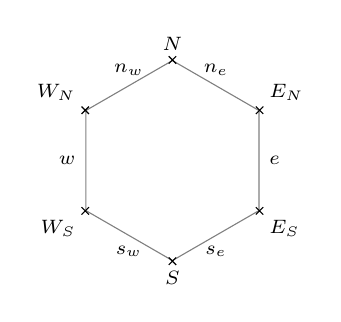
\begin{tikzpicture}[scale=1,transform shape]
%\draw [dashed] (0,0) rectangle (3, -3);
\node (h) [draw, color=gray, shape border rotate=30, minimum size=1in, regular polygon, regular polygon sides=6] at (0,0) {};



\foreach \anchor/\placement/\label in
    {corner 1/above/$N$, corner 2/above left/$W_N$, corner 3/below left/$W_S$, corner 4/below/$S$, corner 5/below right/$E_S$, corner 6/above right/$E_N$}
\draw[shift=(h.\anchor)] plot[mark=x,mark size=1.9pt] coordinates{(0,0)} 
node [\placement] {{\scriptsize\label}};

\foreach \anchor/\placement/\label in
    {side 1/above/$n_w$, side 2/left/$w$, side 3/below/$s_w$, side 4/below/$s_e$, side 5/right/$e$, side 6/above/$n_e$}
\draw[shift=(h.\anchor)] plot coordinates{(0,0)} 
node [\placement] {{\scriptsize\label}};

\end{tikzpicture}\hspace{1cm}
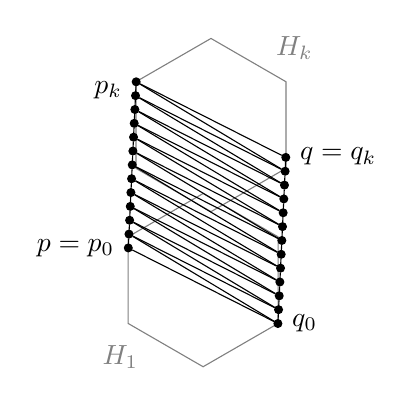
\begin{tikzpicture}[scale=2]

%\draw [color=gray] (0,0) -- (0, 1.22) -- (2.15, 1.22) -- node [right] {\scriptsize $y$}(2.15, 0) -- (0, 0);
\node [draw, color=gray, shape border rotate=30, minimum size=2.2cm, regular polygon, regular polygon sides=6,label=-135:{{\color{gray}{$H_1$}}}] at (0.475,-.2044) (H) {};
\node [draw, color=gray, shape border rotate=30, minimum size=2.2cm, regular polygon, regular polygon sides=6,label=45:{{\color{gray}{$H_k$}}}] at (0.525,.7803) (H) {};


\node at (0, 0) [draw,fill, inner sep = 1pt, circle, label=180:{$p=p_0$}] (h) {};
\node at (0.95, -0.48) [draw,fill, inner sep = 1pt, circle, label=0:{$q_0$}] (l) {};

\draw (h) -- (l);

\foreach \x in {1, ..., 12}
{
  \node at (\x*0.004167, \x*0.0879) [draw, fill, inner sep = 1pt, circle] (h) {};
  \draw (h) -- (l);
  \draw (h) -- (\x*0.004167-0.004167, \x*0.0879-0.0879);
  \node at (\x*0.004167+0.95, \x*0.0879-0.48) [draw,fill, inner sep = 1pt, circle] (l) {};
  \draw (h) -- (l);
  \draw (l) -- (\x*0.004167-0.004167+0.95, \x*0.0879-0.0879-0.48);
}

\node at (0.05, 1) [inner sep = 1pt, circle, label=180:{$p_k$}] {};
\node at (1, 0.58) [inner sep = 1pt, circle, label=0:{$q=q_k$}] (h) {};
%\draw (h) -- (l);

%\draw [color=gray, dashed] (0.15, 3) -- (0.15, 1) -- (2.15, 1) -- (2.15, 3) -- node [below] {\scriptsize $1-\delta$} (0.15, 3);

%\draw [color=gray, dashed] (c2) -- node [above] {\scriptsize $1-\delta$} (0, -1.8) -- (0, 0.2) -- (2.01, 0.2) -- (c2);

\end{tikzpicture}\hspace{0.5cm}
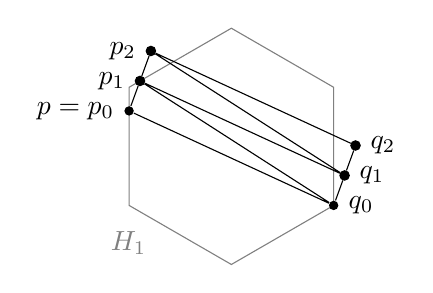
\begin{tikzpicture}[scale=1.5]
%\draw [dashed] (0,0) rectangle (3, -3);
\node [draw, color=gray, shape border rotate=30, minimum size=1.18125in, regular polygon, regular polygon sides=6,label=-135:{{\color{gray}{$H_1$}}}] at (0.866025,-.5) (H) {};


\node at (0,-0.2) [fill, circle, inner sep=1.2pt, label=180:{$p=p_0$}] (a) {};
\path (a) ++(70:0.27) node (p1) [draw,circle,inner sep=1.2pt,fill=black,label=180:$p_1$] {};
\path [draw] (p1) ++(70:0.27) node (p2) [draw,circle,inner sep=1.2pt,fill=black,label=180:$p_2$] {};


\node at (1.73205,-1) [fill, circle, inner sep=1.2pt, label=0:$q_0$] (c2) {};
\path (c2) ++(70:0.27) node (q1) [draw,circle,inner sep=1.2pt,fill=black,label=0:$q_1$] {};
\path (q1) ++(70:0.27) node (q2) [draw,circle,inner sep=1.2pt,fill=black,label=0:$q_2$] {};

\draw (p2) -- (p1) -- (a) -- (c2) -- (p1) -- (q1) -- (p2) -- (q2) -- (q1) -- (c2);

%\draw [color=gray, dashed] (0,0) -- (3,0) -- (3, -3) -- node [below] {\scriptsize $1-\delta$} (0,-3) -- (0, 0);
%\node at (3.2, 0.2) [] {\color{gray}{$S_1$}};
%\draw [dashed] (0.25,0) rectangle (3.25, -3);
%\draw [color=gray, dashed] (0.25,0.7) rectangle (3.25, -2.3);

%\node at (3.25,-2.3) [fill, circle, inner sep=2pt, label=0:$q_1$] (q) {};
%\node at (0.25,0) [fill, circle, inner sep=2pt, label=115:$p_1$] (p1) {};
%\node at (0.5,0.7) [fill, circle, inner sep=2pt, label=115:$p_2$] (p2) {};

%\draw (q) -- (p2) -- (p1) -- (c2) -- (q) -- (p1) -- (a) -- (c2);

%\node at (-0.24,-0.24) [color=gray] {{\small $\delta$}};
\end{tikzpicture}
}


\newcommand{\regular}{
\begin{tikzpicture}[scale=1, transform shape]
\clip (0,-1.14) rectangle (8,3);


\node [color=red!25, shape border rotate=30, minimum size=0.7in, regular polygon, regular polygon sides=6] at (0,0.33) (Hm3) {};

\node [color=blue!25, shape border rotate=30, minimum size=0.58in, regular polygon, regular polygon sides=6] at (0.47,0.45) (Hm2) {};

\node [color=red!25, shape border rotate=30, minimum size=0.78in, regular polygon, regular polygon sides=6] at (1.53,-0.05) (Hm1) {};

\node [draw, color=blue!25, shape border rotate=30, minimum size=0.81in, regular polygon, regular polygon sides=6, label={[label distance=-0.1cm]-120:{\color{blue!25}{$H_1$}}}] at (2,0.77) (H1) {};

\node at (1.7,0.7) {$T_1$};

%\node [draw,color=blue!25, shape border rotate=30, minimum size=0.8in, regular polygon, regular polygon sides=6] at (1.73,0.61) (H1) {};

\node [draw, color=red!25, shape border rotate=30, minimum size=1.2in, regular polygon, regular polygon sides=6, label={[label distance=-0.1cm]120:{\color{red!25}{$H_2$}}}] at (2.93,1.18) (H2) {};

\node at (2.4,1.18) {$T_2$};

\node [draw,color=blue!25, shape border rotate=30, minimum size=1.45in, regular polygon, regular polygon sides=6, label={[label distance=-0.1cm]-60:{\color{blue!25}{$H_3$}}}] at (3.99,0.71) (H3) {};

\node at (3.9,0.75) {$T_3$};

\node [draw, color=red!25, shape border rotate=30, minimum size=1.35in, regular polygon, regular polygon sides=6, label={[label distance=-0.1cm]85:{\color{red!25}{$H_4$}}}] at (4.1,0.9) (H4) {};

\node at (4.85,1.35) {$T_4$};

\node [draw, color=blue!25, shape border rotate=30, minimum size=1in, regular polygon, regular polygon sides=6, label={[label distance=-0.1cm]-30:{\color{blue!25}{$H_5$}}}] at (5.675,1.47) (H5) {};

\node at (5.85,1.5) {$T_5$};

\node [color=red!25, shape border rotate=30, minimum size=1.43in, regular polygon, regular polygon sides=6] at (6.06,3.3) (H6) {};

\node [color=blue!25, shape border rotate=30, minimum size=1.6in, regular polygon, regular polygon sides=6] at (6.25,3.625) (H7) {};

\node [color=red!25, shape border rotate=30, minimum size=1.355in, regular polygon, regular polygon sides=6] at (7.24,3.36) (H8) {};

\node [color=blue!25, shape border rotate=30, minimum size=1.45in, regular polygon, regular polygon sides=6] at (7.6,3.27) (H9) {};

\node [color=red!25, shape border rotate=30, minimum size=1.45in, regular polygon, regular polygon sides=6] at (8,3.5) (H10) {};

\node at (Hm3.side 3) [yshift=.4cm,circle,inner sep=1.4pt] (s) {};

\node at (H10.side 6) [yshift=-3.1cm,circle,inner sep=1.4pt] (t) {};

%\node at (10,3.333) [draw,fill,circle,inner sep=1.4pt,label=180:{$t$}] (t) {};
\draw [gray, dotted] (s) -- (t);

\node at (Hm3.corner 6) (a) {};
\node at (Hm3.corner 1) (b) {};
\node at (Hm2.corner 1) (c) {};
\node at (Hm2.corner 2) (d) {};

\node at (intersection of a--b and c--d) [circle,inner sep=1.4pt] (h1) {};

\node at (Hm2.corner 4) (a) {};
\node at (Hm2.corner 5) (b) {};
\node at (Hm1.corner 2) (c) {};
\node at (Hm1.corner 3) (d) {};

\node at (intersection of a--b and c--d) [circle,inner sep=1.4pt] (l1) {};

\node at (1.11,0.8) [draw,fill,circle,inner sep=1.4pt,label=180:{$u_0$}] (h2) {};

\node at (H1.corner 1) (a) {};
\node at (H1.corner 2) (b) {};
\node at (H2.corner 2) (c) {};
\node at (H2.corner 3) (d) {};

\node at (intersection of a--b and c--d) [draw,fill,circle,inner sep=1.4pt,label=90:{$u_1$}] (h4) {};

\node at (H2.corner 3) (a) {};
\node at (H2.corner 4) (b) {};
\node at (H3.corner 2) (c) {};
\node at (H3.corner 3) (d) {};

\node at (intersection of a--b and c--d) [draw,fill,circle,inner sep=1.4pt,label=-90:{$l_0,l_1,l_2$}] (l3) {};

\node at (3.6,2.32) [draw,fill,circle,inner sep=1.4pt,label=90:{$u_2,u_3$}] (h5) {};

\node at (H4.corner 6) (a) {};
\node at (H4.corner 1) (b) {};
\node at (H5.corner 1) (c) {};
\node at (H5.corner 2) (d) {};

\node at (intersection of a--b and c--d) [draw,fill,circle,inner sep=1.4pt,label=45:{$u_4$}] (h7) {};

\node at (H4.corner 5) (a) {};
\node at (H4.corner 6) (b) {};
\node at (H5.corner 3) (c) {};
\node at (H5.corner 4) (d) {};

\node at (intersection of a--b and c--d) [draw,fill,circle,inner sep=1.4pt,label=-45:{$l_3,l_4,l_5$}] (l6) {};

\node at (6.78,1.9) [draw,fill,circle,inner sep=1.4pt,label=0:{$u_5$}] (l8) {};

\node at (4.48,3.6) [circle,inner sep=1.4pt] (h9) {};

\node at (H8.corner 6) (a) {};
\node at (H8.corner 1) (b) {};
\node at (H9.corner 1) (c) {};
\node at (H9.corner 2) (d) {};

\node at (intersection of a--b and c--d) [circle,inner sep=1.4pt] (h10) {};

\node at (8.34,1.85) [circle,inner sep=1.4pt] (l11) {};


\draw (l3) -- (h2) -- (h4) -- (l3) -- (h5) -- (h4);
\draw (l3) -- (l6) -- (h5) -- (h7) -- (l6) -- (l8) -- (h7); 

\node (tmp) at ($(h7)+(150:5)$) {};
\node (tmp2) at ($(h2)+(90:4)$) {};

\coordinate (z) at (intersection of h7--tmp and h2--tmp2);

%\draw [dashed, red] (h2) -- (z) -- (h7);

\node (tmp) at ($(h7)+(330:5)$) {};
\node (tmp2) at ($(l11)+(270:4)$) {};

\coordinate (z) at (intersection of h7--tmp and l11--tmp2);

%\draw [dashed, red] (l11) -- (z) -- (h7);



\end{tikzpicture}
}



\newcommand{\discretedNdS}{
\begin{tikzpicture}[scale=1]
\clip (-2.5,-1.55) rectangle (6.5,1.55);
\node (h) [draw, color=gray, shape border rotate=30, minimum size=1in, regular polygon, regular polygon sides=6,label={[label distance=-1.5cm]0:{\color{gray}{$H_i$}}}] at (0,0) {};

\node at (h.side 1) [xshift=-0.2cm,yshift=-0.12cm,draw,circle,fill,inner sep=1.4pt,label=90:{\color{blue}{\large +}}] (s1) {};
\node at (h.side 2) [draw,circle,fill,inner sep=1.4pt,label=135:{\color{blue}{\large +}}] (s2) {};
%\node at (h.side 3) [xshift=+0.2cm,yshift=-0.12cm,draw,circle,fill,inner sep=1.4pt,label=90:{\color{blue}{\large +}}] (s3) {};

\draw (s1) -- (h.corner 1) [->,>=stealth',blue,label=-45:{$+$}];
\draw ($(s2) + (-0.1cm,0)$) -- ($(h.corner 2) + (-0.1cm,0.052cm)$) -- ($(h.corner 1) + (0,0.1cm)$) [->,>=stealth',blue,label=-45:{$+$}];
%\draw ($(s3) + (0.052cm,0.1cm)$) -- ($(h.corner 3) + (0.1cm,0.052cm)$) -- ($(h.corner 2) + (0.1cm,-0.052cm)$) -- ($(h.corner 1) + (0,-0.1cm)$) [->,>=stealth',blue,label=-45:{$+$}];

\node at (h.side 6) [draw,circle,fill,inner sep=1.4pt,label=90:{\color{red}{\large --}}] (s1) {};
\node at (h.side 5) [yshift=-0.12cm,draw,circle,fill,inner sep=1.4pt,label=45:{\color{red}{\large --}}] (s2) {};
%\node at (h.side 4) [draw,circle,fill,inner sep=1.4pt,label=90:{\color{red}{\large --}}] (s3) {};

\draw (s1) -- (h.corner 1) [->,>=stealth',red];
\draw ($(s2) + (0.1cm,0)$) -- ($(h.corner 6) + (0.1cm,0.052cm)$) -- ($(h.corner 1) + (0,0.1cm)$) [->,>=stealth',red];
%\draw ($(s3) + (-0.052,0.1cm)$) -- ($(h.corner 5) + (-0.1cm,0.052cm)$) -- ($(h.corner 6) + (-0.1cm,-0.052cm)$) -- ($(h.corner 1) + (0,-0.1cm)$) [->,>=stealth',red];

\node (h) [draw, color=gray, shape border rotate=30, minimum size=1in, regular polygon, regular polygon sides=6,label={[label distance=-1.5cm]0:{\color{gray}{$H_i$}}}] at (5,0) {};

%\node at (h.side 1) [xshift=-0.2cm,yshift=-0.12cm,draw,circle,fill,inner sep=1.4pt,label=-90:{\color{blue}{\large +}}] (s1) {};
\node at (h.side 2) [draw,circle,fill,inner sep=1.4pt,label=-135:{\color{blue}{\large +}}] (s2) {};
\node at (h.side 3) [xshift=+0.2cm,yshift=-0.12cm,draw,circle,fill,inner sep=1.4pt,label=-90:{\color{blue}{\large +}}] (s3) {};

\draw (s3) -- (h.corner 4) [->,>=stealth',blue,label=-45:{$+$}];
\draw ($(s2) + (-0.1cm,0)$) -- ($(h.corner 3) + (-0.1cm,-0.052cm)$) -- ($(h.corner 4) + (0,-0.1cm)$) [->,>=stealth',blue,label=-45:{$+$}];
%\draw ($(s1) + (0.052cm,-0.09cm)$) -- ($(h.corner 2) + (0.1cm,-0.052cm)$) -- ($(h.corner 3) + (0.1cm,0.052cm)$) -- ($(h.corner 4) + (0,0.1cm)$) [->,>=stealth',blue,label=-45:{$+$}];

%\node at (h.side 6) [draw,circle,fill,inner sep=1.4pt,label=-90:{\color{red}{\large --}}] (s1) {};
\node at (h.side 5) [yshift=-0.12cm,draw,circle,fill,inner sep=1.4pt,label=-45:{\color{red}{\large --}}] (s2) {};
\node at (h.side 4) [draw,circle,fill,inner sep=1.4pt,label=-90:{\color{red}{\large --}}] (s3) {};

\draw (s3) -- (h.corner 4) [->,>=stealth',red];
\draw ($(s2) + (0.1cm,0)$) -- ($(h.corner 5) + (0.1cm,-0.052cm)$) -- ($(h.corner 4) + (0,-0.1cm)$) [->,>=stealth',red];
%\draw ($(s1) + (-0.052,-0.1cm)$) -- ($(h.corner 6) + (-0.1cm,-0.052cm)$) -- ($(h.corner 5) + (-0.1cm,0.052cm)$) -- ($(h.corner 4) + (0,0.1cm)$) [->,>=stealth',red];
\end{tikzpicture}\hspace{1.34cm}
\begin{tikzpicture}[scale=1]
\clip (-2.35,-1.45) rectangle (6.5,1.65);
\node (h) [draw, color=gray, shape border rotate=30, minimum size=1in, regular polygon, regular polygon sides=6,label={[label distance=-1.5cm]0:{\color{gray}{$H_i$}}}] at (0,0) {};

\node at (h.side 2) [draw,circle,fill,inner sep=1.4pt,label=180:{$u_{i-1}$}] (uj) {};
\node at (h.side 6) [draw,circle,fill,inner sep=1.4pt,label=0:{$u_i$}] (ujp) {};

\draw (uj) -- (h.corner 2) -- (h.corner 1) [->,>=stealth',blue];
\draw (ujp) -- (h.corner 1) [->,>=stealth',red];

\draw (uj) -- (ujp);

\node at (-1.45,1.1) [blue] {$p_N(u_{i-1},i)$};
\node at (1.05,1.45) [red] {$p_N(u_i,i)$};
\end{tikzpicture}
}



\newcommand{\definitions}{
\begin{tikzpicture}[scale=1, transform shape]
\clip (-2.2,-1.14) rectangle (12,5.66);


\node [draw, color=red!25, shape border rotate=30, minimum size=0.7in, regular polygon, regular polygon sides=6] at (0,0.33) (Hm3) {};

\node [draw, color=blue!25, shape border rotate=30, minimum size=0.58in, regular polygon, regular polygon sides=6] at (0.47,0.45) (Hm2) {};

\node [draw,color=red!25, shape border rotate=30, minimum size=0.78in, regular polygon, regular polygon sides=6] at (1.53,-0.05) (Hm1) {};

\node [draw, color=blue!25, shape border rotate=30, minimum size=0.81in, regular polygon, regular polygon sides=6] at (2,0.77) (H1) {};

%\node [draw,color=blue!25, shape border rotate=30, minimum size=0.8in, regular polygon, regular polygon sides=6] at (1.73,0.61) (H1) {};

\node [draw, color=red!25, shape border rotate=30, minimum size=1.2in, regular polygon, regular polygon sides=6] at (2.93,1.18) (H2) {};

\node [draw,color=blue!25, shape border rotate=30, minimum size=1.45in, regular polygon, regular polygon sides=6] at (3.99,0.71) (H3) {};

\node [draw, color=red!25, shape border rotate=30, minimum size=1.35in, regular polygon, regular polygon sides=6] at (4.1,0.9) (H4) {};

\node [draw, color=blue!25, shape border rotate=30, minimum size=1in, regular polygon, regular polygon sides=6] at (5.675,1.47) (H5) {};

\node [draw,color=red!25, shape border rotate=30, minimum size=1.43in, regular polygon, regular polygon sides=6] at (6.06,3.3) (H6) {};

\node [draw,color=blue!25, shape border rotate=30, minimum size=1.6in, regular polygon, regular polygon sides=6] at (6.25,3.625) (H7) {};

\node [draw,color=red!25, shape border rotate=30, minimum size=1.355in, regular polygon, regular polygon sides=6] at (7.24,3.36) (H8) {};

\node [draw,color=blue!25, shape border rotate=30, minimum size=1.45in, regular polygon, regular polygon sides=6] at (7.6,3.27) (H9) {};

\node [draw, color=red!25, shape border rotate=30, minimum size=1.45in, regular polygon, regular polygon sides=6] at (8,3.5) (H10) {};



\node at (Hm3.side 2) [yshift=-0.32cm,draw,circle,fill,inner sep=1.4pt,label=180:{$u_0,l_0,s$}] (s) {};

\node at (H10.side 5) [yshift=-0.6cm,draw,circle,fill,inner sep=1.4pt,label=0:{$t,u_{12},l_{12}$}] (t) {};

%\node at (10,3.333) [draw,fill,circle,inner sep=1.4pt,label=180:{$t$}] (t) {};
\draw [gray, dotted] (s) -- (t);

\node at (Hm3.corner 6) (a) {};
\node at (Hm3.corner 1) (b) {};
\node at (Hm2.corner 1) (c) {};
\node at (Hm2.corner 2) (d) {};

\node at (intersection of a--b and c--d) [draw,fill,circle,inner sep=1.4pt,label=90:{$u_1$}] (h1) {};

\node at (Hm2.corner 4) (a) {};
\node at (Hm2.corner 5) (b) {};
\node at (Hm1.corner 2) (c) {};
\node at (Hm1.corner 3) (d) {};

\node at (intersection of a--b and c--d) [draw,fill,circle,inner sep=1.4pt,label=-90:{$l_1,l_2$}] (l1) {};

\node at (1.11,0.7) [draw,fill,circle,inner sep=1.4pt,label=90:{$u_2,u_3$}] (h2) {};

\node at (H1.corner 1) (a) {};
\node at (H1.corner 2) (b) {};
\node at (H2.corner 2) (c) {};
\node at (H2.corner 3) (d) {};

\node at (intersection of a--b and c--d) [draw,fill,circle,inner sep=1.4pt,label=90:{$u_4$}] (h4) {};

\node at (H2.corner 3) (a) {};
\node at (H2.corner 4) (b) {};
\node at (H3.corner 2) (c) {};
\node at (H3.corner 3) (d) {};

\node at (intersection of a--b and c--d) [draw,fill,circle,inner sep=1.4pt,label=-90:{$l_3,l_4,l_5$}] (l3) {};

\node at (3.6,2.32) [draw,fill,circle,inner sep=1.4pt,label=90:{$u_5,u_6$}] (h5) {};

\node at (H4.corner 6) (a) {};
\node at (H4.corner 1) (b) {};
\node at (H5.corner 1) (c) {};
\node at (H5.corner 2) (d) {};

\node at (intersection of a--b and c--d) [draw,fill,circle,inner sep=1.4pt,label=45:{$u_7,u_8$}] (h7) {};

\node at (H4.corner 5) (a) {};
\node at (H4.corner 6) (b) {};
\node at (H5.corner 3) (c) {};
\node at (H5.corner 4) (d) {};

\node at (intersection of a--b and c--d) [draw,fill,circle,inner sep=1.4pt,label=-45:{$l_6,l_7$}] (l6) {};

\node at (6.78,1.9) [draw,fill,circle,inner sep=1.4pt,label=-90:{$l_8,l_9,l_{10}$}] (l8) {};

\node at (4.48,3.6) [draw,fill,circle,inner sep=1.4pt,label=180:{$u_9$}] (h9) {};

\node at (H8.corner 6) (a) {};
\node at (H8.corner 1) (b) {};
\node at (H9.corner 1) (c) {};
\node at (H9.corner 2) (d) {};

\node at (intersection of a--b and c--d) [draw,fill,circle,inner sep=1.4pt,label=90:{$u_{10},u_{11}$}] (h10) {};

\node at (8.34,1.85) [draw,fill,circle,inner sep=1.4pt,label=-45:{$l_{11}$}] (l11) {};


\draw (h1) -- (s) -- (l1) -- (h1) -- (h2) -- (l1) -- (l3) -- (h2) -- (h4) -- (l3) -- (h5) -- (h4);
\draw (l3) -- (l6) -- (h5) -- (h7) -- (l6) -- (l8) -- (h7) -- (h9) -- (l8) -- (h10) -- (h9);
\draw (l8) -- (l11) -- (h10) -- (t) -- (l11); 

\node (tmp) at ($(h7)+(150:5)$) {};
\node (tmp2) at ($(h2)+(90:4)$) {};

\coordinate (z) at (intersection of h7--tmp and h2--tmp2);

\draw [dashed, red] (h2) -- (z) -- (h7);


\node (tmp) at ($(h4)+(150:5)$) {};
\coordinate (z) at (intersection of h4--tmp and h2--tmp2);
\draw [dotted, red] (h4) -- (z) -- (h2);

\node (tmp) at ($(h5)+(150:5)$) {};
\node (tmp2) at ($(h4)+(90:5)$) {};
\coordinate (z) at (intersection of h5--tmp and h4--tmp2);
\draw [dotted, red] (h4) -- (z) -- (h5);

\node (tmp) at ($(h7)+(150:5)$) {};
\node (tmp2) at ($(h5)+(90:5)$) {};
\coordinate (z) at (intersection of h7--tmp and h5--tmp2);
\draw [dotted, red] (h7) -- (z) -- (h5);




%%%%%%

\node (tmp) at ($(h7)+(330:5)$) {};
\node (tmp2) at ($(l11)+(270:4)$) {};

\coordinate (z) at (intersection of h7--tmp and l11--tmp2);

\draw [dashed, red] (l11) -- (z) -- (h7);


\node (tmp2) at ($(l8)+(270:5)$) {};
\coordinate (z) at (intersection of h7--tmp and l8--tmp2);
\draw [dotted, red] (l8) -- (z) -- (h7);

\node (tmp) at ($(l8)+(330:5)$) {};
\node (tmp2) at ($(l11)+(270:5)$) {};
\coordinate (z) at (intersection of l8--tmp and l11--tmp2);
\draw [dotted, red] (l8) -- (z) -- (l11);




\end{tikzpicture}
}




\newcommand{\infity}{
\begin{tikzpicture}[scale=1, transform shape]
\clip (0,-1.14) rectangle (8,3);


\node [color=red!25, shape border rotate=30, minimum size=0.7in, regular polygon, regular polygon sides=6] at (0,0.33) (Hm3) {};

\node [color=blue!25, shape border rotate=30, minimum size=0.58in, regular polygon, regular polygon sides=6] at (0.47,0.45) (Hm2) {};

\node [color=red!25, shape border rotate=30, minimum size=0.78in, regular polygon, regular polygon sides=6] at (1.53,-0.05) (Hm1) {};

\node [draw, color=blue!25, shape border rotate=30, minimum size=0.81in, regular polygon, regular polygon sides=6, label={[label distance=-0.1cm]-120:{\color{blue!25}{$H_1$}}}] at (2,0.77) (H1) {};

\node at (1.7,0.7) {$T_1$};

%\node [draw,color=blue!25, shape border rotate=30, minimum size=0.8in, regular polygon, regular polygon sides=6] at (1.73,0.61) (H1) {};

\node [draw, color=red!25, shape border rotate=30, minimum size=1.2in, regular polygon, regular polygon sides=6, label={[label distance=-0.1cm]120:{\color{red!25}{$H_2$}}}] at (2.93,1.18) (H2) {};

\node at (2.4,1.18) {$T_2$};

\node [draw,color=blue!25, shape border rotate=30, minimum size=1.45in, regular polygon, regular polygon sides=6, label={[label distance=-0.1cm]-60:{\color{blue!25}{$H_3$}}}] at (3.99,0.71) (H3) {};

\node at (3.9,0.75) {$T_3$};

\node [draw, color=red!25, shape border rotate=30, minimum size=1.35in, regular polygon, regular polygon sides=6, label={[label distance=-0.1cm]85:{\color{red!25}{$H_4$}}}] at (4.1,0.9) (H4) {};

\node at (4.85,1.35) {$T_4$};

\node [draw, color=blue!25, shape border rotate=30, minimum size=1in, regular polygon, regular polygon sides=6, label={[label distance=-0.1cm]-30:{\color{blue!25}{$H_5$}}}] at (5.675,1.47) (H5) {};

\node at (5.85,1.5) {$T_5$};

\node [color=red!25, shape border rotate=30, minimum size=1.43in, regular polygon, regular polygon sides=6] at (6.06,3.3) (H6) {};

\node [color=blue!25, shape border rotate=30, minimum size=1.6in, regular polygon, regular polygon sides=6] at (6.25,3.625) (H7) {};

\node [color=red!25, shape border rotate=30, minimum size=1.355in, regular polygon, regular polygon sides=6] at (7.24,3.36) (H8) {};

\node [color=blue!25, shape border rotate=30, minimum size=1.45in, regular polygon, regular polygon sides=6] at (7.6,3.27) (H9) {};

\node [color=red!25, shape border rotate=30, minimum size=1.45in, regular polygon, regular polygon sides=6] at (8,3.5) (H10) {};

\node at (Hm3.side 2) [yshift=-0.32cm,circle,inner sep=1.4pt] (s) {};

\node at (H10.side 5) [yshift=-0.6cm,circle,inner sep=1.4pt] (t) {};

\draw [gray, dotted] (s) -- (t);

\node at (Hm3.corner 6) (a) {};
\node at (Hm3.corner 1) (b) {};
\node at (Hm2.corner 1) (c) {};
\node at (Hm2.corner 2) (d) {};

\node at (intersection of a--b and c--d) [circle,inner sep=1.4pt] (h1) {};

\node at (Hm2.corner 4) (a) {};
\node at (Hm2.corner 5) (b) {};
\node at (Hm1.corner 2) (c) {};
\node at (Hm1.corner 3) (d) {};

\node at (intersection of a--b and c--d) [circle,inner sep=1.4pt] (l1) {};

\node at (1.11,0.7) [draw,fill,circle,inner sep=1.4pt,label=180:{$u_0$}] (h2) {};

\node at (H1.corner 1) (a) {};
\node at (H1.corner 2) (b) {};
\node at (H2.corner 2) (c) {};
\node at (H2.corner 3) (d) {};

\node at (intersection of a--b and c--d) [draw,fill,circle,inner sep=1.4pt,label=90:{$u_1$}] (h4) {};

\node at (H2.corner 3) (a) {};
\node at (H2.corner 4) (b) {};
\node at (H3.corner 2) (c) {};
\node at (H3.corner 3) (d) {};

\node at (intersection of a--b and c--d) [draw,fill,circle,inner sep=1.4pt,label=-90:{$l_0,l_1,l_2$}] (l3) {};

\node at (3.6,2.32) [draw,fill,circle,inner sep=1.4pt,label=90:{$u_2,u_3$}] (h5) {};

\node at (H4.corner 6) (a) {};
\node at (H4.corner 1) (b) {};
\node at (H5.corner 1) (c) {};
\node at (H5.corner 2) (d) {};

\node at (intersection of a--b and c--d) [draw,fill,circle,inner sep=1.4pt,label=45:{$u_4,u_5$}] (h7) {};

\node at (H4.corner 5) (a) {};
\node at (H4.corner 6) (b) {};
\node at (H5.corner 3) (c) {};
\node at (H5.corner 4) (d) {};

\node at (intersection of a--b and c--d) [draw,fill,circle,inner sep=1.4pt,label=-45:{$l_3,l_4$}] (l6) {};

\node at (6.78,1.9) [draw,fill,circle,inner sep=1.4pt,label=0:{$l_5$}] (l8) {};

\node at (4.48,3.6) [circle,inner sep=1.4pt] (h9) {};

\node at (H8.corner 6) (a) {};
\node at (H8.corner 1) (b) {};
\node at (H9.corner 1) (c) {};
\node at (H9.corner 2) (d) {};

\node at (intersection of a--b and c--d) [circle,inner sep=1.4pt] (h10) {};

\node at (8.34,1.85) [circle,inner sep=1.4pt] (l11) {};


\draw (l3) -- (h2) -- (h4) -- (l3) -- (h5) -- (h4);
\draw (l3) -- (l6) -- (h5) -- (h7) -- (l6) -- (l8) -- (h7); 

\node (tmp) at ($(h7)+(150:5)$) {};
\node (tmp2) at ($(h2)+(90:4)$) {};

\coordinate (z) at (intersection of h7--tmp and h2--tmp2);

%\draw [dashed, red] (h2) -- (z) -- (h7);

\node (tmp) at ($(h7)+(330:5)$) {};
\node (tmp2) at ($(l11)+(270:4)$) {};

\coordinate (z) at (intersection of h7--tmp and l11--tmp2);

%\draw [dashed, red] (l11) -- (z) -- (h7);



\end{tikzpicture}
}

\newcommand{\infinity}{
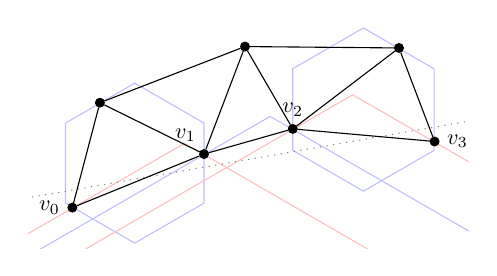
\begin{tikzpicture}[scale=.8, transform shape]
\clip (-0.2,-0.2) rectangle (6.8,3.3);


\node [draw, color=blue!25, shape border rotate=30, minimum size=1in, regular polygon, regular polygon sides=6] at (1.5,1.15) (H1) {};

\node [draw, color=red!25, shape border rotate=30, minimum size=3.2in, regular polygon, regular polygon sides=6] at (2.29,-2.6) (H2) {};

\node [draw,color=blue!25, shape border rotate=30, minimum size=4.45in, regular polygon, regular polygon sides=6] at (3.65,-3.76) (H3) {};

\node [draw, color=red!25, shape border rotate=30, minimum size=5.35in, regular polygon, regular polygon sides=6] at (4.96,-4.56) (H4) {};

\node [draw, color=blue!25, shape border rotate=30, minimum size=1.02in, regular polygon, regular polygon sides=6] at (5.13,2) (H5) {};

\node at (H1.corner 3) [xshift=-1.1cm,inner sep=1.4pt,label=180:{$s$}] (s) {};

\node at (H5.side 5) [xshift=+1.6cm,yshift=+0cm,inner sep=1.4pt,label=0:{$t,u_{12},l_{12}$}] (t) {};

\draw [gray, dotted] (s) -- (t);

\node at (H1.corner 3) (a) {};
\node at (H1.corner 4) (b) {};
\node at (H2.corner 1) (c) {};
\node at (H2.corner 2) (d) {};

\node at (intersection of a--b and c--d) [draw,fill,circle,inner sep=1.4pt,label=180:{$v_0$}] (v0) {};

\node at (H2.corner 1) (a) {};
\node at (H2.corner 6) (b) {};
\node at (H3.corner 1) (c) {};
\node at (H3.corner 2) (d) {};

\node at (intersection of a--b and c--d) [draw,fill,circle,inner sep=1.4pt,label=94:{$v_1$}] (v1) {};

\node at (H3.corner 1) (a) {};
\node at (H3.corner 6) (b) {};
\node at (H4.corner 1) (c) {};
\node at (H4.corner 2) (d) {};

\node at (intersection of a--b and c--d) [draw,fill,circle,inner sep=1.4pt,label=92:{$v_2$}] (v2) {};

\node at (H4.corner 1) (a) {};
\node at (H4.corner 6) (b) {};
\node at (H5.corner 5) (c) {};
\node at (H5.corner 6) (d) {};

\node at (intersection of a--b and c--d) [draw,fill,circle,inner sep=1.4pt,label=0:{$v_3$}] (v3) {};

\node at (H1.side 1) [draw,fill,circle,inner sep=1.4pt] (v) {};
\node at (H5.side 6) [draw,fill,circle,inner sep=1.4pt] (w) {};

\node at (3.25,3) [draw,fill,circle,inner sep=1.4pt] (u) {};


\draw (v1) -- (v) -- (v0) -- (v1) -- (v2) -- (v3) -- (w) -- (v2);

\draw (v) -- (u) -- (w); 
\draw (v1) -- (u) -- (v2); 

\end{tikzpicture}\hspace{1.5cm}
\begin{tikzpicture}[scale=.8, transform shape]
\clip (-0.2,-0.2) rectangle (6.8,3.3);


\node [draw, color=blue!25, shape border rotate=30, minimum size=1in, regular polygon, regular polygon sides=6] at (1.5,1.15) (H1) {};

\node [draw, color=red!25, shape border rotate=30, minimum size=3.2in, regular polygon, regular polygon sides=6] at (2.29,-2.6) (H2) {};

\node [draw,color=blue!25, shape border rotate=30, minimum size=4.45in, regular polygon, regular polygon sides=6] at (3.65,-3.76) (H3) {};

\node [draw, color=red!25, shape border rotate=30, minimum size=5.35in, regular polygon, regular polygon sides=6] at (4.96,-4.56) (H4) {};

\node [draw, color=blue!25, shape border rotate=30, minimum size=1.02in, regular polygon, regular polygon sides=6] at (5.13,2) (H5) {};

\node at (H1.corner 3) [xshift=-1.1cm,inner sep=1.4pt,label=180:{$s$}] (s) {};

\node at (H5.side 5) [xshift=+1.6cm,yshift=+0cm,inner sep=1.4pt,label=0:{$t,u_{12},l_{12}$}] (t) {};

\draw [gray, dotted] (s) -- (t);

\node at (H1.corner 3) (a) {};
\node at (H1.corner 4) (b) {};
\node at (H2.corner 1) (c) {};
\node at (H2.corner 2) (d) {};

\node at (intersection of a--b and c--d) [draw,fill,circle,inner sep=1.4pt,label=180:{$v_0$}] (v0) {};

\node at (H2.corner 1) (a) {};
\node at (H2.corner 6) (b) {};
\node at (H3.corner 1) (c) {};
\node at (H3.corner 2) (d) {};

\node at (intersection of a--b and c--d) [draw,fill,circle,inner sep=1.4pt,label=95:{$v_1$}] (v1) {};

\node at (H3.corner 1) (a) {};
\node at (H3.corner 6) (b) {};
\node at (H4.corner 1) (c) {};
\node at (H4.corner 2) (d) {};

\node at (intersection of a--b and c--d) [draw,fill,circle,inner sep=1.4pt,label=95:{$v_2$}] (v2) {};

\node at (H4.corner 1) (a) {};
\node at (H4.corner 6) (b) {};
\node at (H5.corner 5) (c) {};
\node at (H5.corner 6) (d) {};

\node at (intersection of a--b and c--d) [draw,fill,circle,inner sep=1.4pt,label=0:{$v_3$}] (v3) {};

\node at (H1.side 1) [draw,fill,circle,inner sep=1.4pt] (v) {};
\node at (H5.side 6) [draw,fill,circle,inner sep=1.4pt] (w) {};

%\node at (3.25,3) [draw,fill,circle,inner sep=1.4pt] (u) {};



\draw (v1) -- (v) -- (v0) -- (v1) -- (v2) -- (v3) -- (w) -- (v2);

%\draw (v) -- (u) -- (w); 
%\draw (v1) -- (u) -- (v2); 

\draw (v0) -- ($(v0)+(-90:4)$);
\draw (v1) -- ($(v1)+(-90:4)$);
\draw (v2) -- ($(v2)+(-90:4)$);
\draw (v3) -- ($(v3)+(-90:4)$);

\end{tikzpicture}
}



\newcommand{\caseA}{
\begin{tikzpicture}[scale=.9, transform shape]
\clip (-0.3,-0.8) rectangle (10,4.3);

\coordinate (t) at (10,3.333);
\coordinate (s) at (0,0);
\draw [gray, dotted] (s) -- (t);



\node [draw, gray!25, shape border rotate=30, minimum size=0.58in, regular polygon, regular polygon sides=6] at (0.47,0.45) (Hm2) {};

\node [color=gray!50, dashed, shape border rotate=30, minimum size=0.78in, regular polygon, regular polygon sides=6] at (1.53,-0.05) (Hm1) {};

\node [draw, color=red!25, shape border rotate=30, minimum size=0.81in, regular polygon, regular polygon sides=6] at (2,0.77) (H0) {};

\node [color=gray!50, shape border rotate=30, minimum size=0.8in, regular polygon, regular polygon sides=6] at (1.73,0.61) (H1) {};

\node [draw, color=red!25, shape border rotate=30, minimum size=1.2in, regular polygon, regular polygon sides=6] at (2.93,1.18) (H2) {};

\node [color=gray!50, shape border rotate=30, minimum size=1.45in, regular polygon, regular polygon sides=6] at (3.99,0.71) (H3) {};

\node [draw, color=red!25, shape border rotate=30, minimum size=1.35in, regular polygon, regular polygon sides=6] at (4.1,0.9) (H4) {};

\node [draw, color=blue!25, shape border rotate=30, minimum size=1in, regular polygon, regular polygon sides=6] at (5.675,1.47) (H5) {};

\node [color=gray!50, shape border rotate=30, minimum size=0.906in, regular polygon, regular polygon sides=6] at (5.775,2.27) (H6) {};

\node [draw, color=gray!25, shape border rotate=30, minimum size=0.906in, regular polygon, regular polygon sides=6] at (10.37,2.8) (H7) {};

%\node at (H0.corner 4) (a) {};
%\node at (H0.corner 5) (b) {};
%\node at (H1.corner 2) (c) {};
%\node at (H1.corner 3) (d) {};

%\node at (intersection of a--b and c--d) [draw,fill,circle,inner sep=1.4pt] (l1) {};

\node at (1.11,0.7) [draw,fill,circle,inner sep=1.4pt,label=180:{$p=u_{r'}$}] (h0) {};

\node at (H1.corner 1) (a) {};
\node at (H1.corner 2) (b) {};
\node at (H2.corner 2) (c) {};
\node at (H2.corner 3) (d) {};

\node at (intersection of a--b and c--d) [draw,fill,circle,inner sep=1.4pt,label=-4:{$u_{r'+1}$}] (h1h2) {};

\node at (H2.corner 3) (a) {};
\node at (H2.corner 4) (b) {};
\node at (H3.corner 2) (c) {};
\node at (H3.corner 3) (d) {};

\node at (intersection of a--b and c--d) [draw,fill,circle,inner sep=1.4pt] (l2l3) {};

\node at (3.6,2.32) [draw,fill,circle,inner sep=1.4pt,label=177:{$u_{r-1}$}] (h3h4) {};

\node at (H4.corner 6) (a) {};
\node at (H4.corner 1) (b) {};
\node at (H5.corner 1) (c) {};
\node at (H5.corner 2) (d) {};

\node at (intersection of a--b and c--d) [draw,fill,circle,inner sep=1.4pt,label=90:{$u_r$}] (h5h6) {};

\node at (6.78,1.9) [draw,fill,circle,inner sep=1.4pt,label=0:{$l_s$}] (l6) {};

\node at (H4.corner 5) (a) {};
\node at (H4.corner 6) (b) {};
\node at (H5.corner 3) (c) {};
\node at (H5.corner 4) (d) {};

\node at (intersection of a--b and c--d) [draw,fill,circle,inner sep=1.4pt] (l4l5) {};

\node (tmp) at ($(h3h4)+(90:4)$) {};
\node (tmp2) at ($(h5h6)+(150:4)$) {};

\coordinate (z3) at (intersection of h3h4--tmp and h5h6--tmp2);

\node (tmp) at ($(h3h4)+(150:4)$) {};
\node (tmp2) at ($(h1h2)+(90:4)$) {};

\coordinate (z2) at (intersection of h3h4--tmp and h1h2--tmp2);

\node (tmp) at ($(h1h2)+(150:4)$) {};
\node (tmp2) at ($(h0)+(90:4)$) {};

\coordinate (z1) at (intersection of h1h2--tmp and h0--tmp2);

\draw [dashed, red] (h5h6) -- (z3) -- (h3h4) -- (z2) -- (h1h2) -- (z1) -- (h0);
%\draw [dashed, red] (h3h4) -- (z2);
%\draw [dashed, red] (h1h2) -- (z1);

\node (tmp) at ($(h5h6)+(150:5)$) {};
\node (tmp2) at ($(h0)+(90:4)$) {};

\coordinate (z) at (intersection of h5h6--tmp and h1h2--tmp2);

\draw [dotted, red] (h5h6) -- (z) -- (h0);


%\node at (H5.corner 5) (a) {};
%\node at (H5.corner 6) (b) {};
%\node at (H6.corner 4) (c) {};
%\node at (H6.corner 5) (d) {};

%\node at (intersection of a--b and c--d) [draw,fill,circle,inner sep=1.4pt,label=270:{$l_5$}] (l5) {};




\draw [thick,red] (h0) -- (h1h2) -- (h3h4) -- (h5h6);
\draw (h0) -- (l2l3);
\draw (h1h2) -- (l2l3) -- (h1h2);
\draw (h3h4) -- (l2l3) -- (l4l5) -- (h3h4);
\draw (h5h6) -- (l4l5) -- (l6);
\draw [thick, blue] (l6) -- (h5h6);
%\draw (h3) -- (l4) -- (h1);


\coordinate (tmp) at ($(h5h6)+(-30:8)$);
\coordinate (tmp2) at ($(l6)+(-90:6)$);

\coordinate (z4) at (intersection of h5h6--tmp and l6--tmp2);

\draw [dashed, blue] (h5h6) -- (z4) -- (l6);

\coordinate (tmp) at ($(l6)+(-30:3)$);
\node at ($(tmp)+(90:2.25)$) [draw,fill,circle,inner sep=1.4pt,label=-135:{$l_{s'}=q$}] (tmp2) {};


\coordinate (tmp3) at ($(z4)+(-30:6)$);
\coordinate (tmp4) at ($(tmp)+(-90:4)$);

\coordinate (z5) at (intersection of z4--tmp3 and tmp--tmp4);

\draw [dotted, red] (h5h6) -- (z5) -- (tmp2);

\draw [dashed, red] (l6) -- (tmp) -- (tmp2);
\end{tikzpicture}
}





\def\tikzbox{
\clip (-0.42,-1.5) rectangle (4.05,3);
%\node at (0,0)  (s) [draw,fill,circle,inner sep=2pt,label=180:{$s$}] {};
\coordinate (t) at (4,2.5);
\coordinate (s) at (-.5,0);
%\node [draw, color=gray, shape border rotate=30, minimum size=1in, regular polygon, regular polygon sides=6] at (1.1,0) (H1) {};


%\draw [shift=(H1.side 2)] plot[mark=*,mark size=1.9pt] coordinates{(0,0)} 
%node [left] (s) {{$s$}};

%\node [draw, color=gray, dashed, shape border rotate=30, minimum size=1.3in, regular polygon, regular polygon sides=6] at (1.8,.5) (H2) {};

%\node at (H1.corner 1) (a) {};
%\node at (H1.corner 2) (b) {};
%\node at (H2.corner 2) (c) {};
%\node at (H2.corner 3) (d) {};

%\node at (intersection of a--b and c--d) [draw,fill,circle,inner sep=1.4pt,label=175:{$u_1$}] (h1) {};

\node [transform shape,draw, color=red!25, shape border rotate=30, minimum size=0.7in, regular polygon, regular polygon sides=6] at (0.51,1.2) (H0) {};

%\node at (H0.side 3) [draw, circle, fill, inner sep=1.4pt,label=180:$s$] {};

\node at (0.16,0.51) [transform shape,inner sep=1.4pt, draw,circle,fill=red,label=180:{$u_r$}] (h0) {};

\draw [gray, dotted] (s) -- (t);


\node [transform shape,draw, color=blue!25, shape border rotate=30, minimum size=0.8in, regular polygon, regular polygon sides=6] at (.87,1.35) (H1) {};

\node [draw, color=red!25, shape border rotate=30, minimum size=0.95in, regular polygon, regular polygon sides=6] at (1.2,1.35) (H2) {};

\node [draw, color=blue!25, shape border rotate=30, minimum size=0.95in, regular polygon, regular polygon sides=6] at (1.3,1.41) (H3) {};

\node [draw, color=red!25, shape border rotate=30, minimum size=0.75in, regular polygon, regular polygon sides=6] at (1.74,1.41) (H4) {};

\node [draw, color=blue!25, shape border rotate=30, minimum size=0.685in, regular polygon, regular polygon sides=6] at (1.96,1.53) (H5) {};

\node [draw, color=red!25, shape border rotate=30, minimum size=0.6in, regular polygon, regular polygon sides=6] at (2.9,1.59) (H6) {};

%\node [draw, color=gray!50, shape border rotate=30, minimum size=0.906in, regular polygon, regular polygon sides=6] at (10.37,2.8) (H7) {};

\node at (H0.corner 4) (a) {};
\node at (H0.corner 5) (b) {};
\node at (H1.corner 3) (c) {};
\node at (H1.corner 4) (d) {};

\node at (intersection of a--b and c--d) [transform shape,draw,fill,circle,inner sep=1.4pt,label=270:{$l_{r+1}$}] (l1) {};

\node at (H0.corner 1) (az) {};
\node at (H0.corner 2) (bz) {};
\node at (H1.corner 2) (cz) {};
\node at (H1.corner 3) (dz) {};

\node at (intersection of az--bz and cz--dz) [transform shape,draw,fill,circle,inner sep=1.4pt] (h1) {};


\node at (.47,2.14) [draw,fill,circle,inner sep=1.4pt] (h2) {};

\node at (2.02,0.62) [draw,fill,circle,inner sep=1.4pt] (l2) {};

\node at (1.82,2.32) [draw,fill,circle,inner sep=1.4pt] (h3) {};

\node at (2.57,1.02) [draw,fill,circle,inner sep=1.4pt] (l3) {};

\node at (2.47,2.1) [transform shape,draw,fill,circle,inner sep=1.4pt,label=90:{$u_{s-1}$}] (h4) {};

\node at (3.45,2.03) [transform shape,draw,fill=red,circle,inner sep=1.4pt,label=0:{$l_s$}] (l4) {};


%\node at (H1.corner 1) (a) {};
%\node at (H1.corner 2) (b) {};
%\node at (H2.corner 2) (c) {};
%\node at (H2.corner 3) (d) {};

%\node at (intersection of a--b and c--d) [draw,fill,circle,inner sep=1.4pt,label=180:{$u_{r'}$}] (h1h2) {};

%\node at (H2.corner 3) (a) {};
%\node at (H2.corner 4) (b) {};
%\node at (H3.corner 2) (c) {};
%\node at (H3.corner 3) (d) {};

%\node at (intersection of a--b and c--d) [draw,fill,circle,inner sep=1.4pt] (l2l3) {};


%\node at (H4.corner 6) (a) {};
%\node at (H4.corner 1) (b) {};
%\node at (H5.corner 1) (c) {};
%\node at (H5.corner 2) (d) {};

%\node at (intersection of a--b and c--d) [draw,fill,circle,inner sep=1.4pt,label=45:{$u_r$}] (h5h6) {};

%\node at (6.78,1.9) [draw,fill,circle,inner sep=1.4pt,label=45:{$l_s$}] (l6) {};

%\node at (H4.corner 5) (a) {};
%\node at (H4.corner 6) (b) {};
%\node at (H5.corner 3) (c) {};
%\node at (H5.corner 4) (d) {};

%\node at (intersection of a--b and c--d) [draw,fill,circle,inner sep=1.4pt] (l4l5) {};

%\node (tmp) at ($(h0)+(90:10)$) [transform shape] {};
%\node (tmp2) at ($(l4)+(150:10)$) [transform shape] {};

%\coordinate (z) at (intersection of h0--tmp and l4--tmp2);
\coordinate (z) at (3.45, -1.39);

%\node (tmp) at ($(h3h4)+(150:4)$) {};
%\node (tmp2) at ($(h1h2)+(90:4)$) {};

%\coordinate (z2) at (intersection of h3h4--tmp and h1h2--tmp2);

\draw [transform shape, dashed, red] (h0) -- (z);
\draw [transform shape, dashed, red] (l4) -- (z);

%\node (tmp) at ($(h5h6)+(150:4)$) {};
%\node (tmp2) at ($(h1h2)+(90:3)$) {};

%\coordinate (z3) at (intersection of h5h6--tmp and h1h2--tmp2);

%\draw [dashed, red] (h5h6) -- (z3) -- (h1h2);

%\draw [thick,red] (h1h2) -- (h3h4) -- (h5h6);

%\draw (h1h2) -- (l1) -- (l2l3) -- (h1h2);
%\draw (h3h4) -- (l2l3) -- (l4l5) -- (h3h4);
%\draw (h5h6) -- (l4l5) -- (l6);
%\draw [thick, blue] (l6) -- (h5h6);
%\draw (h3) -- (l4) -- (h1);

\draw [blue,thick] (l1) -- (h0);
\draw (h0) -- (h1) -- (l1) -- (h2) -- (h1);
\draw (l1) -- (l2) -- (h2) -- (h3) -- (l2) -- (l3) -- (h3) -- (h4) -- (l3) -- (l4) -- (h4);

%\coordinate (z4) at (0,-0.5);

%\draw (t) -- (s) -- (z4);
%pic [draw=green!50!black, fill=green!20, angle radius=9mm,
%             "$\alpha$"] {angle = t--s--z4};

%\coordinate (tmp) at ($(h5h6)+(-30:8)$);
%\coordinate (tmp2) at ($(l6)+(-90:6)$);

%\coordinate (z4) at (intersection of h5h6--tmp and l6--tmp2);

%\draw [dashed, blue] (h5h6) -- (z4) -- (l6);

%\coordinate (tmp) at ($(l6)+(-30:3)$);
%\node at ($(tmp)+(90:2.25)$) [draw,fill,circle,inner sep=1.4pt,label=180:{$l_{s'}$}] (tmp2) {};

%\draw [dashed, red] (l6) -- (tmp) -- (tmp2);
}


\newcommand{\caseB}{
\begin{tikzpicture}
\begin{scope}
\tikzbox
\end{scope}
%\begin{scope}[shift={(6,-0.8)},yscale=-1,xscale=1,rotate=-60]
\begin{scope}[shift={(6,1.82)},yscale=1,xscale=1,rotate=-60]
\tikzbox
\end{scope}
\end{tikzpicture}
}


\newcommand{\othercase}{
\begin{tikzpicture}[scale=1, transform shape]
\clip (-0.42,-0.5) rectangle (4.05,2.9);
%\node at (0,0)  (s) [draw,fill,circle,inner sep=2pt,label=180:{$s$}] {};
\coordinate (t) at (4,2.5);
\coordinate (s) at (-.5,0);
%\node [draw, color=gray, shape border rotate=30, minimum size=1in, regular polygon, regular polygon sides=6] at (1.1,0) (H1) {};


%\draw [shift=(H1.side 2)] plot[mark=*,mark size=1.9pt] coordinates{(0,0)} 
%node [left] (s) {{$s$}};

%\node [draw, color=gray, dashed, shape border rotate=30, minimum size=1.3in, regular polygon, regular polygon sides=6] at (1.8,.5) (H2) {};

%\node at (H1.corner 1) (a) {};
%\node at (H1.corner 2) (b) {};
%\node at (H2.corner 2) (c) {};
%\node at (H2.corner 3) (d) {};

%\node at (intersection of a--b and c--d) [draw,fill,circle,inner sep=1.4pt,label=175:{$u_1$}] (h1) {};

\node [transform shape,draw, color=red!25, shape border rotate=30, minimum size=0.7in, regular polygon, regular polygon sides=6] at (0.51,1.2) (H0) {};

%\node at (H0.side 3) [draw, circle, fill, inner sep=1.4pt,label=180:$s$] {};

\node at (0.16,0.51) [transform shape,inner sep=1.4pt, draw,circle,fill=red,label=180:{$u_r$}] (h0) {};

\draw [gray, dotted] (s) -- (t);


\node [transform shape,draw, color=blue!25, shape border rotate=30, minimum size=0.8in, regular polygon, regular polygon sides=6] at (.87,1.35) (H1) {};

\node [draw, color=red!25, shape border rotate=30, minimum size=0.95in, regular polygon, regular polygon sides=6] at (1.2,1.35) (H2) {};

\node [draw, color=blue!25, shape border rotate=30, minimum size=0.95in, regular polygon, regular polygon sides=6] at (1.3,1.41) (H3) {};

\node [draw, color=red!25, shape border rotate=30, minimum size=0.75in, regular polygon, regular polygon sides=6] at (1.74,1.41) (H4) {};

\node [draw, color=blue!25, shape border rotate=30, minimum size=0.685in, regular polygon, regular polygon sides=6] at (1.96,1.53) (H5) {};

\node [draw, color=red!25, shape border rotate=30, minimum size=0.6in, regular polygon, regular polygon sides=6] at (2.9,1.59) (H6) {};

%\node [draw, color=gray!50, shape border rotate=30, minimum size=0.906in, regular polygon, regular polygon sides=6] at (10.37,2.8) (H7) {};

\node at (H0.corner 4) (a) {};
\node at (H0.corner 5) (b) {};
\node at (H1.corner 3) (c) {};
\node at (H1.corner 4) (d) {};

\node at (intersection of a--b and c--d) [transform shape,draw,fill,circle,inner sep=1.4pt,label=270:{$l_{r+1}$}] (l1) {};

\node at (H0.corner 1) (az) {};
\node at (H0.corner 2) (bz) {};
\node at (H1.corner 2) (cz) {};
\node at (H1.corner 3) (dz) {};

\node at (intersection of az--bz and cz--dz) [transform shape,draw,fill,circle,inner sep=1.4pt] (h1) {};


\node at (.47,2.14) [draw,fill,circle,inner sep=1.4pt] (h2) {};

\node at (H4.corner 4) [draw,fill,circle,inner sep=1.4pt,label=-45:{$l_{t}$}] (l2) {};

\node at (1.82,2.32) [draw,fill,circle,inner sep=1.4pt,label=90:{$u_{t}$}] (h3) {};

\node at (2.57,1.02) [draw,fill,circle,inner sep=1.4pt] (l3) {};

\node at (2.47,2.1) [transform shape,draw,fill,circle,inner sep=1.4pt,label=90:{$u_{s-1}$}] (h4) {};

\node at (3.45,2.03) [transform shape,draw,fill=red,circle,inner sep=1.4pt,label=0:{$l_s$}] (l4) {};


\node (tmp) at ($(h0)+(-30:10)$) [transform shape] {};
\node (tmp2) at ($(l2)+(-90:10)$) [transform shape] {};

\coordinate (z) at (intersection of h0--tmp and l2--tmp2);

\draw [transform shape, dashed, red] (h0) -- (z);
\draw [transform shape, dashed, red] (l2) -- (z);


\node (tmp) at ($(l2)+(90:10)$) [transform shape] {};
\node (tmp2) at ($(h3)+(150:10)$) [transform shape] {};

\coordinate (z) at (intersection of l2--tmp and h3--tmp2);

\draw [transform shape, dashed, red] (l2) -- (z);
\draw [transform shape, dashed, red] (h3) -- (z);


\node (tmp) at ($(h3)+(-30:10)$) [transform shape] {};
\node (tmp2) at ($(l4)+(-90:10)$) [transform shape] {};

\coordinate (z) at (intersection of h3--tmp and l4--tmp2);

\draw [transform shape, dashed, red] (h3) -- (z);
\draw [transform shape, dashed, red] (l4) -- (z);




%\coordinate (z) at (3.45, -1.39);




%\node (tmp) at ($(h3h4)+(150:4)$) {};
%\node (tmp2) at ($(h1h2)+(90:4)$) {};

%\coordinate (z2) at (intersection of h3h4--tmp and h1h2--tmp2);


%\node (tmp) at ($(h5h6)+(150:4)$) {};
%\node (tmp2) at ($(h1h2)+(90:3)$) {};

%\coordinate (z3) at (intersection of h5h6--tmp and h1h2--tmp2);

%\draw [dashed, red] (h5h6) -- (z3) -- (h1h2);

%\draw [thick,red] (h1h2) -- (h3h4) -- (h5h6);

%\draw (h1h2) -- (l1) -- (l2l3) -- (h1h2);
%\draw (h3h4) -- (l2l3) -- (l4l5) -- (h3h4);
%\draw (h5h6) -- (l4l5) -- (l6);
%\draw [thick, blue] (l6) -- (h5h6);
%\draw (h3) -- (l4) -- (h1);

\draw [blue,thick] (l1) -- (h0);
\draw (h0) -- (h1) -- (l1) -- (h2) -- (h1);
\draw (l1) -- (l2) -- (h2) -- (h3) -- (l2) -- (l3) -- (h3) -- (h4) -- (l3) -- (l4) -- (h4);
\end{tikzpicture}
}



\newcommand{\notation}{
\begin{tikzpicture}[scale=1, transform shape]
\clip (0.6,-1.55) rectangle (6.5,3);

\coordinate (t) at (10,3.333);
\coordinate (s) at (0,0);
\draw [gray, dotted] (s) -- (t);

\node [color=gray!50, shape border rotate=30, minimum size=0.8in, regular polygon, regular polygon sides=6] at (1.73,0.61) (H1) {};

\node [draw, color=red!25, shape border rotate=30, minimum size=1.2in, regular polygon, regular polygon sides=6,label=135:{\color{red!25}{$H_i$}}] at (2.93,1.18) (H2) {};

\node [draw,circle,fill,color=red!25,inner sep=0.5pt,label=90:{\scriptsize\color{red!25}{$c_i$}}] at (2.93,1.18) {};

\node [draw, color=blue!25, shape border rotate=30, minimum size=1.45in, regular polygon, regular polygon sides=6,label=45:{\color{blue!25}{$H_{i+1}$}}] at (3.99,0.71) (H3) {};

\node [draw,circle,fill,color=blue!25,inner sep=0.5pt,label=90:{\scriptsize\color{blue!25}{$c_{i+1}$}}] at (3.99,0.71) {};

\node [draw, color=gray, shape border rotate=30, minimum size=1.245in, regular polygon, regular polygon sides=6,label={[label distance=-0.9cm]-80:{\color{gray}{$H(x)$}}}] at (3.7,0.8) (H25) {};

\node [color=red!25, shape border rotate=30, minimum size=1.35in, regular polygon, regular polygon sides=6] at (4.1,0.9) (H4) {};


\node [draw,circle,fill,color=gray,inner sep=0.5pt] at (3.7,0.8) (c) {};


\coordinate (cx) at (3.7,-1.1);
\draw [dashed,gray] (c) -- (cx); 
\node at (cx) [label={[gray]-90:{{\scriptsize $x$}}}] {};

\coordinate (wx) at ($(H25.corner 3) + (0,-1.105)$);
\draw [dashed,gray] (H25.corner 3) -- (wx); 
\node at (wx) [label={[label distance=-0.089cm,gray]-90:{{\scriptsize $w(x)$}}}] {};

\coordinate (ex) at ($(H25.corner 5) + (0,-1.105)$);
\draw [dashed,gray] (H25.corner 5) -- (ex); 
\node at (ex) [label={[label distance=-0.089cm,gray]-90:{{\scriptsize $e(x)$}}}] {};

\draw [gray,<->,{Stealth-Stealth},label=90:${\tt r}(x)$] ($(cx)+(0,0.2)$) -- ($(wx)+(0,0.2)$) node [midway, above] {\scriptsize ${\tt r}(x)$};
\draw [->] (1,-1.1) -- (6,-1.1);





\node at (H1.corner 1) (a) {};
\node at (H1.corner 2) (b) {};
\node at (H2.corner 2) (c) {};
\node at (H2.corner 3) (d) {};

\node at (intersection of a--b and c--d) [draw,fill,circle,inner sep=1.4pt,label=180:{\scriptsize $u_{i-1}$}] (h1h2) {};

\node at (H2.corner 3) (a) {};
\node at (H2.corner 4) (b) {};
\node at (H3.corner 2) (c) {};
\node at (H3.corner 3) (d) {};

\node at (intersection of a--b and c--d) [draw,fill,circle,inner sep=1.4pt,label=-135:{\scriptsize $\ell(x)=l_i$}] (l2l3) {};

\node at (3.6,2.32) [draw,fill,circle,inner sep=1.4pt,label={[label distance=0.2cm]90:{\scriptsize $u(x)=u_i$}}] (h3h4) {};

%\node at (H4.corner 5) (a) {};
%\node at (H4.corner 6) (b) {};
%\node at (H5.corner 3) (c) {};
%\node at (H5.corner 4) (d) {};

%\node at (intersection of a--b and c--d) [draw,fill,circle,inner sep=1.4pt,label=0:{\scriptsize $l_{i+1}$}] (l4l5) {};

\node at (H3.side 5) [draw,yshift=-.3cm,fill,circle,inner sep=1.4pt,label=0:{\scriptsize $l_{i+1}$}] (l4l5) {};

\draw (l2l3) -- (h1h2) -- (h3h4) -- (l4l5) -- (l2l3) -- (h3h4);
\end{tikzpicture}
}




\newcommand{\dNdS}{
\begin{tikzpicture}[scale=1]
\clip (-1.8,-1.55) rectangle (6.5,1.55);
\node (h) [draw, color=gray, shape border rotate=30, minimum size=1in, regular polygon, regular polygon sides=6,label={[label distance=-1.5cm]0:{\color{gray}{$H(x)$}}}] at (0,0) {};

\node at (h.side 1) [xshift=-0.2cm,yshift=-0.12cm,draw,circle,fill,inner sep=1.4pt,label=90:{\color{blue}{\large +}}] (s1) {};
\node at (h.side 2) [draw,circle,fill,inner sep=1.4pt,label=135:{\color{blue}{\large +}}] (s2) {};
%\node at (h.side 3) [xshift=+0.2cm,yshift=-0.12cm,draw,circle,fill,inner sep=1.4pt,label=90:{\color{blue}{\large +}}] (s3) {};

\draw (s1) -- (h.corner 1) [->,>=stealth',blue,label=-45:{$+$}];
\draw ($(s2) + (-0.1cm,0)$) -- ($(h.corner 2) + (-0.1cm,0.052cm)$) -- ($(h.corner 1) + (0,0.1cm)$) [->,>=stealth',blue,label=-45:{$+$}];
%\draw ($(s3) + (0.052cm,0.1cm)$) -- ($(h.corner 3) + (0.1cm,0.052cm)$) -- ($(h.corner 2) + (0.1cm,-0.052cm)$) -- ($(h.corner 1) + (0,-0.1cm)$) [->,>=stealth',blue,label=-45:{$+$}];

\node at (h.side 6) [draw,circle,fill,inner sep=1.4pt,label=90:{\color{red}{\large --}}] (s1) {};
\node at (h.side 5) [yshift=-0.12cm,draw,circle,fill,inner sep=1.4pt,label=45:{\color{red}{\large --}}] (s2) {};
%\node at (h.side 4) [draw,circle,fill,inner sep=1.4pt,label=90:{\color{red}{\large --}}] (s3) {};

\draw (s1) -- (h.corner 1) [->,>=stealth',red];
\draw ($(s2) + (0.1cm,0)$) -- ($(h.corner 6) + (0.1cm,0.052cm)$) -- ($(h.corner 1) + (0,0.1cm)$) [->,>=stealth',red];
%\draw ($(s3) + (-0.052,0.1cm)$) -- ($(h.corner 5) + (-0.1cm,0.052cm)$) -- ($(h.corner 6) + (-0.1cm,-0.052cm)$) -- ($(h.corner 1) + (0,-0.1cm)$) [->,>=stealth',red];

\node (h) [draw, color=gray, shape border rotate=30, minimum size=1in, regular polygon, regular polygon sides=6,label={[label distance=-1.5cm]0:{\color{gray}{$H(x)$}}}] at (5,0) {};

%\node at (h.side 1) [xshift=-0.2cm,yshift=-0.12cm,draw,circle,fill,inner sep=1.4pt,label=-90:{\color{blue}{\large +}}] (s1) {};
\node at (h.side 2) [draw,circle,fill,inner sep=1.4pt,label=-135:{\color{blue}{\large +}}] (s2) {};
\node at (h.side 3) [xshift=+0.2cm,yshift=-0.12cm,draw,circle,fill,inner sep=1.4pt,label=-90:{\color{blue}{\large +}}] (s3) {};

\draw (s3) -- (h.corner 4) [->,>=stealth',blue,label=-45:{$+$}];
\draw ($(s2) + (-0.1cm,0)$) -- ($(h.corner 3) + (-0.1cm,-0.052cm)$) -- ($(h.corner 4) + (0,-0.1cm)$) [->,>=stealth',blue,label=-45:{$+$}];
%\draw ($(s1) + (0.052cm,-0.09cm)$) -- ($(h.corner 2) + (0.1cm,-0.052cm)$) -- ($(h.corner 3) + (0.1cm,0.052cm)$) -- ($(h.corner 4) + (0,0.1cm)$) [->,>=stealth',blue,label=-45:{$+$}];

%\node at (h.side 6) [draw,circle,fill,inner sep=1.4pt,label=-90:{\color{red}{\large --}}] (s1) {};
\node at (h.side 5) [yshift=-0.12cm,draw,circle,fill,inner sep=1.4pt,label=-45:{\color{red}{\large --}}] (s2) {};
\node at (h.side 4) [draw,circle,fill,inner sep=1.4pt,label=-90:{\color{red}{\large --}}] (s3) {};

\draw (s3) -- (h.corner 4) [->,>=stealth',red];
\draw ($(s2) + (0.1cm,0)$) -- ($(h.corner 5) + (0.1cm,-0.052cm)$) -- ($(h.corner 4) + (0,-0.1cm)$) [->,>=stealth',red];
%\draw ($(s1) + (-0.052,-0.1cm)$) -- ($(h.corner 6) + (-0.1cm,-0.052cm)$) -- ($(h.corner 5) + (-0.1cm,0.052cm)$) -- ($(h.corner 4) + (0,0.1cm)$) [->,>=stealth',red];
\end{tikzpicture}\hspace{1.34cm}
\begin{tikzpicture}[scale=1]
\clip (-2.35,-1.45) rectangle (6.5,1.65);
\node (h) [draw, color=gray, shape border rotate=30, minimum size=1in, regular polygon, regular polygon sides=6,label={[label distance=-2cm]0:{\color{gray}{$H(x)=H_i$}}}] at (0,0) {};

\node at (h.side 2) [draw,circle,fill,inner sep=1.4pt,label=180:{$u_{i-1}$}] (uj) {};
\node at (h.side 6) [draw,circle,fill,inner sep=1.4pt,label=0:{$u_i$}] (ujp) {};

\draw (uj) -- (h.corner 2) -- (h.corner 1) [->,>=stealth',blue];
\draw (ujp) -- (h.corner 1) [->,>=stealth',red];

\draw (uj) -- (ujp);

\node at (-1.45,1.1) [blue] {$p_N(u_{i-1},x)$};
\node at (1.05,1.45) [red] {$p_N(u_i,x)$};
\end{tikzpicture}
}


\newcommand{\UandL}{
\begin{tikzpicture}[scale=1, transform shape]
\clip (-1.2,-1.3) rectangle (5.7,2.75);


\node [draw, color=red!25, shape border rotate=30, minimum size=0.7in, regular polygon, regular polygon sides=6] at (0,0.33) (Hm3) {};

\node [draw, color=blue!25, shape border rotate=30, minimum size=0.58in, regular polygon, regular polygon sides=6] at (0.47,0.45) (Hm2) {};

\node [draw,color=red!25, shape border rotate=30, minimum size=0.78in, regular polygon, regular polygon sides=6] at (1.53,-0.05) (Hm1) {};

\node [draw, color=blue!25, shape border rotate=30, minimum size=0.81in, regular polygon, regular polygon sides=6] at (2,0.77) (H1) {};

\node [draw, color=red!25, shape border rotate=30, minimum size=1.2in, regular polygon, regular polygon sides=6] at (2.93,1.18) (H2) {};

\node [draw, color=gray!50, shape border rotate=30, minimum size=1.2in, regular polygon, regular polygon sides=6] at ($(2.93,1.18)+ (1*0.3, -.577*0.3)$) (H3) {};

\node at (Hm3.side 2) [yshift=-0.32cm,draw,circle,fill,inner sep=1.4pt,label=180:{$p$}] (s) {};

\node at (10,3.333) [draw,fill,circle,inner sep=1.4pt,label=180:{$t$}] (t) {};

\draw [gray, dotted] (s) -- (t);

\coordinate (o) at (-1,-.8);
\coordinate (x) at (4,-.8);
\draw [->] (o) -- (x);

\coordinate (N) at (H3.corner 1);
\draw [gray, dashed] (N) -- (N |- 52,-.8);
\node at (N |- 52,-.8) [label={[label distance=-0.05cm]-90:{\color{gray}{$x$}}}] {};
\draw [gray, dashed] (s) -- (s |- 52,-.8);
\node at (s |- 52,-.8) [label={[label distance=-0.2cm]-90:{\color{gray}{${\tt x}(p)$}}}] {};


%\draw (ul) -- (l);




\node at (Hm3.corner 6) (a) {};
\node at (Hm3.corner 1) (b) {};
\node at (Hm2.corner 1) (c) {};
\node at (Hm2.corner 2) (d) {};

\node at (intersection of a--b and c--d) [draw,fill,circle,inner sep=1.4pt] (h1) {};

\node at (Hm2.corner 4) (a) {};
\node at (Hm2.corner 5) (b) {};
\node at (Hm1.corner 2) (c) {};
\node at (Hm1.corner 3) (d) {};

\node at (intersection of a--b and c--d) [draw,fill,circle,inner sep=1.4pt] (l1) {};

\node at (1.11,0.7) [draw,fill,circle,inner sep=1.4pt] (h2) {};

\node at (H1.corner 1) (a) {};
\node at (H1.corner 2) (b) {};
\node at (H2.corner 2) (c) {};
\node at (H2.corner 3) (d) {};

\node at (intersection of a--b and c--d) [draw,fill,circle,inner sep=1.4pt] (h4) {};

\node at (H2.corner 3) (a) {};
\node at (H2.corner 4) (b) {};
\node at (H1.corner 4) (c) {};
\node at (H1.corner 5) (d) {};

\node at (intersection of a--b and c--d) [draw,fill,circle,inner sep=1.4pt,label=0:{$\ell(x)=l_i$}] (l3) {};

\node at ($(3.6,2.32) + (1*0.4, -.577*0.4)$) [draw, fill,circle,inner sep=1.4pt,label=0:{$u(x)=u_i$}] (h5) {};




\draw (h1) -- (l1) -- (h2) -- (l3) -- (h4);
\draw (l3) -- (h5);
\draw [red,dashed] (s) -- (h1) -- (h2) -- (h4) -- (h5);
\draw [blue,dashed] (s) -- (l1) -- (l3);

\node at (H2.corner 2) [red,xshift=-1.25cm,yshift=-0.37cm] {$d_{T_{1i}}(p,u_i)$};
\node at (Hm1.corner 3) [blue,xshift=-.4cm,yshift=0cm] {$d_{T_{1i}}(p,l_i)$};


\draw (h5) -- (H3.corner 1) [->,>=stealth',red];
\node at (H3.side 6) [red,xshift=0.5cm,yshift=0.37cm] {$p_N(x) (-)$};

\draw (l3) -- (H3.corner 4) [->,>=stealth',blue];
\node at (H3.side 3) [blue,xshift=-0.5cm,yshift=-0.3cm] {$p_S(x) (+)$};


\end{tikzpicture}\hspace{-0.2cm}
\begin{tikzpicture}[scale=1, transform shape]
\clip (-1.4,-1.3) rectangle (5.7,2.75);


\node [draw, color=red!25, shape border rotate=30, minimum size=0.7in, regular polygon, regular polygon sides=6] at (0,0.33) (Hm3) {};

\node [draw, color=blue!25, shape border rotate=30, minimum size=0.58in, regular polygon, regular polygon sides=6] at (0.47,0.45) (Hm2) {};

\node [draw,color=red!25, shape border rotate=30, minimum size=0.78in, regular polygon, regular polygon sides=6] at (1.53,-0.05) (Hm1) {};

\node [draw, color=blue!25, shape border rotate=30, minimum size=0.81in, regular polygon, regular polygon sides=6] at (2,0.77) (H1) {};

\node [draw, color=red!25, shape border rotate=30, minimum size=1.2in, regular polygon, regular polygon sides=6] at (2.93,1.18) (H2) {};

\node [draw, color=gray!50, shape border rotate=30, minimum size=1.2in, regular polygon, regular polygon sides=6] at ($(2.93,1.18)+ (1*0.3, -.577*0.3)$) (H3) {};

\node at (Hm3.side 2) [yshift=-0.32cm,draw,circle,fill,inner sep=1.4pt,label=180:{$p$}] (s) {};

\node at (10,3.333) [draw,fill,circle,inner sep=1.4pt,label=180:{$t$}] (t) {};

\draw [gray, dotted] (s) -- (t);

\coordinate (o) at (-1,-.8);
\coordinate (x) at (4,-.8);
\draw [->] (o) -- (x);

\coordinate (N) at (H3.corner 1);
\draw [gray, dashed] (N) -- (N |- 52,-.8);
\node at (N |- 52,-.8) [label={[label distance=-0.05cm]-90:{\color{gray}{$x$}}}] {};
\draw [gray, dashed] (s) -- (s |- 52,-.8);
\node at ($(s |- 52,-.8) + (-0.25,0)$) [label={[label distance=-0.2cm]-90:{\color{gray}{${\tt x}(p)$}}}] {};


%\draw (ul) -- (l);




\node at (Hm3.corner 6) (a) {};
\node at (Hm3.corner 1) (b) {};
\node at (Hm2.corner 1) (c) {};
\node at (Hm2.corner 2) (d) {};

\node at (intersection of a--b and c--d) [draw,fill,circle,inner sep=1.4pt] (h1) {};

\node at (Hm2.corner 4) (a) {};
\node at (Hm2.corner 5) (b) {};
\node at (Hm1.corner 2) (c) {};
\node at (Hm1.corner 3) (d) {};

\node at (intersection of a--b and c--d) [draw,fill,circle,inner sep=1.4pt] (l1) {};

\node at (1.11,0.7) [draw,fill,circle,inner sep=1.4pt] (h2) {};

\node at (H1.corner 1) (a) {};
\node at (H1.corner 2) (b) {};
\node at (H2.corner 2) (c) {};
\node at (H2.corner 3) (d) {};

\node at (intersection of a--b and c--d) [draw,fill,circle,inner sep=1.4pt] (h4) {};

\node at (H2.corner 3) (a) {};
\node at (H2.corner 4) (b) {};
\node at (H1.corner 4) (c) {};
\node at (H1.corner 5) (d) {};

\node at (intersection of a--b and c--d) [draw,fill,circle,inner sep=1.4pt,label=0:{$\ell(x)=l_i$}] (l3) {};

\node at ($(3.6,2.32) + (1*0.4, -.577*0.4)$) [draw, fill,circle,inner sep=1.4pt,label=0:{$u(x)=u_i$}] (h5) {};




\draw (h1) -- (l1) -- (h2) -- (l3) -- (h4);
\draw (l3) -- (h5);
\draw (s) -- (h1) -- (h2) -- (h4) -- (h5);
\draw (s) -- (l1) -- (l3);

\draw [red,dashed] (s) -- (Hm3.corner 2) -- (Hm3.corner 1) -- (h1) -- (Hm2.corner 1) --(Hm2.corner 6) -- (h2) -- (H1.corner 2) -- (h4) -- (H2.corner 2) -- (H2.corner 1) -- (h5);  

\draw [red] (h5) --  ($(h5) + (0, 0.1cm)$);
\draw ($(h5) + (0, 0.1cm)$) -- ($(H3.corner 1) + (0, 0.1cm)$) [->,>=stealth',red];
%\node at (H3.side 6) [red,xshift=0.64cm,yshift=0.4cm] {$p_N(x) (-)$};

\draw [blue,dashed] (s) -- (Hm3.corner 3) -- (Hm3.corner 4) -- (l1) -- (Hm1.corner 3) --(Hm1.corner 4) -- (Hm1.corner 5) -- (l3);  

\draw (l3) -- (H3.corner 4) [->,>=stealth',blue];
%\node at (H3.side 3) [blue,xshift=-0.5cm,yshift=-0.37cm] {$p_S(x) (+)$};


\node at (H2.corner 2) [red,xshift=-1.25cm,yshift=-0.37cm] {$\bar{U}(x)-p_N(x)$};
\node at (Hm1.corner 3) [blue,xshift=-.3cm,yshift=-0.5cm] {$\bar{L}(x)-p_S(x)$};

\end{tikzpicture}
}





\newcommand{\transitiononezero}{
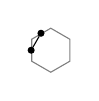
\begin{tikzpicture}[scale=1]
\node (h) [draw, color=gray, shape border rotate=30, minimum size=0.22in, regular polygon, regular polygon sides=6] at (0,0) {};
\node at (h.side 2) [draw,circle,fill,inner sep=0.75pt] (s1) {};
\node at (h.side 1) [draw,circle,fill,inner sep=0.75pt] (s2) {};
\draw (s1)--(s2);
\end{tikzpicture}
}

\newcommand{\transitiononefive}{
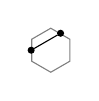
\begin{tikzpicture}[scale=1]
\node (h) [draw, color=gray, shape border rotate=30, minimum size=0.22in, regular polygon, regular polygon sides=6] at (0,0) {};
\node at (h.side 2) [draw,circle,fill,inner sep=0.75pt] (s1) {};
\node at (h.side 6) [draw,circle,fill,inner sep=0.75pt] (s2) {};
\draw (s1)--(s2);
\end{tikzpicture}
}

\newcommand{\transitiontwoone}{
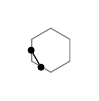
\begin{tikzpicture}[scale=1]
\node (h) [draw, color=gray, shape border rotate=30, minimum size=0.22in, regular polygon, regular polygon sides=6] at (0,0) {};
\node at (h.side 3) [draw,circle,fill,inner sep=0.75pt] (s1) {};
\node at (h.side 2) [draw,circle,fill,inner sep=0.75pt] (s2) {};
\draw (s1)--(s2);
\end{tikzpicture}
}

\newcommand{\transitiontwozero}{
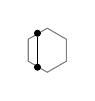
\begin{tikzpicture}[scale=1]
\node (h) [draw, color=gray, shape border rotate=30, minimum size=0.22in, regular polygon, regular polygon sides=6] at (0,0) {};
\node at (h.side 3) [draw,circle,fill,inner sep=0.75pt] (s1) {};
\node at (h.side 1) [draw,circle,fill,inner sep=0.75pt] (s2) {};
\draw (s1)--(s2);
\end{tikzpicture}
}

\newcommand{\transitiontwofive}{
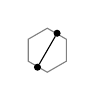
\begin{tikzpicture}[scale=1]
\node (h) [draw, color=gray, shape border rotate=30, minimum size=0.22in, regular polygon, regular polygon sides=6] at (0,0) {};
\node at (h.side 3) [draw,circle,fill,inner sep=0.75pt] (s1) {};
\node at (h.side 6) [draw,circle,fill,inner sep=0.75pt] (s2) {};
\draw (s1)--(s2);
\end{tikzpicture}
}

\newcommand{\transitiontwofour}{
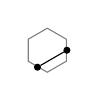
\begin{tikzpicture}[scale=1]
\node (h) [draw, color=gray, shape border rotate=30, minimum size=0.22in, regular polygon, regular polygon sides=6] at (0,0) {};
\node at (h.side 3) [draw,circle,fill,inner sep=0.75pt] (s1) {};
\node at (h.side 5) [draw,circle,fill,inner sep=0.75pt] (s2) {};
\draw (s1)--(s2);
\end{tikzpicture}
}

\newcommand{\transitionthreeone}{
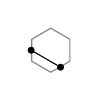
\begin{tikzpicture}[scale=1]
\node (h) [draw, color=gray, shape border rotate=30, minimum size=0.22in, regular polygon, regular polygon sides=6] at (0,0) {};
\node at (h.side 4) [draw,circle,fill,inner sep=0.75pt] (s1) {};
\node at (h.side 2) [draw,circle,fill,inner sep=0.75pt] (s2) {};
\draw (s1)--(s2);
\end{tikzpicture}
}

\newcommand{\transitionthreezero}{
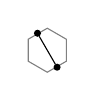
\begin{tikzpicture}[scale=1]
\node (h) [draw, color=gray, shape border rotate=30, minimum size=0.22in, regular polygon, regular polygon sides=6] at (0,0) {};
\node at (h.side 4) [draw,circle,fill,inner sep=0.75pt] (s1) {};
\node at (h.side 1) [draw,circle,fill,inner sep=0.75pt] (s2) {};
\draw (s1)--(s2);
\end{tikzpicture}
}

\newcommand{\transitionthreefive}{
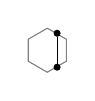
\begin{tikzpicture}[scale=1]
\node (h) [draw, color=gray, shape border rotate=30, minimum size=0.22in, regular polygon, regular polygon sides=6] at (0,0) {};
\node at (h.side 4) [draw,circle,fill,inner sep=0.75pt] (s1) {};
\node at (h.side 6) [draw,circle,fill,inner sep=0.75pt] (s2) {};
\draw (s1)--(s2);
\end{tikzpicture}
}

\newcommand{\transitionthreefour}{
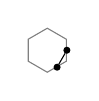
\begin{tikzpicture}[scale=1]
\node (h) [draw, color=gray, shape border rotate=30, minimum size=0.22in, regular polygon, regular polygon sides=6] at (0,0) {};
\node at (h.side 4) [draw,circle,fill,inner sep=0.75pt] (s1) {};
\node at (h.side 5) [draw,circle,fill,inner sep=0.75pt] (s2) {};
\draw (s1)--(s2);
\end{tikzpicture}
}

\newcommand{\transitionfourzero}{
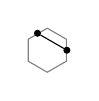
\begin{tikzpicture}[scale=1]
\node (h) [draw, color=gray, shape border rotate=30, minimum size=0.22in, regular polygon, regular polygon sides=6] at (0,0) {};
\node at (h.side 5) [draw,circle,fill,inner sep=0.75pt] (s1) {};
\node at (h.side 1) [draw,circle,fill,inner sep=0.75pt] (s2) {};
\draw (s1)--(s2);
\end{tikzpicture}
}

\newcommand{\transitionfourfive}{
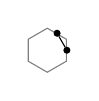
\begin{tikzpicture}[scale=1]
\node (h) [draw, color=gray, shape border rotate=30, minimum size=0.22in, regular polygon, regular polygon sides=6] at (0,0) {};
\node at (h.side 5) [draw,circle,fill,inner sep=0.75pt] (s1) {};
\node at (h.side 6) [draw,circle,fill,inner sep=0.75pt] (s2) {};
\draw (s1)--(s2);
\end{tikzpicture}
}


\newcommand{\growth}{
\begin{tikzpicture}[scale=1, transform shape]
\clip (1.3,-1) rectangle (6,2.8);

\node [draw, color=red!50, shape border rotate=30, minimum size=1.2in, regular polygon, regular polygon sides=6] at (2.93,1.18) (H1) {};

\node [draw,circle,fill,color=red!50,inner sep=0.5pt] at (2.93,1.18) (c1) {};

\node [draw, color=blue!50, shape border rotate=30, minimum size=1.2in, regular polygon, regular polygon sides=6] at (3.67,0.75) (H2) {};

\node [draw,circle,fill,color=blue!50,inner sep=0.5pt] at (3.67,0.75) (c2) {};


\node at (H2.side 6) [xshift=-0.3cm,yshift=0.18cm,draw,circle,fill,inner sep=1.4pt,label=0:{$u$}] (u) {};

\node at (H2.side 3) [xshift=-0.4cm,yshift=0.24cm,draw,circle,fill,inner sep=1.4pt,label=-180:{$l$}] (l) {};

\draw (u) -- (H2.corner 1) [->,>=stealth',blue];
\draw ($(u) + (-0.1cm,-0.052cm)$) -- ($(H1.corner 1) + (0,-0.1cm)$) [->,>=stealth',red];


\coordinate (c1r) at ($(c1)+(0:4)$);
\coordinate (c2u) at ($(c2)+(90:4)$);

\coordinate (z) at (intersection of c1--c1r and c2--c2u);

\draw [gray,<->,{Stealth-Stealth}] (c1) -- (z)  node [midway, above] {\scriptsize $\Delta x=1$};

\draw [densely dotted, gray] (c2) -- (z);

\coordinate (a) at (H1.corner 1);
\coordinate (b) at (H2.corner 1);

\draw [very thick,gray,<->,{Stealth-Stealth}] (a) -- (b)  node [midway, below left=-2pt] {\scriptsize $\Delta p_N(x)=\frac{2}{\sqrt{3}}$};

\coordinate (ar) at ($(a)+(0:4)$);
\coordinate (bu) at ($(b)+(90:4)$);

\coordinate (z) at (intersection of a--ar and b--bu);

\draw [gray,<->,{Stealth-Stealth}] (b) -- (z)  node [midway, right=-2pt] {\scriptsize $\Delta y(N(x)) = -\frac{1}{\sqrt{3}}$};


\coordinate (a) at (H1.side 2);
\coordinate (b) at (H2.side 2);

\coordinate (ar) at ($(a)+(0:4)$);
\coordinate (bu) at ($(b)+(90:4)$);

\coordinate (z) at (intersection of a--ar and b--bu);

\draw [gray,<->,{Stealth-Stealth}] (a) -- (z)  node [midway, below] {\scriptsize $\Delta w(x) = 1$};

\coordinate (a) at (H1.side 5);
\coordinate (b) at (H2.side 5);

\coordinate (ar) at ($(a)+(-90:4)$);
\coordinate (bu) at ($(b)+(180:4)$);

\coordinate (z) at (intersection of a--ar and b--bu);

\draw [gray,<->,{Stealth-Stealth}] (z) -- (b)  node [midway, below] {\scriptsize $\Delta e(x) = 1$};



\draw (l) -- (H2.corner 4) [->,>=stealth',blue];
\draw ($(l) + (0,-0.1cm)$) -- ($(H1.corner 4) + (0,-0.1cm)$) [->,>=stealth',red];

\coordinate (a) at (H1.corner 4);
\coordinate (b) at (H2.corner 4);

\draw [gray,<->,{Stealth-Stealth}] ($(H1.corner 4) + (0,-0.1cm)$) -- ($(H2.corner 4) + (0,-0.1cm)$)  node [midway, left=3pt] {\scriptsize $\Delta p_S(x)=\frac{2}{\sqrt{3}}$};

\coordinate (ar) at ($(a)+(0:4)$);
\coordinate (bu) at ($(b)+(90:4)$);

\coordinate (z) at (intersection of a--ar and b--bu);

\draw [gray,<->,{Stealth-Stealth}] ($(H2.corner 4) + (0,0.1cm)$) -- (z) node [midway, right=-2pt] {\scriptsize $\Delta y(S(x))=-\frac{3}{\sqrt{3}}$};
\end{tikzpicture}\hspace{-0.8cm}
\begin{tikzpicture}[scale=1, transform shape]
\clip (0.5,-1.55) rectangle (6.5,3.1);

\node [draw, color=red!50, shape border rotate=30, minimum size=1in, regular polygon, regular polygon sides=6] at (2.7,1.3) (H1) {};

\node [draw,circle,fill,color=red!50,inner sep=0.5pt] at (2.7,1.3) (c1) {};

\node [draw, color=blue!50, shape border rotate=30, minimum size=1.54in, regular polygon, regular polygon sides=6] at (3.3,0.965) (H2) {};

\node [draw,circle,fill,color=blue!50,inner sep=0.5pt] at (3.3,0.965) (c2) {};


\node at (H2.side 1) [xshift=-0.3cm,yshift=-0.18cm,draw,circle,fill,inner sep=1.4pt,label=180:{$u$}] (u) {};

\node at (H2.side 2) [draw,circle,fill,inner sep=1.4pt,label=-135:{$l$}] (l) {};

\draw (u) -- (H2.corner 1) [->,>=stealth',blue];
\draw ($(u) + (0.1cm,-0.052cm)$) -- ($(H1.corner 1) + (0,-0.1cm)$) [->,>=stealth',red];


\coordinate (c1r) at ($(c1)+(0:4)$);
\coordinate (c2u) at ($(c2)+(90:4)$);

\coordinate (z) at (intersection of c1--c1r and c2--c2u);

\draw [gray,<->,{Stealth-Stealth}] (c1) -- (z)  node [midway, above] {\scriptsize $\Delta x=1$};

\draw [densely dotted, gray] (c2) -- (z);

\coordinate (a) at (H1.corner 1);
\coordinate (b) at (H2.corner 1);

\draw [very thick,gray,<->,{Stealth-Stealth}] ($(a) + (0,-0.1cm)$) -- ($(b) + (0,-0.1cm)$)  node [midway, right=3pt] {\scriptsize $\Delta p_N(x)=\frac{2}{\sqrt{3}}$};

\coordinate (ar) at ($(a)+(90:4)$);
\coordinate (bu) at ($(b)+(180:4)$);

\coordinate (z) at (intersection of a--ar and b--bu);

\draw [gray,<->,{Stealth-Stealth}] (a) -- (z)  node [midway, left=-2pt] {\scriptsize $\Delta y(N(x)) = \frac{1}{\sqrt{3}}$};


%\coordinate (a) at (H1.side 2);
%\coordinate (b) at (H2.side 2);

%\coordinate (ar) at ($(a)+(0:4)$);
%\coordinate (bu) at ($(b)+(90:4)$);

%\coordinate (z) at (intersection of a--ar and b--bu);

\node at ($(H1.side 2) + (0.1cm,0)$) [gray] {\scriptsize $\Delta w(x) = 0$};
%\draw [gray,<->,{Stealth-Stealth}] (a) -- (z)  node [midway, above] {\scriptsize $\Delta w(x) = 0$};

\coordinate (a) at (H1.side 5);
\coordinate (b) at (H2.side 5);

\coordinate (ar) at ($(a)+(-90:4)$);
\coordinate (bu) at ($(b)+(180:4)$);

\coordinate (z) at (intersection of a--ar and b--bu);

\draw [gray,<->,{Stealth-Stealth}] (z) -- (b)  node [midway, below] {\scriptsize $\Delta e(x) = 2$};

\draw (l) -- (H2.corner 3) -- (H2.corner 4) [->,>=stealth',blue];
\draw ($(l) + (-0.052cm,0)$) -- ($(H1.corner 3) + (-0.052cm,-0.1cm)$) -- ($(H1.corner 4) + (0,-0.1cm)$) [->,>=stealth',red];

\coordinate (a) at (H1.corner 4);
\coordinate (b) at (H2.corner 4);

\coordinate (ad) at ($(a)+(-90:4)$);
\coordinate (bl) at ($(b)+(150:4)$);

\coordinate (z) at (intersection of a--ad and b--bl);

\draw [gray,<->,{Stealth-Stealth}] ($(H1.corner 4) + (0,-0.1cm)$) -- ($(z) + (0,0.1cm)$) -- ($(H2.corner 4) + (0,0.1cm)$)  node [yshift=0.3cm, midway, left=5pt] {\scriptsize $\Delta p_S(x)=\frac{4}{\sqrt{3}}$};

\coordinate (ar) at ($(a)+(0:4)$);
\coordinate (bu) at ($(b)+(90:4)$);

\coordinate (z) at (intersection of a--ar and b--bu);

\draw [gray,<->,{Stealth-Stealth}] ($(H2.corner 4) + (0,0.1cm)$) -- (z) node [midway, right=-3pt] {\scriptsize $\Delta y(S(x))=-\frac{3}{\sqrt{3}}$};
\end{tikzpicture}\hspace{-1cm}
\begin{tikzpicture}[scale=1, transform shape]
\clip (1.1,-2.25) rectangle (5.9,2.5);

\node [draw, color=blue!50, shape border rotate=30, minimum size=1.2in, regular polygon, regular polygon sides=6] at (3.94,-0.57) (H2) {};

\node [draw,circle,fill,color=blue!50,inner sep=0.5pt] at (3.94,-0.57) (c1) {};

\node [draw, color=red!50, shape border rotate=30, minimum size=1.66in, regular polygon, regular polygon sides=6] at (3.435,0.305) (H1) {};

\node [draw,circle,fill,color=red!50,inner sep=0.5pt] at (3.435,0.305) (c2) {};


\node at (H1.side 5) [yshift=-0.4cm,draw,circle,fill,inner sep=1.4pt,label=0:{$u$}] (u) {};

\node at (H1.side 3) [xshift=0.5cm,yshift=-0.29cm,draw,circle,fill,inner sep=1.4pt,label=180:{$l$}] (l) {};

\draw ($(u) + (0.052cm,0cm)$) -- ($(H1.corner 6) + (0.052cm,0.1cm)$) -- ($(H1.corner 1) + (0,0.1cm)$) [->,>=stealth',red];
\draw (u) -- (H2.corner 6) -- (H2.corner 1) [->,>=stealth',blue];


\coordinate (c1r) at ($(c1)+(0:4)$);
\coordinate (c2u) at ($(c2)+(90:4)$);

\coordinate (z) at (intersection of c1--c1r and c2--c2u);

\draw [gray,<->,{Stealth-Stealth}] (c1) -- (z)  node [midway, above] {\scriptsize $\Delta x=1$};

\draw [densely dotted, gray] (c2) -- (z);

\coordinate (a) at (H1.corner 1);
\coordinate (b) at (H2.corner 1);


\coordinate (ar) at ($(a)+(-30:4)$);
\coordinate (bu) at ($(b)+(90:4)$);

\coordinate (z) at (intersection of a--ar and b--bu);

\draw [very thick,gray,<->,{Stealth-Stealth}] (a) -- (z) -- (b)  node [near end, right=0pt] {\scriptsize $\Delta p_N(x)=\frac{6}{\sqrt{3}}$};

\coordinate (ad) at ($(a)+(-90:4)$);
\coordinate (bl) at ($(b)+(180:4)$);

\coordinate (z) at (intersection of a--ad and b--bl);

\draw [gray,<->,{Stealth-Stealth}] (a) -- (z)  node [midway, left=-1pt] {\scriptsize $\Delta y(N(x)) = -\frac{1}{\sqrt{3}}$};


\node at (H2.side 5) [gray] {\scriptsize $\Delta e(x) = 0$};

\coordinate (a) at ($(H1.side 2) + (0,-0.2cm)$);
\coordinate (b) at (H2.side 2);

\coordinate (ar) at ($(a)+(0:4)$);
\coordinate (bu) at ($(b)+(90:4)$);

\coordinate (z) at (intersection of a--ar and b--bu);

\draw [gray,<->,{Stealth-Stealth}] (z) -- (a)  node [midway, above] {\scriptsize $\Delta w(x) = 2$};

\draw (l) -- (H2.corner 4) [->,>=stealth',blue];

\draw ($(l) + (0,-0.1cm)$) -- ($(H1.corner 4) + (0,-0.1cm)$) [->,>=stealth',red];

\coordinate (a) at (H1.corner 4);
\coordinate (b) at (H2.corner 4);

\draw [gray,<->,{Stealth-Stealth}] ($(H1.corner 4) + (0,-0.1cm)$) -- ($(H2.corner 4) + (0,-0.1cm)$)  node [midway, above right=-3pt] {\scriptsize $\Delta p_S(x)=\frac{2}{\sqrt{3}}$};

\coordinate (ad) at ($(a)+(-90:4)$);
\coordinate (bl) at ($(b)+(180:4)$);

\coordinate (z) at (intersection of a--ad and b--bl);

\draw [gray,<->,{Stealth-Stealth}] ($(H1.corner 4) + (0,-0.1cm)$) -- ($(z) + (0,-0.1cm)$) node [midway, left=0pt] {\scriptsize $\Delta y(S(x))=-\frac{3}{\sqrt{3}}$};


\end{tikzpicture}
%\begin{tikzpicture}[scale=1, transform shape]
%\clip (1,-2) rectangle (5.7,2.8);

%\node [draw, color=red!50, shape border rotate=30, minimum size=1.2in, regular polygon, regular polygon sides=6] at (2.93,1.18) (H1) {};

%\node [draw,circle,fill,color=red!50,inner sep=0.5pt] at (2.93,1.18) (c1) {};

%\node [draw, color=blue!50, shape border rotate=30, minimum size=1.66in, regular polygon, regular polygon sides=6] at (3.435,0.305) (H2) {};

%\node [draw,circle,fill,color=blue!50,inner sep=0.5pt] at (3.435,0.305) (c2) {};


%\node at (H2.side 6) [xshift=-0.5cm,yshift=0.29cm,draw,circle,fill,inner sep=1.4pt,label=0:{$u$}] (u) {};

%\node at (H2.side 2) [yshift=0.4cm,draw,circle,fill,inner sep=1.4pt,label=-135:{$l$}] (l) {};

%\draw (u) -- (H2.corner 1) [->,>=stealth',blue];
%\draw ($(u) + (-0.1cm,-0.052cm)$) -- ($(H1.corner 1) + (0,-0.1cm)$) [->,>=stealth',red];


%\coordinate (c1r) at ($(c1)+(0:4)$);
%\coordinate (c2u) at ($(c2)+(90:4)$);

%\coordinate (z) at (intersection of c1--c1r and c2--c2u);

%\draw [gray,<->,{Stealth-Stealth}] (c1) -- (z)  node [midway, above] {\scriptsize $\Delta(x)=1$};

%\draw [densely dotted, gray] (c2) -- (z);

%\coordinate (a) at (H1.corner 1);
%\coordinate (b) at (H2.corner 1);

%\draw [very thick,gray,<->,{Stealth-Stealth}] (a) -- (b)  node [midway, below left=-2pt] {\scriptsize $\Delta p_N(x)=\frac{2}{\sqrt{3}}$};

%\coordinate (ar) at ($(a)+(0:4)$);
%\coordinate (bu) at ($(b)+(90:4)$);

%\coordinate (z) at (intersection of a--ar and b--bu);

%\draw [gray,<->,{Stealth-Stealth}] (b) -- (z)  node [midway, right=-2pt] {\scriptsize $\Delta y(N(x)) = -\frac{1}{\sqrt{3}}$};


%\node at ($(H1.side 2) + (0.2cm,0)$) [gray] {\scriptsize $\Delta w(x) = 0$};

%\coordinate (a) at (H1.side 5);
%\coordinate (b) at (H2.side 5);

%\coordinate (ar) at ($(a)+(0:4)$);
%\coordinate (bu) at ($(b)+(90:4)$);

%\coordinate (z) at (intersection of a--ar and b--bu);

%\draw [gray,<->,{Stealth-Stealth}] (z) -- (a)  node [midway, below] {\scriptsize $\Delta e(x) = 2$};

%\draw (l) -- (H2.corner 3) -- (H2.corner 4) [->,>=stealth',blue];
%\draw ($(l) + (-0.052cm,0)$) -- ($(H1.corner 3) + (-0.052cm,-0.1cm)$) -- ($(H1.corner 4) + (0,-0.1cm)$) [->,>=stealth',red];

%\coordinate (a) at (H1.corner 4);
%\coordinate (b) at (H2.corner 4);

%\coordinate (ad) at ($(a)+(-90:4)$);
%\coordinate (bl) at ($(b)+(150:4)$);

%\coordinate (z) at (intersection of a--ad and b--bl);

%\draw [gray,<->,{Stealth-Stealth}] ($(H1.corner 4) + (0,-0.1cm)$) -- ($(z) + (0,0.1cm)$) -- ($(H2.corner 4) + (0,0.1cm)$)  node [midway, left=6pt] {\scriptsize $\Delta p_S(x)=\frac{6}{\sqrt{3}}$};

%\coordinate (ar) at ($(a)+(0:4)$);
%\coordinate (bu) at ($(b)+(90:4)$);

%\coordinate (z) at (intersection of a--ar and b--bu);

%\draw [gray,<->,{Stealth-Stealth}] ($(H2.corner 4) + (0,0.1cm)$) -- (z) node [midway, right=-2pt] {\scriptsize $\Delta y(S(x))=-\frac{5}{\sqrt{3}}$};
%\end{tikzpicture}
}





\newcommand{\badintervals}{
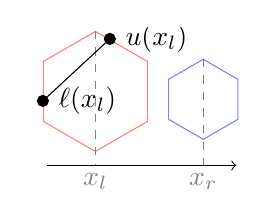
\begin{tikzpicture}[scale=1, transform shape]
\clip (.6,-.67) rectangle (3.3,1.4);

\node [draw, color=red!50, shape border rotate=30, minimum size=0.6in, regular polygon, regular polygon sides=6] at (1.46,0.59) (H1) {};

\coordinate (c1) at (1.46,0.59);

\node [draw, color=blue!50, shape border rotate=30, minimum size=0.4in, regular polygon, regular polygon sides=6] at (2.83,0.49) (H2) {};

\coordinate (c2) at (2.83,0.49);

\node at (H1.side 6) [xshift=-0.15cm,yshift=0.09cm,draw,circle,fill,inner sep=1.4pt,label=0:{$u(x_l)$}] (ul) {};

\node at (H1.side 2) [yshift=-0.12cm,draw,circle,fill,inner sep=1.4pt,label=0:{$\ell(x_l)$}] (l) {};

\draw [->] (0.85,-0.35) -- (3.25,-0.35);

\coordinate (N1) at (H1.corner 1);
\coordinate (N2) at (H2.corner 1);

\draw [gray, dashed] (N1) -- (1.46,-0.35);
\draw [gray, dashed] (N2) -- (2.83,-0.35);

\node at (1.46,-0.35) [label={[label distance=-0.15cm]-90:{\color{gray}{$x_l$}}}] {};
\node at (2.83,-0.35) [label={[label distance=-0.15cm]-90:{\color{gray}{$x_r$}}}] {};

\draw (ul) -- (l);

\end{tikzpicture}\hspace{0.75cm}
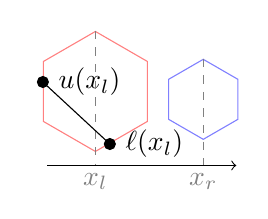
\begin{tikzpicture}[scale=1, transform shape]
\clip (.6,-.67) rectangle (3.3,1.4);

\node [draw, color=red!50, shape border rotate=30, minimum size=0.6in, regular polygon, regular polygon sides=6] at (1.46,0.59) (H1) {};

\coordinate (c1) at (1.46,0.59);

\node [draw, color=blue!50, shape border rotate=30, minimum size=0.4in, regular polygon, regular polygon sides=6] at (2.83,0.49) (H2) {};

\coordinate (c2) at (2.83,0.49);

\node at (H1.side 2) [yshift=0.12cm,draw,circle,fill,inner sep=1.4pt,label=0:{$u(x_l)$}] (ul) {};

\node at (H1.side 4) [xshift=-0.15cm,yshift=-0.09cm,draw,circle,fill,inner sep=1.4pt,label=0:{$\ell(x_l)$}] (l) {};

\draw [->] (0.85,-0.35) -- (3.25,-0.35);

\coordinate (N1) at (H1.corner 1);
\coordinate (N2) at (H2.corner 1);

\draw [gray, dashed] (N1) -- (1.46,-0.35);
\draw [gray, dashed] (N2) -- (2.83,-0.35);

\node at (1.46,-0.35) [label={[label distance=-0.15cm]-90:{\color{gray}{$x_l$}}}] {};
\node at (2.83,-0.35) [label={[label distance=-0.15cm]-90:{\color{gray}{$x_r$}}}] {};

\draw (ul) -- (l);

\end{tikzpicture}\hspace{0.75cm}
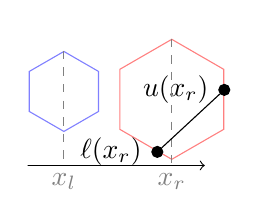
\begin{tikzpicture}[scale=1, transform shape]
\clip (1,-.67) rectangle (3.6,1.4);

\node [draw, color=red!50, shape border rotate=30, minimum size=0.6in, regular polygon, regular polygon sides=6] at (2.83,0.49) (H2) {};

\coordinate (c1) at (1.46,0.59);

\node [draw, color=blue!50, shape border rotate=30, minimum size=0.4in, regular polygon, regular polygon sides=6] at (1.46,0.59) (H1) {};

\coordinate (c2) at (2.83,0.49);

\node at (H2.side 5) [yshift=0.12cm,draw,circle,fill,inner sep=1.4pt,label=180:{$u(x_r)$}] (ul) {};

\node at (H2.side 3) [yshift=-0.09cm,xshift=0.15cm,draw,circle,fill,inner sep=1.4pt,label=180:{$\ell(x_r)$}] (l) {};

\draw [->] (0.85,-0.35) -- (3.25,-0.35);

\coordinate (N1) at (H1.corner 1);
\coordinate (N2) at (H2.corner 1);

\draw [gray, dashed] (N1) -- (1.46,-0.35);
\draw [gray, dashed] (N2) -- (2.83,-0.35);

\node at (1.46,-0.35) [label={[label distance=-0.15cm]-90:{\color{gray}{$x_l$}}}] {};
\node at (2.83,-0.35) [label={[label distance=-0.15cm]-90:{\color{gray}{$x_r$}}}] {};

\draw (ul) -- (l);

\end{tikzpicture}\hspace{0.75cm}
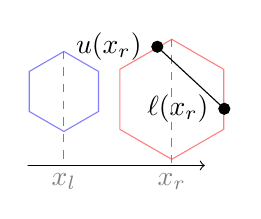
\begin{tikzpicture}[scale=1, transform shape]
\clip (1,-.67) rectangle (3.6,1.4);

\node [draw, color=red!50, shape border rotate=30, minimum size=0.6in, regular polygon, regular polygon sides=6] at (2.83,0.49) (H2) {};

\coordinate (c1) at (1.46,0.59);

\node [draw, color=blue!50, shape border rotate=30, minimum size=0.4in, regular polygon, regular polygon sides=6] at (1.46,0.59) (H1) {};

\coordinate (c2) at (2.83,0.49);

\node at (H2.side 1) [xshift=0.15cm,yshift=0.09cm,draw,circle,fill,inner sep=1.4pt,label=180:{$u(x_r)$}] (ul) {};

\node at (H2.side 5) [yshift=-0.12cm,draw,circle,fill,inner sep=1.4pt,label=180:{$\ell(x_r)$}] (l) {};

\draw [->] (0.85,-0.35) -- (3.25,-0.35);

\coordinate (N1) at (H1.corner 1);
\coordinate (N2) at (H2.corner 1);

\draw [gray, dashed] (N1) -- (1.46,-0.35);
\draw [gray, dashed] (N2) -- (2.83,-0.35);

\node at (1.46,-0.35) [label={[label distance=-0.15cm]-90:{\color{gray}{$x_l$}}}] {};
\node at (2.83,-0.35) [label={[label distance=-0.15cm]-90:{\color{gray}{$x_r$}}}] {};

\draw (ul) -- (l);

\end{tikzpicture}
}








\newcommand{\gentlepath}{
\begin{tikzpicture}[scale=1, transform shape]
%\clip (1.3,-1) rectangle (8,2.8);

\node [draw, color=red!50, shape border rotate=30, minimum size=1.2in, regular polygon, regular polygon sides=6] at (2.93,1.18) (H1) {};

\coordinate (c1) at (2.93,1.18);

\node at (H1.side 6) [xshift=-0.3cm,yshift=0.18cm,draw,circle,fill,inner sep=1.4pt,label={[label distance=0pt]0:$u(x)$}] (ul) {};

\node at ($(ul)+(0,-0.85)$) [inner sep=0pt,outer sep=-0.2pt] (x) {};
\draw [gray,<->,{Stealth-Stealth}] (x) -- ($(x)+(0.95,0)$) node [below left] {\scriptsize $\delta_f(x)$};

\draw [gray,dashed] (ul) -- (ul |- 1, 1.65);

\node at (H1.side 2) [yshift=-0.24cm,draw,circle,fill,inner sep=1.4pt,label={[label distance=-3pt]135:$\ell(x)$}] (l) {};

\draw [thick] (ul) -- (l);

\node at (H1.corner 3) [draw,gray,circle,fill,inner sep=0.5pt,label=-180:{$w$}] (w) {};

\draw [->] (1,0.1) -- (4.5,0.1);

\coordinate (N1) at (H1.corner 1);

\node at (N1) [label={[label distance=-0.3cm]135:{\scriptsize $N(x)$}}] {};

\draw [gray] (ul) -- (w) -- (N1);

\draw [gray, dashed] (N1) -- (2.93,0.1);

\draw pic [draw=gray, "\color{gray}{\scriptsize $\theta$}", angle eccentricity=1.25,angle radius=1.05cm] {angle = ul--w--N1};


\node at (2.93,0.1) [label={[label distance=-0.15cm]-90:{\color{gray}{$x$}}}] {};

\draw [gray,<->,{Stealth-Stealth},label=90:${\tt r}(x)$] ($(w)+(2.64,0.2)$$) -- ($(w)+(1.32,0.2)$) node [midway, above] {\scriptsize ${\tt r}(x)$};

\draw (l) -- (H1.corner 3) -- (H1.corner 4) [->,>=stealth',blue,thick];
\draw (ul) -- (H1.corner 1) [->,>=stealth',red,thick];
%\draw ($(l) + (-0.052cm,0)$) -- ($(H1.corner 3) + (-0.052cm,-0.1cm)$) -- ($(H1.corner 4) + (0,-0.1cm)$) [->,>=stealth',red];

\node at (H1.side 6) [red,xshift=0.75,yshift=0.6cm] {$p_N(x) (-)$};

\node at (H1.side 3) [blue,xshift=-0.8cm,yshift=-0.2cm] {$p_S(x) (+)$};


\end{tikzpicture}\hspace{1cm}
\begin{tikzpicture}[scale=1, transform shape]
%\clip (1.3,-1) rectangle (8,2.8);

\node [draw, color=red!50, shape border rotate=30, minimum size=1.2in, regular polygon, regular polygon sides=6] at (2.93,1.18) (H1) {};

\coordinate (c1) at (2.93,1.18);

\node [draw, color=blue!50, shape border rotate=30, minimum size=0.8in, regular polygon, regular polygon sides=6] at (5.67,0.99) (H2) {};

\coordinate (c2) at (5.67,0.99);

\node at (H1.side 6) [xshift=-0.3cm,yshift=0.18cm,draw,circle,fill,inner sep=1.4pt,label=45:{$u(x_l)=u_i$}] (ul) {};

\node at (H1.side 2) [yshift=-0.24cm,draw,circle,fill,inner sep=1.4pt,label={[label distance=-3pt]135:$l_i = \ell(x_l)$}] (l) {};



%\node at (H1.side 6) [xshift=-0.3cm,yshift=0.18cm,draw,circle,fill,inner sep=1.4pt,label=45:{$u(x_l)$}] (ul) {};

%\draw [gray,<->,{Stealth-Stealth},label=90:$\theta_f(x_l)$] ($(ul)+(0,-1.3)$) -- ($(ul)+(-0.36,-1.3)$) node [above right] {\scriptsize ${\tt r}(x_l)-\delta_f(x_l)$};

\draw [gray,<->,{Stealth-Stealth}] ($(ul)+(0,-1.5)$) -- ($(ul)+(0.95,-1.5)$) node [midway, below] {\scriptsize $\delta_f(x_l)$};

%\node at (H1.side 2) [yshift=-0.24cm,draw,circle,fill,inner sep=1.4pt,label=135:{$\ell(x_l)$}] (l) {};

%\node at (H2.side 6) [xshift=+0.3cm,yshift=-0.18cm,draw,circle,fill,inner sep=1.4pt,label=45:{$u_{i+s}=u(x_r)$}] (ur) {};

\node at (H1.corner 3) (w) {};

\draw [->] (1,0.1) -- (7,0.1);

\coordinate (N1) at (H1.corner 1);
\coordinate (N2) at (H2.corner 1);

%\draw (N1) -- ++(-30:0.65) -- ++(30:0.35) -- ++(-90:.25) -- ++ (-30:1.1) -- ++ (30:0.6);


\coordinate (N12) at ($(ul)+(30:0.25)$);
\coordinate (N13) at ($(N12)+(-30:0.5)$);
\coordinate (N14) at ($(N13)+(-90:.35)$);
\coordinate (N15) at ($(N14)+(-30:0.8)$);



%\draw [decorate,decoration={brace,amplitude=10pt},xshift=-4pt,yshift=0pt]
%(0.5,0.5) -- (0.5,5.0) node [black,midway,xshift=-0.6cm] 
%{\footnotesize $P_1$};

\coordinate (x) at ($(N15)+(30:.66)$);

\coordinate (xd) at ($(x)+(30:6)$);
\coordinate (N2d) at ($(N2)+(150:4)$);

\coordinate (z) at (intersection of N2--N2d and x--xd);

\draw [densely dotted,thick] (N1) -- (ul) -- (N12) -- (N13) -- (N14) -- (N15) -- (x) -- (z) -- (N2);



\coordinate (N1d) at ($(N1)+(-90:3)$);
\coordinate (ud) at ($(ul)+(-90:3)$);
\coordinate (N12d) at ($(N12)+(-90:3)$);
\coordinate (N15d) at ($(N15)+(-90:3)$);
\coordinate (zd) at ($(z)+(-90:3)$);
\coordinate (N2d) at ($(N2)+(-90:3)$);


\coordinate (N1b) at ($(N1)+(0,-0.9)$);
\coordinate (N1r) at ($(N1b)+(0:10)$);

\coordinate (z1) at (intersection of N1--N1d and N1b--N1r);
\coordinate (z2) at (intersection of ul--ud and N1b--N1r);
\coordinate (z3) at (intersection of N12--N12d and N1b--N1r);
\coordinate (z4) at (intersection of N15--N15d and N1b--N1r);
\coordinate (z5) at (intersection of z--zd and N1b--N1r);
\coordinate (z6) at (intersection of N2--N2d and N1b--N1r);

\draw [gray!50, densely dashed] (ul) -- ($(ul)+(0,-1.5)$);
\draw [gray!50, densely dashed] (N12) -- (z3);
\draw [gray!50, densely dashed] (z) -- (z5);
\draw [gray!50, densely dashed] (z4) -- (N15);


\draw [blue, very thick] (z1) -- (z2);
\draw [blue, very thick] (z3) -- (z4);
\draw [blue, very thick] (z5) -- (z6);





\node at (N1) [label={[label distance=-0.3cm]135:{\scriptsize $N(x_l)$}}] {};
\node at (N2) [label={[label distance=-0.3cm]45:{\scriptsize $N(x_r)$}}] {};

%\draw [gray] (ul) -- (w) -- (N1);

\draw [gray, dashed] (N1) -- (2.93,0.1);
\draw [gray, dashed] (N2) -- (5.67,0.1);

%\draw pic [draw=gray, "\color{gray}{\scriptsize $\Theta$}", angle eccentricity=1.25,angle radius=1.05cm] {angle = ul--w--N1};


\node at (2.93,0.1) [label={[label distance=-0.15cm]-90:{\color{gray}{$x_l$}}}] {};
\node at (5.67,0.1) [label={[label distance=-0.15cm]-90:{\color{gray}{$x_r$}}}] {};

\draw [gray,<->,{Stealth-Stealth},label=90:${\tt r}(x_l)$] ($(w)$) -- ($(w)+(1.32,0)$) node [midway, above] {\scriptsize ${\tt r}(x_l)$};


%\coordinate (lr) at ($(l)+(0:6)$);
%\coordinate (urd) at ($(ur)+(-90:4)$);

%\coordinate (z) at (intersection of l--lr and ur--urd);

%\draw [gray,<->,{Stealth-Stealth}] (ur) -- (z)  node [midway, right=2pt] {\scriptsize $y(u(x_r)) - y((x_l))$};

\draw (ul) -- (l);



\node at (H2.side 6) [xshift=+0.3cm,yshift=-0.18cm,draw,circle,fill,inner sep=1.4pt,label={[label distance=0pt]30:$u_{i+s} = u(x_r)$}] (ur) {};

\draw [densely dotted,thick] (N2) -- (ur);




\coordinate (lr) at ($(l)+(0:6)$);
\coordinate (urd) at ($(ur)+(-90:4)$);

\coordinate (z) at (intersection of l--lr and ur--urd);

\draw [gray,<->,{Stealth-Stealth}] (ur) -- (z)  node [midway, right=2pt] {\scriptsize $y(u(x_r)) - y(\ell(x_l))$};

\draw (ul) -- (l);

\end{tikzpicture}
}

\newcommand{\linearworstcase}{
\begin{tikzpicture}[scale=1, transform shape]
%\clip (1.3,-1) rectangle (8,2.8);

\node [draw, color=red!50, shape border rotate=30, minimum size=1.2in, regular polygon, regular polygon sides=6] at (2.93,1.18) (H1) {};

\coordinate (c1) at (2.93,1.18);

\node [draw, color=blue!50, shape border rotate=30, minimum size=0.8in, regular polygon, regular polygon sides=6] at (5.67,0.99) (H2) {};

\coordinate (c2) at (5.67,0.99);



\node at (H1.side 6) [xshift=-0.3cm,yshift=0.18cm,draw,circle,fill,inner sep=1.4pt,label=0:{$u(x_l)$}] (ul) {};

\draw [gray,<->,{Stealth-Stealth},label=90:$\theta_f(x_l)$] ($(ul)+(0,-1.1)$) -- ($(ul)+(0.96,-1.1)$) node [below left] {\scriptsize $\delta_f(x_l)$};

\draw [gray,<->,{Stealth-Stealth},label=90:$\theta_f(x_l)$] ($(ul)+(-0.96,-1.1)$) -- ($(ul)+(0,-1.1)$) node [below left] {\scriptsize $\delta_f(x_l)$};

\draw [gray, dashed] (ul) -- ($(ul)+(0,-1.1)$);


\node at (H1.side 2) [yshift=-0.24cm,draw,circle,fill,inner sep=1.4pt,label=180:{$\ell(x_l)$}] (l) {};

\draw [gray,<->,{Stealth-Stealth},label=90:$\theta_f(x_l)$] ($(l)+(0,-0.5)$) -- ($(l)+(0.36,-0.5)$) node [very near start, below] {\scriptsize ${\tt r}(x_l) - \delta_f(x_l)$};

% \draw [gray,<->,{Stealth-Stealth},label=90:$\theta_f(x_l)$] ($(l)+(0.36,-0.5)$) -- ($(l)+(0.72,-0.5)$) node [very near end, above] {\scriptsize $\theta_f(x)$};

%\draw [gray, dashed] ($(l)+(0.36,-0.1)$) -- ($(l)+(0.36,-0.5)$);

\node at (H2.side 5) [yshift=+0.18cm,draw,circle,fill,inner sep=1.4pt,label=45:{$u(x_r)$}] (ur) {};


%%%%%%%%%%%%%%%%%%%%%

\coordinate (N12) at ($(ul)+(30:0.25)$);

%\coordinate (N12d) at ($(N12)+(-90:3)$);
%\draw [gray, densely dashed] (N12) -- (N12d);

\coordinate (N13) at ($(N12)+(-30:0.35)$);
\coordinate (N14) at ($(N13)+(-90:.35)$);
\coordinate (N15) at ($(N14)+(-30:0.8)$);

%\coordinate (N15d) at ($(N15)+(-90:3)$);
%\draw [gray!50, densely dashed] (N15) -- (N15d);

\coordinate (x) at ($(N15)+(30:.66)$);

\coordinate (xd) at ($(x)+(30:6)$);
\coordinate (N2d) at ($(N2)+(150:4)$);

\coordinate (z) at (intersection of N2--N2d and x--xd);

\draw [densely dotted] (N1) -- (ul) -- (N12) -- (N13) -- (N14) -- (N15) -- (x) -- (z) -- (N2);





%\draw (ul) -- ++(-30:1) -- ++(30:0.5) -- ++(-30:.5) -- ++ (30:0.37) -- ++ (ur);

\draw [->] (1,0.1) -- (7,0.1);

\coordinate (N1) at (H1.corner 1);
\coordinate (N2) at (H2.corner 1);

%\node at (N1) [label={[label distance=-0.3cm]135:{\scriptsize $N(x_l)$}}] {};
%\node at (N2) [label={[label distance=-0.3cm]45:{\scriptsize $N(x_r)$}}] {};

%\draw [gray] (ul) -- (w) -- (N1);

\draw [gray, dashed] (N1) -- (2.93,0.1);
\draw [gray, dashed] (N2) -- (5.67,0.1);

%\draw pic [draw=gray, "\color{gray}{\scriptsize $\Theta$}", angle eccentricity=1.25,angle radius=1.05cm] {angle = ul--w--N1};


\node at (2.93,0.1) [label={[label distance=-0.15cm]-90:{\color{gray}{$x_l$}}}] {};
\node at (5.67,0.1) [label={[label distance=-0.15cm]-90:{\color{gray}{$x_r$}}}] {};

%\draw [blue,thick,<->,{Stealth-Stealth}] ($($(l)+(0.72,-0.1)$)$) -- ($($(l)+(2.36,0)$)+(2.59,-0.1)$) node [midway, above] {};

%\draw [red,thick,<->,{Stealth-Stealth},label=90:${\tt r}(x_l)$] ($($(l)+(0.36,-0.5)$)$) -- ($($(l)+(2.36,-0.5)$)+(1.7,0)$) node [midway, above] {};


\draw [blue,thick,<->,{Stealth-Stealth}] ($($(l)+(0.72,0)$)$) -- ($($(l)+(2.36,0.5)$)+(2.59,-0.5)$) node [midway, above] {};

\draw [red,thick,<->,{Stealth-Stealth},label=90:${\tt r}(x_l)$] ($($(l)+(0.36,-0.5)$)$) -- ($($(l)+(2.36,-0.5)$)+(1.7,0)$) node [midway, above] {};


%\coordinate (lr) at ($(l)+(0:6)$);
%\coordinate (urd) at ($(ur)+(-90:4)$);

%\coordinate (z) at (intersection of l--lr and ur--urd);

%\draw [gray,<->,{Stealth-Stealth}] (ur) -- (z)  node [midway, right=2pt] {\scriptsize $y(u(x_r)) - y((x_l))$};

\draw (ul) -- (l);
\end{tikzpicture}
\begin{tikzpicture}[scale=1, transform shape]
%\clip (1.3,-1) rectangle (8,2.8);

\node [draw, color=red!50, shape border rotate=30, minimum size=1.2in, regular polygon, regular polygon sides=6] at (2.93,1.18) (H1) {};

\coordinate (c1) at (2.93,1.18);

\node [draw, color=blue!50, shape border rotate=30, minimum size=0.8in, regular polygon, regular polygon sides=6] at (5.67,0.99) (H2) {};

\coordinate (c2) at (5.67,0.99);



\node at (H1.side 6) [xshift=-0.3cm,yshift=0.18cm,draw,circle,fill,inner sep=1.4pt,label=0:{$u(x_l)$}] (ul) {};

%\draw [gray,<->,{Stealth-Stealth},label=90:$\theta_f(x_l)$] ($(ul)+(0,-0.5)$) -- ($(ul)+(-0.36,-0.5)$) node [very near start, below] {\scriptsize $\theta_f(x_l)$};

\draw [gray,<->,{Stealth-Stealth},label=90:$\theta_f(x_l)$] ($(ul)+(0,-1.65)$) -- ($(ul)+(0.96,-1.65)$) node [below left] {\scriptsize $\delta_f(x_l)$};
\draw [gray,<->,{Stealth-Stealth},label=90:$\theta_f(x_l)$] ($(ul)+(-0.96,-1.65)$) -- ($(ul)+(0,-1.65)$) node [below left] {\scriptsize $\delta_f(x_l)$};


\draw [gray, dashed] (ul) -- ($(ul)+(0,-1.65)$);



\node at (H1.side 2) [yshift=-0.24cm,draw,circle,fill,inner sep=1.4pt,label=180:{$\ell(x_l)$}] (l) {};

%\draw [gray,<->,{Stealth-Stealth},label=90:$\theta_f(x_l)$] ($(l)+(0.36,-0.5)$) -- ($(l)+(0,-0.5)$) node [above right] {\scriptsize ${\tt r}(x_l) - \delta_f(x_l)$};

\node at (H2.corner 2) [draw,circle,fill,inner sep=1.4pt,label=0:{$u(x_r)$}] (ur) {};


%%%%%%%

\coordinate (N12) at ($(N1)+(-30:0.1)$);

%\coordinate (N12d) at ($(N12)+(-90:3)$);
%\draw [gray, densely dashed] (N12) -- (N12d);

\coordinate (N13) at ($(N12)+(-90:1)$);
%\coordinate (N14) at ($(N13)+(-30:1.85)$);
%\coordinate (N15) at ($(N14)+(-30:1.85)$);

%\coordinate (N15d) at ($(N15)+(-90:3)$);
%\draw [gray!50, densely dashed] (N15) -- (N15d);

%\coordinate (x) at ($(N13)+(-30:1.66)$);

\coordinate (xd) at ($(N13)+(-30:6)$);
\coordinate (N2d) at ($(N2)+(-150:4)$);

\coordinate (z) at (intersection of N2--N2d and N13--xd);

\draw [densely dotted] (N1) -- (N12) -- (N13) -- (z) -- (N2);

\coordinate (zd) at ($(z)+(0,-5)$);
\coordinate (N2d) at ($(N2)+(6,0)$);

\coordinate (zzz) at (intersection of zd--z and N2--N2d);

\draw [red,dashed,thick,<->,{Stealth-Stealth}] (N2) -- (zzz);

\draw [gray, dashed] (z) -- (zzz);





%\draw (ul) -- ++(-30:1) -- ++(30:0.5) -- ++(-30:.5) -- ++ (30:0.37) -- ++ (ur);

\draw [->] (1,0.1) -- (7,0.1);

\coordinate (N1) at (H1.corner 1);
\coordinate (N2) at (H2.corner 1);

%\node at (N1) [label={[label distance=-0.3cm]135:{\scriptsize $N(x_l)$}}] {};
%\node at (N2) [label={[label distance=-0.3cm]45:{\scriptsize $N(x_r)$}}] {};

%\draw [gray] (ul) -- (w) -- (N1);

\draw [gray, dashed] (N1) -- (2.93,0.1);

\draw [gray, dashed] (N2) -- (5.67,0.1);

%\draw pic [draw=gray, "\color{gray}{\scriptsize $\Theta$}", angle eccentricity=1.25,angle radius=1.05cm] {angle = ul--w--N1};


\node at (2.93,0.1) [label={[label distance=-0.15cm]-90:{\color{gray}{$x_l$}}}] {};
\node at (5.67,0.1) [label={[label distance=-0.15cm]-90:{\color{gray}{$x_r$}}}] {};

\draw [blue,thick,<->,{Stealth-Stealth}] ($($(l)+(0.72,-0.5)$)$) -- ($($(l)+(1.47,-0.5)$)+(1.7,0)$) node [midway, above] {};


%\coordinate (lr) at ($(l)+(0:6)$);
%\coordinate (urd) at ($(ur)+(-90:4)$);

%\coordinate (z) at (intersection of l--lr and ur--urd);

%\draw [gray,<->,{Stealth-Stealth}] (ur) -- (z)  node [midway, right=2pt] {\scriptsize $y(u(x_r)) - y((x_l))$};

\draw (ul) -- (l);
\end{tikzpicture} 
\vspace{-0.5cm}\center{(a) \hspace{2.6in} (b)}
}





\newcommand{\induction}{
\begin{tikzpicture}[scale=1, transform shape]
%\clip (1.3,-1) rectangle (8,2.8);

\node at (0,0.5) [draw,circle,fill,inner sep=1.4pt,label=180:{$p$}] (p) {};
\coordinate (pu) at ($(p)+(0,1)$);

\draw [gray, dashed] (p) -- (pu);

\coordinate (c1) at (2.93,1.18);

\node [draw, color=red!50, shape border rotate=30, minimum size=1.2in, regular polygon, regular polygon sides=6] at (c1) (H1) {};

\node at (H1.side 6) [xshift=-0.3cm,yshift=0.18cm,draw,circle,fill,inner sep=1.4pt,label=0:{$u(x)$}] (ul) {};

\draw [gray,<->,{Stealth-Stealth}] ($(ul)+(0,-0.7)$) -- ($(ul)+(0.96,-0.7)$) node [below left] {\scriptsize $\delta_f(x)$};


\draw [gray, dashed] (ul) -- ($(ul)+(0,-0.7)$);


\node at (H1.side 2) [yshift=-0.24cm,draw,circle,fill,inner sep=1.4pt,label=180:{$\ell(x)$}] (l) {};

\coordinate (ld) at ($(l) + (0,-0.35)$);

%\draw [gray,<->,{Stealth-Stealth},label=90:$\theta_f(x)$] (ld) -- ($(ld)+(0.36,0)$) node [very near end, right] {\scriptsize $\theta_f(x)$};

%\coordinate (z) at ($(l)+(0.36,-0.35)$);
%\coordinate (z3) at ($(l)+(0.36,0.59)$);

%\draw [gray, dashed] (z2) -- (z);

\coordinate (z) at (1.97,1.5);
\coordinate (z2) at (2.93,1.377);

\draw [->] (-0.1,0.1) -- (4.5,0.1);

\coordinate (N1) at (H1.corner 1);

\draw [gray, dashed] (N1) -- (2.93,0.11);


\node at (2.93,0.1) [label={[label distance=-0.15cm]-90:{\color{gray}{{\scriptsize $x$}}}}] {};

\draw [blue,thick,<->,{Stealth-Stealth}] (pu) -- (z) node [midway, above] {};
\draw [blue,dotted](pu) -- ($(pu)+(-0.25,0)$) node [label={[label distance=-0.15cm]180:$\frac{10}{\sqrt{3}} - 2$}]{};

\draw [blue,thick,<->,{Stealth-Stealth}] (z2) -- ($(z2)+(-0.96,0)$) node [below right] {\scriptsize $\delta_f(x)$};
\draw [blue,dotted](z2) -- ($(z2)+(1.64,0)$) node [label={[label distance=-0.15cm]0:$\frac{6}{\sqrt{3}}$}]{};

\draw [blue, dashed] (z) -- ($(z2) + (-0.96,0)$);

%\coordinate (wx) at ($(H1.corner 3) + (0,-0.305)$);
%\draw [dashed,gray] (H1.corner 3) -- (wx); 
%\node at (wx) [label={[label distance=-0.125cm,gray]-90:{{\scriptsize $w(x)$}}}] {};

%\coordinate (ex) at ($(H1.corner 5) + (0,-0.305)$);
%\draw [dashed,gray] (H1.corner 5) -- (ex); 
%\node at (ex) [label={[label distance=-0.125cm,gray]-90:{{\scriptsize $e(x)$}}}] {};

%\draw [gray,<->,{Stealth-Stealth}] ($(ul)+(0,-1.5)$) -- ($(ul)+(0.95,-1.5)$) node [midway, below] {\scriptsize ${\tt r}(x_l)-\theta_f(x_l)$};
\draw [gray,<->,{Stealth-Stealth}] ($(H1.side 5)+(0,-.5)$) -- ($(c1)+(0,-.5)$) node [midway, below] {\scriptsize ${\tt r}(x)$};

\end{tikzpicture}\hspace{0.65cm}\begin{tikzpicture}[scale=1, transform shape]
%\clip (1.3,-1) rectangle (8,2.8);

\node at (1,0.5) [draw,circle,fill,inner sep=1.4pt,label=180:{$p$}] (p) {};
\coordinate (pu) at ($(p)+(0,1)$);

\draw [gray, dashed] (p) -- (pu);

\coordinate (c1) at (2.93,1.18);

\coordinate (z) at (2.93, 1.5);
\coordinate (z3) at (3.89, .223);

\node [draw, color=red!50, shape border rotate=30, minimum size=1.2in, regular polygon, regular polygon sides=6] at (c1) (H1) {};

\node at (H1.side 1) [xshift=0.3cm,yshift=0.18cm,draw,circle,fill,inner sep=1.4pt,label=180:{$u(x)$}] (ul) {};

\draw [gray,<->,{Stealth-Stealth}] ($(ul)+(0,-0.6)$) -- ($(ul)+(-0.96,-0.6)$) node [below right] {\scriptsize $\delta_b(x)$};


\draw [gray, dashed] (ul) -- ($(ul)+(0,-0.6)$);


\node at (H1.side 5) [yshift=-0.24cm,draw,circle,fill,inner sep=1.4pt,label=0:{$\ell(x)$}] (l) {};

\coordinate (ld) at ($(l) + (0,+0.35)$);

%\draw [gray,<->,{Stealth-Stealth},label=0:$\theta_b(x)$] (ld) -- ($(l)+(-0.36,0.35)$) node [very near start, above right] {\scriptsize $\theta_b(x)$};

%\coordinate (z) at ($(l)+(-0.36,+0.35)$);
%\coordinate (z2) at ($(l)+(-0.36,0.35)$);

%\draw [gray, dashed] (z2) -- (z3);


\draw [->] (-0.1,0.1) -- (4.5,0.1);

\coordinate (N1) at (H1.corner 1);

\draw [gray, dashed] (N1) -- (2.93,0.11);


\node at (2.93,0.1) [label={[label distance=-0.15cm]-90:{\color{gray}{{\scriptsize $x$}}}}] {};

\draw [blue,thick,<->,{Stealth-Stealth}] (pu) -- (z) node [midway, above] {};
\draw [blue,dotted](pu) -- ($(pu)+(-0.25,0)$) node [very near start, label={[label distance=0.1cm]180:$\frac{10}{\sqrt{3}} - 2$}]{};

\draw [blue,thick,<->,{Stealth-Stealth}] (z3) -- ($(z3)+(-0.96,0)$)  node [above right] {\scriptsize $\delta_b(x)$};
\draw [blue,dotted](z3) -- ($(z3)+(.8,0)$) node [label={[label distance=-0.15cm]0:$\frac{4}{\sqrt{3}}-2$}]{};

%\coordinate (wx) at ($(H1.corner 3) + (0,-0.305)$);
%\draw [dashed,gray] (H1.corner 3) -- (wx); 
%\node at (wx) [label={[label distance=-0.125cm,gray]-90:{{\scriptsize $w(x)$}}}] {};

% \coordinate (ex) at ($(H1.corner 5) + (0,-0.305)$);
% \draw [dashed,gray] (H1.corner 5) -- (ex); 
% \node at (ex) [label={[label distance=-0.125cm,gray]-90:{{\scriptsize $e(x)$}}}] {};

%\draw [gray,<->,{Stealth-Stealth}] ($(ul)+(0,-1.5)$) -- ($(ul)+(0.95,-1.5)$) node [midway, below] {\scriptsize ${\tt r}(x_l)-\theta_f(x_l)$};
\draw [gray,<->,{Stealth-Stealth}] ($(H1.side 2)+(0,-.5)$) -- ($(c1)+(0,-.5)$) node [midway, below] {\scriptsize ${\tt r}(x)$};

\end{tikzpicture}
\center{(a) \hspace{2.6in} (b)}

}



\newcommand{\proofA}{
\center\begin{tikzpicture}[scale=1, transform shape]
%\clip (1.3,-1) rectangle (8,2.8);


\draw [->] (1,0.1) -- (6.4,0.1);

\node at (0,0.5) [draw,circle,fill,inner sep=1.4pt,label=180:{$p$}] (p) {};
\coordinate (pu) at ($(p)+(0,1)$);

\draw [gray, dashed] (p) -- (pu);

\coordinate (c1) at (2.93,1.18);

\node [draw, color=red!50, shape border rotate=30, minimum size=1.2in, regular polygon, regular polygon sides=6] at (c1) (H1) {};

\node at (H1.side 6) [xshift=-0.3cm,yshift=0.18cm,draw,circle,fill,inner sep=1.4pt,label=45:{$u(x_l)$}] (ul) {};

\draw [gray,<->,{Stealth-Stealth}] ($(ul)+(0,-0.8)$) -- ($(ul)+(0.96,-0.8)$) node [above left] {\scriptsize $\delta_f(x_l)$};


\draw [gray, dashed] (ul) -- ($(ul)+(0,-0.6)$);


\node at (H1.side 2) [yshift=-0.24cm,draw,circle,fill,inner sep=1.4pt,label=180:{$\ell(x_l)$}] (l) {};

%\coordinate (ld) at ($(l) + (0,-0.35)$);

%\draw [gray,<->,{Stealth-Stealth},label=90:$\theta_f(x_l)$] (ld) -- ($(ld)+(0.36,0)$) node [very near end, right] {\scriptsize $\theta_f(x_l)$};

%\coordinate (z) at ($(l)+(0.36,-0.35)$);
\coordinate (z) at (1.97, 1.5);
\coordinate (z2) at (1.97, 1.38);
\coordinate (z3) at (2.93, 1.38);
\coordinate (z4) at (2.93, 1.5);
%\coordinate (z3) at ($(l)+(0.36,0.44)$);
%\coordinate (z4) at ($(l)+(0.36,-.7)$);

\draw [gray, dashed] (z) -- (z2);


%\draw [->] (-0.1,0.1) -- (4.5,0.1);

\coordinate (N1) at (H1.corner 1);

\draw [gray, dashed] (N1) -- (2.93,0.11);


\node at (2.93,0.1) [label={[label distance=-0.15cm]-90:{\color{gray}{{\scriptsize $x_l$}}}}] {};

\draw [blue,thick,<->,{Stealth-Stealth}] ($(z)+(-1.96,0)$) -- (z) node [midway, above] {};
\draw [blue,dotted]($(z)+(-2.1,0)$) -- ($(z)+(-2,0)$) node [label={[label distance=-0.1cm]180:$\frac{10}{\sqrt{3}} - 2$}]{};

\draw [blue,thick,<->,{Stealth-Stealth}] (z2) -- (z3) node [below left] {\scriptsize $\delta_f(x_l)$};

%\coordinate (wx) at ($(H1.corner 3) + (0,-0.305)$);
%\draw [dashed,gray] (H1.corner 3) -- (wx); 
%\node at (wx) [label={[label distance=-0.125cm,gray]-90:{{\scriptsize $w(x_l)$}}}] {};

%\coordinate (ex) at ($(H1.corner 5) + (0,-0.305)$);
%\draw [dashed,gray] (H1.corner 5) -- (ex); 
%\node at (ex) [label={[label distance=-0.125cm,gray]-90:{{\scriptsize $e(x)$}}}] {};

%\draw [gray,<->,{Stealth-Stealth}] ($(ul)+(0,-1.5)$) -- ($(ul)+(0.95,-1.5)$) node [midway, below] {\scriptsize ${\tt r}(x_l)-\theta_f(x_l)$};
\draw [gray,<->,{Stealth-Stealth}] ($(H1.side 5)+(0,-.5)$) -- ($(c1)+(0,-.5)$) node [midway, above] {\scriptsize ${\tt r}(x_l)$};

\node [draw, color=blue!50, shape border rotate=30, minimum size=0.8in, regular polygon, regular polygon sides=6] at (5.67,0.99) (H2) {};

\coordinate (c2) at (5.67,0.99);


\coordinate (z5) at (4.78, 1.5);
\coordinate (z6) at (4.78, 1.38);
\coordinate (z7) at (5.67, 1.38);

\draw [red,thick,<->,{Stealth-Stealth}] (z4) -- (z5);

\draw [blue,dotted](z) -- (z4) node {};


\draw [red,dotted](z7) -- (z3) node {};
\draw [red,dotted](z7) -- ($(z7)+(1,0)$) node [label={[label distance=-0.15cm]0:$\frac{6}{\sqrt{3}}$}]{};


%\node at (H2.corner 2) [draw,circle,fill,inner sep=1.4pt,label=90:{$u(x_r)$}] (ur) {};

\node at (5.67,0.1) [label={[label distance=-0.2cm]-45:{\color{gray}{{\scriptsize $x_r$}}}}] {};
\draw [gray, dashed] (N2) -- (5.67,0.1);

\draw [red,thick,<->,{Stealth-Stealth}] (z6) -- (z7) node [below left] {\scriptsize ${\tt r}(x_r)$};

%\draw [red,dotted] ($(l)+(0.36,-0.7)+(1.7,0)$$) -- ($(l)+(1.47,-0.7)+(1.7,0)+(1.6,0)$) node [label={[label distance=-0.2cm]0:$\frac{4}{\sqrt{3}}-2$}]{};

\coordinate (rwx) at ($(H2.corner 3) + (0,-0.37)$);
\draw [dashed,gray] (H2.corner 3) -- (rwx); 
\node at (rwx) [label={[label distance=-0.125cm,gray]-90:{{\scriptsize $w(x_r)$}}}] {};

\end{tikzpicture}
}



\newcommand{\proofB}{
\begin{tikzpicture}[scale=1, transform shape]
%\clip (1.3,-1) rectangle (8,2.8);

\node at (0.4,0.5) [draw,circle,fill,inner sep=1.4pt,label=180:{$p$}] (p) {};
\coordinate (pu) at ($(p)+(0,1)$);

\draw [gray, dashed] (p) -- (pu);

\coordinate (c1) at (2.93,1.18);
\coordinate (c2) at ($(c1)+(.9,.5196)$);

%\coordinate (z1) at (1.93, 1.5);

\node [draw, color=red!50, shape border rotate=30, minimum size=1.2in, regular polygon, regular polygon sides=6] at (c1) (H1) {};

\node [draw, color=blue!50, shape border rotate=30, minimum size=1.2in, regular polygon, regular polygon sides=6] at (c2) (H2) {};

 \node at (H2.corner 2) [draw,circle,fill,inner sep=1.4pt,label={[label distance=-0.15cm]135:{$u_s=u_t$}}] (u) {};

 \node at (H1.corner 5) [draw,circle,fill,inner sep=1.4pt,label={[label distance=0.15cm]0:$l_s$}] (l) {};


\coordinate (N1) at (H1.corner 1);
\coordinate (N1x) at (2.93,0.1);

\draw [gray, dashed] (N1) -- (N1x);


\node at (N1x) [label={[label distance=-0.15cm]-90:{\color{gray}{{\scriptsize $x_l$}}}}] {};

\coordinate (N2) at (H2.corner 1);
\coordinate (N2x) at (3.83,0.1);

\draw [gray, dashed] (N2) -- (N2x);

\node at (N2x) [label={[label distance=-0.15cm]-90:{\color{gray}{{\scriptsize $x_r$}}}}] {};

\draw [gray,<->,{Stealth-Stealth}] ($(u)+(0,-0.8)$) -- ($(u)+(-0.89,-0.8)$) node [midway,above] {\scriptsize $\delta_b(x_l)$};
\draw [gray, dashed] (u) -- ($(u)+(0,-0.8)$);

\draw [gray,<->,{Stealth-Stealth}] ($(l)+(0,0.8)$) -- ($(l)+(0.89,+0.8)$) node [midway,above] {\scriptsize $\delta_f(x_r)$};
\draw [gray, dashed] (l) -- ($(l)+(0,0.8)$);




\coordinate (pr) at ($(pu)+(0:6)$);
\coordinate (w1) at (H1.side 2);
\coordinate (w1u) at ($(w1)+(90:6)$);
\coordinate (ud) at ($(u)+(-90:6)$);
\coordinate (lu) at ($(l)+(90:6)$);

\coordinate (z1) at (intersection of w1--w1u and pu--pr);
\coordinate (z3) at (intersection of u--ud and pu--pr);
\coordinate (z4) at (intersection of N1--N1x and pu--pr);
\coordinate (z2) at ($(z1)+(z4)-(z3)$);
\coordinate (z5) at (intersection of N2--N2x and pu--pr);
\coordinate (z6) at (intersection of l--lu and pu--pr);

%\draw [gray,<->,{Stealth-Stealth}] ($(z1)+(0,-0.4)$) -- ($(z2)+(0,-0.4)$) node [near start, below] {\scriptsize $\theta_b(x_l)$};

%\draw [gray,<->,{Stealth-Stealth}] ($(z3)+(0,.4)$) -- ($(z4)+(0,.4)$) node [midway,label={[label distance=-.17cm]10:{\color{gray}{{\scriptsize $\theta_b(x_l)$}}}}] {};

%\draw [gray,<->,{Stealth-Stealth}] ($(z5)+(0,.4)$) -- ($(z6)+(0,.4)$) node [midway,label={[label distance=-0.25cm]45:{\color{gray}{{\scriptsize $\theta_f(x_r)$}}}}] {};

%\coordinate (z) at ($(n1)!.5!(n2) + (0.6,0.4)$);
%\node at (z) [label={[label distance=-0.15cm]90:{\color{gray}{{\scriptsize $\theta_b(x_l)=\theta_f(x_r)$}}}}] {};

%\draw [gray,dotted,->,>=Stealth] (n1) -- (z);


%\draw [gray, dashed] (z2) -- ($(z2)+(0,-0.4)$);

\coordinate (o) at (0.1,0.1);
\coordinate (x) at (4.5,0.1);
\draw [->] (o) -- (x);

\draw [very thick] ($(z4)+(0,-1.41)$) -- ($(z5)+(0,-1.41)$) node [midway, label={[label distance=-0.1cm]-90:$I$}]{};

\draw [blue,thick,<->,{Stealth-Stealth}] (pu) -- (z4) node [midway, above] {};
\draw [blue,dotted](pu) -- ($(pu)+(-0.2,0)$) node [very near start, label={[label distance=-0.1cm]90:$\frac{10}{\sqrt{3}} - 2$}]{};

\draw [blue,thick,<->,{Stealth-Stealth}] ($(z4)+(0,-1.28)$) -- ($(z5)+(0,-1.28)$) node [midway,above] {\scriptsize $\delta_b(x_l)$};
\draw [blue,dotted]($(z4)+(-1.3,-1.28)$) -- ($(z4)+(0,-1.28)$) node [very near start,label={[label distance=0cm]180:$\frac{4}{\sqrt{3}}-2$}]{};

\draw [red,thick,<->,{Stealth-Stealth}] ($(z4)+(0,-.45)$) -- ($(z5)+(0,-.45)$) node [midway,above] {\scriptsize $\delta_f(x_r)$};
\draw [red,dotted]($(z4)+(0,-.45)$) -- ($(z4)+(-.6,-.45)$) node [very near end, label={[label distance=-0.15cm]180:$\frac{4}{\sqrt{3}}$}]{};

\coordinate (e) at (H1.corner 5);
\coordinate (ed) at ($(e) + (0,-1)$);
\coordinate (ex) at (intersection of o--x and e--ed);

\coordinate (w) at (H2.corner 3);
\coordinate (wd) at ($(w) + (0,-1)$);
\coordinate (wx) at (intersection of o--x and w--wd);


% \draw [dashed,gray] (e) -- (ex); 
% \node at (ex) [label={[label distance=-0.35cm,gray]-40:{{\scriptsize $e(x_l)$}}}] {};
% 
% \draw [dashed,gray] (w) -- (wx); 
% \node at (wx) [label={[label distance=-0.35cm,gray]-135:{{\scriptsize $w(x_r)$}}}] {};

%\draw [gray,<->,{Stealth-Stealth}] ($(ul)+(0,-1.5)$) -- ($(ul)+(0.95,-1.5)$) node [midway, below] {\scriptsize ${\tt r}(x_l)-\theta_f(x_l)$};
%\draw [gray,<->,{Stealth-Stealth}] ($(H1.side 2)+(0,-.5)$) -- ($(c1)+(0,-.5)$) node [midway, below] {\scriptsize ${\tt r}(x)$};

\end{tikzpicture}\hspace{0.6cm}
\begin{tikzpicture}
\coordinate (c1) at (2.93,1.18);
\coordinate (c2) at ($(c1)+(2.9,-.15196)$);

\node [draw, color=red!50, shape border rotate=30, minimum size=1.2in, regular polygon, regular polygon sides=6] at (c1) (H1) {};

\node [draw, color=blue!50, shape border rotate=30, minimum size=1in, regular polygon, regular polygon sides=6] at (c2) (H2) {};

 \node at (H1.side 6) [draw,shift={+(-0.075,0.0433cm)},circle,fill,inner sep=1.4pt,label={[label distance=0]180:{$u_i$}}] (ui) {};

 \node at (H1.side 2) [draw,yshift=-0.3cm,circle,fill,inner sep=1.4pt,label={[label distance=0cm]-135:$l_i$}] (li) {};

 \node at (H2.side 1) [draw,shift={+(0.15,0.0866cm)},circle,fill,inner sep=1.4pt,label={[label distance=0]90:{$u_j$}}] (uj) {};

 \node at (H2.side 5) [draw,circle,fill,inner sep=1.4pt,label={[label distance=0.15cm]0:$l_j$}] (lj) {};

\coordinate (o) at (1.5,0.1);
\coordinate (x) at (7.5,0.1);
\draw [->] (o) -- (x);

\coordinate (N1) at (H1.corner 1);
\coordinate (N1d) at ($(N1)+(-90:4)$);
\coordinate (N1x) at (intersection of o--x and N1--N1d);

\draw [gray, dashed] (N1) -- (N1x);

\node at (N1x) [label={[label distance=-0.15cm]-90:{\color{gray}{{\scriptsize $x_l$}}}}] {};

\coordinate (N2) at (H2.corner 1);
\coordinate (N2d) at ($(N2)+(-90:4)$);
\coordinate (N2x) at (intersection of o--x and N2--N2d);


\draw [gray, dashed] (N2) -- (N2x);

\node at (N2x) [label={[label distance=-0.15cm]-90:{\color{gray}{{\scriptsize $x_r$}}}}] {};

\node at (0.4,0.5) [draw,circle,fill,inner sep=1.4pt,label=180:{$p$}] (p) {};
\coordinate (pu) at ($(p)+(0,1)$);
\coordinate (pu2) at ($(p)+(0,0.88)$);
\coordinate (pu3) at ($(p)+(0,-0.28)$);
\draw [gray, dashed] (p) -- (pu);

\coordinate (pr) at ($(pu)+(0:6)$);
\coordinate (p2r) at ($(pu2)+(0:6)$);
\coordinate (p3r) at ($(pu3)+(0:6)$);

\coordinate (liu) at ($(li)+(90:6)$);
\coordinate (lid) at ($(li)+(-90:6)$);
\coordinate (uid) at ($(ui)+(-90:6)$);
\coordinate (ujd) at ($(uj)+(-90:6)$);
\coordinate (lju) at ($(lj)+(90:6)$);
\coordinate (ljd) at ($(lj)+(-90:6)$);

\coordinate (z1) at (intersection of li--liu and pu--pr);
\coordinate (z3) at (intersection of N1--N1x and pu--pr);
\coordinate (z4) at (intersection of ui--uid and pu--pr);
\coordinate (z2) at ($(z1)+(z4)-(z3)$);

\draw [blue,thick,<->,{Stealth-Stealth}] (pu) -- (z2) node [midway, above] {};
\draw [blue,dotted](pu) -- ($(pu)+(-0.2,0)$) node [very near start, label={[label distance=-0.1cm]90:$\frac{10}{\sqrt{3}} - 2$}]{};


\coordinate (z2d) at ($(z2)+(-90:6)$);
\coordinate (z5) at (intersection of z2--z2d and pu2--p2r);
\coordinate (z6) at (intersection of N1--N1x and pu2--p2r);

\draw [blue,thick,<->,{Stealth-Stealth}] (z5) -- (z6);
\draw [blue,dotted]($(z6)+(0.5,0)$) -- ($(z6)+(0,0)$) node [very near start,label={[label distance=-0.30cm]-30:$\frac{6}{\sqrt{3}}$}]{};

\coordinate (z7) at (intersection of N2--N2x and pu--pr);

\draw [red,thick,<->,{Stealth-Stealth}] (z3) -- (z7) node {};
\draw [red,dotted](z3) -- (z2) node {};

\coordinate (z8) at (intersection of z2--z2d and pu3--p3r);
\coordinate (z9) at (intersection of N1--N1x and pu3--p3r);

\draw [red,thick,<->,{Stealth-Stealth}] (z8) -- (z9) node [midway,above] {\scriptsize $\delta_f(x_l)$};
\draw [red,dotted]($(z9)+(0,0)$) -- ($(z9)+(1.1,0)$) node [very near end, label={[label distance=0.]0:$\frac{4}{\sqrt{3}}-2$}]{};
 


\coordinate (z10) at (intersection of uj--ujd and pu3--p3r);
\coordinate (z11) at (intersection of N2--N2x and pu3--p3r);
\coordinate (z12) at (intersection of lj--ljd and pu3--p3r);
\coordinate (z13) at ($(z12)-(z11)+(z10)$);

\draw [red,thick,<->,{Stealth-Stealth}] (z11) -- (z13) node [midway,above] {\scriptsize $\delta_b(x_r)$};
\draw [red,dotted]($(z11)+(0,0)$) -- ($(z11)+(-.5,0)$);

\coordinate (z13u) at ($(z13)+(90:6)$);

%\draw [red,dotted]($(z13)+(0,-.45)$) -- ($(z13)+(-.6,-.45)$) node [very near end, label={[label distance=-0.15cm]180:$\frac{4}{\sqrt{3}}-2$}]{};


\draw [gray,<->,{Stealth-Stealth}] ($(z4)+(0.74,0.15)$) -- ($(z4)+(0,0.15)$) node [midway,above] {\scriptsize $\delta_f(x_l)$};
%\draw [gray,<->,{Stealth-Stealth}] ($(z1)+(0,-0.25)$) -- ($(z2)+(0,-0.25)$) node [very near end,label={[label distance=-.1cm]-90:{\color{gray}{{\scriptsize $\theta_f(x_l)$}}}}] {};
%\draw [gray,<->,{Stealth-Stealth}] ($(z12)+(0,0.25)$) -- ($(z13)+(0,0.25)$) node [very near end,label={[label distance=-.1cm]92:{\color{gray}{{\scriptsize $\theta_b(x_l)$}}}}] {};
\draw [gray,<->,{Stealth-Stealth}] ($(z10)+(0,1.45)$) -- ($(z10)+(-0.7,1.45)$) node [midway, above]{\scriptsize $\delta_b(x_l)$};


\draw [gray, dashed] (z8) -- (z2);
\draw [gray, dashed] ($(z4)+(0,0.2)$) -- (ui);
%\draw [gray, dashed] ($(z13)+(0,.5)$) -- (z13);
\draw [gray, dashed] ($(z10)+(0,1.5)$) -- (uj);


\end{tikzpicture}
\center{(a) \hspace{2.6in} (b)}
}


\newcommand{\pathcost}{
\begin{tikzpicture}%[scale=1, transform shape]
%\clip (1.3,-1) rectangle (8,2.8);

\coordinate (c1) at (2.93,1.18);
\coordinate (c2) at ($(c1)+(2.9,-.15196)$);

\node [draw, color=red!50, shape border rotate=30, minimum size=1.2in, regular polygon, regular polygon sides=6] at (c1) (H1) {};

\node [draw, color=blue!50, shape border rotate=30, minimum size=1in, regular polygon, regular polygon sides=6] at (c2) (H2) {};

 \node at (H1.side 6) [draw,circle,fill,inner sep=1.4pt,label={[label distance=-0.1cm]-85:{$u_i$}}] (ui) {};

 \node at (H1.side 2) [draw,yshift=-0.5cm,circle,fill,inner sep=1.4pt,label={[label distance=0cm]135:$l_i$}] (li) {};

 \node at (H2.side 1) [draw,shift={+(0.15,0.0866cm)},circle,fill,inner sep=1.4pt,label={[label distance=0]-90:{$u_j$}}] (uj) {};

 \node at (H2.side 5) [draw,circle,fill,inner sep=1.4pt,label={[label distance=0cm]45:$l_j$}] (lj) {};

\draw (li) -- (ui);
\draw (lj) -- (uj);

\coordinate (o) at (1.5,0.1);
\coordinate (x) at (7.5,0.1);
\draw [->] (o) -- (x);

\coordinate (N1) at (H1.corner 1);
\coordinate (N1d) at ($(N1)+(-90:4)$);
\coordinate (N1x) at (intersection of o--x and N1--N1d);

\draw [gray, dashed] (N1) -- (N1x);

\node at (N1x) [label={[label distance=-0.15cm]-90:{\color{gray}{{\scriptsize $x_l$}}}}] {};

\coordinate (N2) at (H2.corner 1);
\coordinate (N2d) at ($(N2)+(-90:4)$);
\coordinate (N2x) at (intersection of o--x and N2--N2d);


\draw [gray, dashed] (N2) -- (N2x);

\node at (N2x) [label={[label distance=-0.15cm]-90:{\color{gray}{{\scriptsize $x_r$}}}}] {};

%\coordinate (pr) at ($(pu)+(0:6)$);
%\coordinate (w1) at (H1.side 2);
%\coordinate (w1u) at ($(w1)+(90:6)$);
\coordinate (uid) at ($(ui)+(-90:6)$);
\coordinate (ujd) at ($(uj)+(-90:6)$);
%\coordinate (lu) at ($(l)+(90:6)$);

\coordinate (p1) at (0,1.3);
\coordinate (p2) at (7,1.3);

%\coordinate (z1) at (intersection of w1--w1u and pu--pr);
\coordinate (z3) at (intersection of ui--uid and p1--p2);
\coordinate (z4) at (intersection of N1--N1x and p1--p2);
%\coordinate (z2) at ($(z1)+(z4)-(z3)$);
\coordinate (z5) at (intersection of N2--N2x and p1--p2);
\coordinate (z6) at (intersection of uj--ujd and p1--p2);
%\coordinate (z6) at (intersection of l--lu and pu--pr);

%\draw [gray,<->,{Stealth-Stealth}] ($(z1)+(0,-0.4)$) -- ($(z2)+(0,-0.4)$) node [near start, below] {\scriptsize $\theta_b(x_l)$};

\draw [gray,<->,{Stealth-Stealth}] ($(z6)-(0.7,0)$) -- (z6) node [midway,below] {\scriptsize $\delta_b(x_l)$};

\draw [gray, dashed] (z6) -- (uj);
\draw [gray, dashed] (z3) -- (ui);

\draw [gray,<->,{Stealth-Stealth}] (z3) -- ($(z3)+(0.65,0)$) node [midway,below] {\scriptsize $\delta_f(x_r)$};

\node at (H1.side 2) [yshift=-0.5cm,inner sep=1.4pt,label=-135:{\color{blue}{\large +}}] {};
\node at (H1.side 6) [yshift=-0.05cm,inner sep=1.4pt,label=90:{\color{red}{\large $-$}}] {};
\node at (H1.side 3) [inner sep=1.4pt,label=-135:{\color{blue}{$p_S(l_i,x_l)$}}] {};
\node at (H1.side 6) [xshift=0.4cm, yshift=0.2cm,inner sep=1.4pt,label=90:{\color{red}{$p_N(u_i,x_l)$}}] {};
\node at (H2.side 5) [yshift=-0.3cm,inner sep=1.4pt,label=-45:{\color{red}{\large $-$}}] {};
\node at (H2.side 4) [inner sep=1.4pt,label=-45:{\color{red}{$p_S(l_j,x_r)$}}] {};
\node at (H2.side 1) [xshift=0.2cm,yshift=0.1cm,inner sep=1.4pt,label=90:{\color{blue}{\large $+$}}] {};
\node at (H2.side 1) [xshift=1.2cm,yshift=0.3cm,inner sep=1.4pt,label=90:{\color{blue}{$p_N(u_j,x_r)$}}] {};

\draw ($(li) + (-0.1cm,0)$) -- ($(H1.corner 3) + (-0.1cm,-0.052cm)$) -- ($(H1.corner 4) + (0,-0.1cm)$) [->,>=stealth',blue];
\draw ($(ui) + (0,0.1cm)$) -- ($(H1.corner 1) + (0,0.1cm)$) [->,>=stealth',red];
\draw ($(lj) + (0.1cm,0)$) -- ($(H2.corner 5) + (0.1cm,-0.052cm)$) -- ($(H2.corner 4) + (0,-0.1cm)$) [->,>=stealth',red];
\draw ($(uj) + (0cm,0.1cm)$) -- ($(H2.corner 1) + (0cm,0.1cm)$) [->,>=stealth',blue];

\node at ($(ui)+(30:0.25)$) [draw,circle,fill,inner sep=1.4pt,label={[label distance=0cm]0:{$u_{i+1}$}}] (u2) {};

\coordinate (u3) at ($(u2)+(-30:0.5)$);
\coordinate (u4) at ($(u3)+(30:.15)$);
\coordinate (u5) at ($(u4)+(-30:0.4)$);
\coordinate (x6) at ($(u5)+(30:2)$);
\coordinate (x7) at ($(uj)+(150:2)$);
\coordinate (u6) at (intersection of uj--x7 and u5--x6)
; 
\draw (ui) -- (u2) -- (u3) -- (u4) -- (u5) -- (u6) -- (uj);

%\coordinate (z) at ($(n1)!.5!(n2) + (0.6,0.4)$);
%\node at (z) [label={[label distance=-0.15cm]90:{\color{gray}{{\scriptsize $\theta_b(x_l)=\theta_f(x_r)$}}}}] {};

%\draw [gray,dotted,->,>=Stealth] (n1) -- (z);


%\draw [gray, dashed] (z2) -- ($(z2)+(0,-0.4)$);

\end{tikzpicture}
%%%  \hspace{0.6cm}
%%%  \begin{tikzpicture}[scale=1, transform shape]
%%%  %\clip (1.3,-1) rectangle (8,2.8);
%%%  
%%%  \node [draw, color=red!50, shape border rotate=30, minimum size=1.2in, regular polygon, regular polygon sides=6] at (2.93,1.18) (H1) {};
%%%  
%%%  \coordinate (c1) at (2.93,1.18);
%%%  
%%%  \node at (H1.side 6) [draw,circle,fill,inner sep=1.4pt,label=0:{$u_i$}] (ul) {};
%%%  
%%%   
%%%  \node at (H1.corner 3) [draw,circle,fill,inner sep=1.4pt,label=180:$l_i$] (l) {};
%%%  
%%%  %\draw (l) -- (H1.corner 4) [->,>=stealth',blue,label=-45:{$+$}];
%%%  \draw ($(l) + (0,-0.1cm)$) -- ($(H1.corner 4) + (0,-0.1cm)$) [->,>=stealth',blue,label=45:{$p_S(\ell (x_l),x_l)$}];
%%%  
%%%  \draw ($(ul) + (0,0.1cm)$) -- ($(H1.corner 1) + (0,0.1cm)$) [->,>=stealth',red,label=-45:{$+$}];
%%%  
%%%  
%%%  
%%%  \draw [->] (1,0.1) -- (5,0.1);
%%%  
%%%  \coordinate (N1) at (H1.corner 1);
%%%  
%%%  \node at (N1) [label={[label distance=-0.3cm]135:{\scriptsize $N(x_l)$}}] {};
%%%  
%%%  \draw [gray] (ul) -- (l) -- (N1);
%%%  
%%%  \coordinate (N1x) at (2.93,0.1);
%%%  \draw [gray, dashed] (N1) -- (N1x);
%%%  
%%%  \draw pic [draw=gray, "\color{gray}{\scriptsize $\Theta$}", angle eccentricity=1.25,angle radius=1.05cm] {angle = ul--l--N1};
%%%  
%%%  
%%%  \node at (2.93,0.1) [label={[label distance=-0.15cm]-90:{\color{gray}{$x_l$}}}] {};
%%%  
%%%  \draw [gray,<->,{Stealth-Stealth},label=-90:${\tt r}(x_l)$] ($(N1) + (0,-2)$) -- ($(N1)+(1.32,-2)$) node [midway, below] {\scriptsize ${\tt r}(x)$};
%%%  
%%%  \coordinate (ud) at ($(ul)+(-90:4)$);
%%%  \coordinate (p1) at (0,1.3);
%%%  \coordinate (p2) at (7,1.3);
%%%  \coordinate (z1) at (intersection of ul--ud and p1--p2);
%%%  \coordinate (z2) at (intersection of N1--N1x and p1--p2);
%%%  
%%%  \draw [gray,<->,{Stealth-Stealth},label=90:$\theta_f(x_l)$] (z1) -- (z2) node [very near start, below] {\scriptsize $\theta_f(x_l)$};
%%%  
%%%  \draw [gray,dashed] (ul) -- (z1);
%%%  
%%%  \node at (H1.side 3) [inner sep=1.4pt,label=-135:{\color{blue}{$p_S(l_i,x_l)$}}] {};
%%%  \node at (H1.side 6) [shift={+(-0.15,0.0866cm)},inner sep=1.4pt,label=45:{\color{red}{$p_N(u_i,x_l)$}}] {};
%%%  \end{tikzpicture}
%%%  \center{(a) \hspace{2.6in} (b)}
}

\newcommand{\anotherpathcost}{
\begin{tikzpicture}%[scale=1, transform shape]
%\clip (1.3,-1) rectangle (8,2.8);

\coordinate (c1) at (2.93,1.18);
\coordinate (c2) at ($(c1)+(2.9,-.15196)$);

\node [draw, color=red!50, shape border rotate=30, minimum size=1.2in, regular polygon, regular polygon sides=6] at (c1) (H1) {};

\node [draw, color=blue!50, shape border rotate=30, minimum size=1in, regular polygon, regular polygon sides=6] at (c2) (H2) {};

 \node at (H1.side 6) [draw,circle,fill,inner sep=1.4pt,label={[label distance=-0.1cm]-85:{$u_i$}}] (ui) {};

 \node at (H1.side 2) [draw,yshift=-0.5cm,circle,fill,inner sep=1.4pt,label={[label distance=0cm]135:$l_i$}] (li) {};

 \node at (H2.side 1) [draw,shift={+(0.15,0.0866cm)},circle,fill,inner sep=1.4pt,label={[label distance=0]-90:{$u_j$}}] (uj) {};

 \node at (H2.side 5) [draw,circle,fill,inner sep=1.4pt,label={[label distance=0cm]45:$l_j$}] (lj) {};

\draw (li) -- (ui);
\draw (lj) -- (uj);

\coordinate (o) at (1.5,0.1);
\coordinate (x) at (7.5,0.1);
\draw [->] (o) -- (x);

\coordinate (N1) at (H1.corner 1);
\coordinate (N1d) at ($(N1)+(-90:4)$);
\coordinate (N1x) at (intersection of o--x and N1--N1d);

\draw [gray, dashed] (N1) -- (N1x);

\node at (N1x) [label={[label distance=-0.15cm]-90:{\color{gray}{{\scriptsize $x_l$}}}}] {};

\coordinate (N2) at (H2.corner 1);
\coordinate (N2d) at ($(N2)+(-90:4)$);
\coordinate (N2x) at (intersection of o--x and N2--N2d);


\draw [gray, dashed] (N2) -- (N2x);

\node at (N2x) [label={[label distance=-0.15cm]-90:{\color{gray}{{\scriptsize $x_r$}}}}] {};

%\coordinate (pr) at ($(pu)+(0:6)$);
%\coordinate (w1) at (H1.side 2);
%\coordinate (w1u) at ($(w1)+(90:6)$);
\coordinate (uid) at ($(ui)+(-90:6)$);
\coordinate (ujd) at ($(uj)+(-90:6)$);
%\coordinate (lu) at ($(l)+(90:6)$);

\coordinate (p1) at (0,1.3);
\coordinate (p2) at (7,1.3);

%\coordinate (z1) at (intersection of w1--w1u and pu--pr);
\coordinate (z3) at (intersection of ui--uid and p1--p2);
\coordinate (z4) at (intersection of N1--N1x and p1--p2);
%\coordinate (z2) at ($(z1)+(z4)-(z3)$);
\coordinate (z5) at (intersection of N2--N2x and p1--p2);
\coordinate (z6) at (intersection of uj--ujd and p1--p2);
%\coordinate (z6) at (intersection of l--lu and pu--pr);

%\draw [gray,<->,{Stealth-Stealth}] ($(z1)+(0,-0.4)$) -- ($(z2)+(0,-0.4)$) node [near start, below] {\scriptsize $\theta_b(x_l)$};

%\draw [gray,<->,{Stealth-Stealth}] ($(z6)-(0.7,0)$) -- (z6) node [midway,below] {\scriptsize $\delta_b(x_l)$};

%\draw [gray, dashed] (z6) -- (uj);
%\draw [gray, dashed] (z3) -- (ui);

%\draw [gray,<->,{Stealth-Stealth}] (z3) -- ($(z3)+(0.65,0)$) node [midway,below] {\scriptsize $\delta_f(x_r)$};

\node at (H1.side 2) [yshift=-0.5cm,inner sep=1.4pt,label=-135:{\color{blue}{\large +}}] {};
\node at (H1.side 6) [yshift=-0.05cm,inner sep=1.4pt,label=90:{\color{red}{\large $-$}}] {};
\node at (H1.side 3) [inner sep=1.4pt,label=-135:{\color{blue}{$p_S(l_i,x_l)$}}] {};
\node at (H1.side 6) [xshift=0.4cm, yshift=0.2cm,inner sep=1.4pt,label=90:{\color{red}{$p_N(u_i,x_l)$}}] {};
\node at (H2.side 5) [yshift=-0.3cm,inner sep=1.4pt,label=-45:{\color{red}{\large $-$}}] {};
\node at (H2.side 4) [inner sep=1.4pt,label=-45:{\color{red}{$p_S(l_j,x_r)$}}] {};
\node at (H2.side 1) [xshift=0.2cm,yshift=0.1cm,inner sep=1.4pt,label=90:{\color{blue}{\large $+$}}] {};
\node at (H2.side 1) [xshift=1.2cm,yshift=0.3cm,inner sep=1.4pt,label=90:{\color{blue}{$p_N(u_j,x_r)$}}] {};

\draw ($(li) + (-0.1cm,0)$) -- ($(H1.corner 3) + (-0.1cm,-0.052cm)$) -- ($(H1.corner 4) + (0,-0.1cm)$) [->,>=stealth',blue];
\draw ($(ui) + (0,0.1cm)$) -- ($(H1.corner 1) + (0,0.1cm)$) [->,>=stealth',red];
\draw ($(lj) + (0.1cm,0)$) -- ($(H2.corner 5) + (0.1cm,-0.052cm)$) -- ($(H2.corner 4) + (0,-0.1cm)$) [->,>=stealth',red];
\draw ($(uj) + (0cm,0.1cm)$) -- ($(H2.corner 1) + (0cm,0.1cm)$) [->,>=stealth',blue];

\node at ($(ui)+(30:0.25)$) [draw,circle,fill,inner sep=1.4pt,label={[label distance=0cm]0:{$u_{i+1}$}}] (u2) {};

\coordinate (u3) at ($(u2)+(-30:0.5)$);
\coordinate (u4) at ($(u3)+(30:.15)$);
\coordinate (u5) at ($(u4)+(-30:0.4)$);
\coordinate (x6) at ($(u5)+(30:2)$);
\coordinate (x7) at ($(uj)+(150:2)$);
\coordinate (u6) at (intersection of uj--x7 and u5--x6)
; 
\draw (ui) -- (u2) -- (u3) -- (u4) -- (u5) -- (u6) -- (uj);

%\coordinate (z) at ($(n1)!.5!(n2) + (0.6,0.4)$);
%\node at (z) [label={[label distance=-0.15cm]90:{\color{gray}{{\scriptsize $\theta_b(x_l)=\theta_f(x_r)$}}}}] {};

%\draw [gray,dotted,->,>=Stealth] (n1) -- (z);


%\draw [gray, dashed] (z2) -- ($(z2)+(0,-0.4)$);

\end{tikzpicture}
}



\newcommand{\mickey}{
\begin{tikzpicture}

\node [draw, color=blue!50, shape border rotate=30, minimum size=2in, regular polygon, regular polygon sides=6] at (2,0) (H) {};



\node [draw, color=red!50, shape border rotate=30, minimum size=1.4641in, regular polygon, regular polygon sides=6,label=-90:{{\color{red!50}{$H_1$}}}] at (1.41,1.02) (L) {};

\node [draw, color=green!50, shape border rotate=30, minimum size=1.4641in, regular polygon, regular polygon sides=6,label=-87:{{\color{green!50}{$H_n$}}}] at (2.59,1.02) (R) {};

\node at (H.corner 1) [draw,circle,fill,inner sep=1.4pt] (u4) {};
\node at (H.corner 3) [draw,circle,fill,inner sep=1.4pt] (l2) {};
\node at (H.corner 4) [draw,circle,fill,inner sep=1.4pt] (l3) {};
\node at (H.corner 5) [draw,circle,fill,inner sep=1.4pt] (l4) {};

\node at (L.corner 3) [draw,circle,fill,inner sep=1.4pt,label=180:$l_1$] (l1) {};
\node at (R.corner 5) [draw,circle,fill,inner sep=1.4pt,label=0:$l_{n-1}$] (l5) {};

\node at (L.corner 2) [draw,circle,fill,inner sep=1.4pt,label=180:$u_1$] (u2) {};
\node at (L.corner 1) [draw,circle,fill,inner sep=1.4pt] (u3) {};
\node at (R.corner 1) [draw,circle,fill,inner sep=1.4pt] (u5) {};
\node at (R.corner 6) [draw,circle,fill,inner sep=1.4pt,label=0:$u_{n-1}$] (u6) {};


\node at (L.corner 4) (LN) {};
\coordinate (LNL) at ($(LN)+(-180:6)$);
\coordinate (m) at (intersection of LN--LNL and u2--l2);

\draw [gray, dashed] (m) -- (LN) node [midway, label={[label distance=-0.1cm]-90:{\color{gray}{$1$}}}] {};

\coordinate (l4L) at ($(l4)+(-180:6)$);
\coordinate (m) at (intersection of l4--l4L and u4--l3);

\draw [gray, dashed] (m) -- (l4) node [near start, label={[label distance=-0.1cm]-90:{\color{gray}{$\frac{\sqrt{3}}{2} + \frac{1}{2}$}}}] {};


\coordinate (h) at (u3);
\coordinate (l) at (l1);

\draw [very thick] (h) -- (l) node [midway, label={[label distance=-0.1cm]180:{\color{gray}{$2$}}}] {};

\foreach \x in {.8,.6,.4,.2}
{
  \node at ($\x*(l1)+(l2)-\x*(l2)$) [draw, fill, inner sep = 1.4pt, circle] (l) {};
  \draw (h) -- (l);
  \node at ($\x*(u3)+(u4)-\x*(u4)$) [draw, fill, inner sep = 1.4pt, circle] (h) {};
  \draw (h) -- (l);
}

\draw (h) -- (l2) -- (u4) -- (l3);


\coordinate (h) at (u5);
\coordinate (l) at (l5);

\draw [very thick] (h) -- (l);

\foreach \x in {.8,.6,.4,.2}
{
  \node at ($\x*(l5)+(l4)-\x*(l4)$) [draw, fill, inner sep = 1.4pt, circle] (l) {};
  \draw (h) -- (l);
  \node at ($\x*(u5)+(u4)-\x*(u4)$) [draw, fill, inner sep = 1.4pt, circle] (h) {};
  \draw (h) -- (l);
}

\draw (h) -- (l4) -- (u4);
\draw [very thick] (u4) -- (u5) -- (u6) -- (l5) -- (l4) -- (l3) -- (l2) node [near end,label={[label distance=0cm]-90:{\color{gray}{$1 + \frac{1}{\sqrt{3}}$}}}] {} -- (u2) -- (u3) node [near start,label={[label distance=0cm]90:{\color{gray}{$\frac{2}{\sqrt{3}}$}}}] {} -- (u4);

%\draw [gray,<->,{Stealth-Stealth}] (z5) -- (z6) node [very near start,label={[label distance=-.17cm]-135:{\color{gray}{{\scriptsize $\theta_b(x_l)$}}}}] {};


\node at ($0.133975*(u2)+(l1)-0.133975*(l1)$) [draw, fill, inner sep = 1.4pt, circle,label=175:$s$] (p) {};
\node at ($0.133975*(u6)+(l5)-0.133975*(l5)$) [draw, fill, inner sep = 1.4pt, circle,label=5:$t$] (q) {};

\draw [dashed] (p) -- (q);

\draw (u2) -- (p) node [midway,label={[label distance=0cm]180:{\color{gray}{$1$}}}] {};
\end{tikzpicture}
}

%\clearpage

\end{document}
